\documentclass[sectionlevel=book]{noteformyself}


%一些常用的宏定义
\newcommand{\bbc}{\mathbb{C}}
\newcommand{\bbr}{\mathbb{R}}
\newcommand{\bbq}{\mathbb{Q}}
\newcommand{\bbz}{\mathbb{Z}}
\newcommand{\bbn}{\mathbb{N}}
\newcommand{\bbd}{\mathbb{D}}
\newcommand{\bbh}{\mathbb{H}}
\newcommand{\bba}{\mathbb{A}}
\newcommand{\bbp}{\mathbb{P}}
\newcommand{\bbf}{\mathbb{F}}


\newcommand{\ten}{\otimes}
\newcommand{\Var}{\mathbf{Var}}


\newcommand{\calo}{\mathcal{O}}
\newcommand{\cali}{\mathcal{I}}


\newcommand{\fraka}{\mathfrak{a}}
\newcommand{\frakm}{\mathfrak{m}}
\newcommand{\frakp}{\mathfrak{p}}


\newcommand{\Frac}{\mathrm{Frac}}
\newcommand{\Der}{\operatorname{Der}}
\newcommand{\Spec}{\operatorname{Spec}}
\newcommand{\mSpec}{\operatorname{mSpec}}
\newcommand{\depth}{\operatorname{depth}}
\newcommand{\idealht}{\operatorname{ht}}
\newcommand{\codim}{\operatorname{codim}}
\newcommand{\Supp}{\operatorname{Supp}}
\newcommand{\trdeg}{\operatorname{trdeg}}
\newcommand{\Ass}{\operatorname{Ass}}
\newcommand{\Ann}{\operatorname{Ann}}


\newcommand{\kk}{\mathsf{k}}
\newcommand{\kkk}{\mathbf{k}}
\newcommand{\KK}{\mathsf{K}}
\newcommand{\KKK}{\mathbf{K}}
\newcommand{\rkk}{\kappa} % residue field
\newcommand{\fkk}{\mathscr{K}} % fraction field
\renewcommand{\d}{\mathrm{d}}
\renewcommand{\i}{\mathrm{i}}
\renewcommand{\P}{\partial}


% \renewcommand{\ker}{\mathrm{Ker}\ }
% \newcommand{\ord}{\mathrm{ord}}
% \renewcommand{\hom}{\mathrm{Hom}}
% \renewcommand{\gcd}{\mathrm{g.c.d.}}
% \newcommand{\laplace}{\Delta}
% \newcommand{\lcm}{\mathrm{l.c.m.}}
\newcommand{\mat}[4]{\left( \begin{array}{cc}#1 &#2 \\ #3 &#4\end{array}\right)}
% \renewcommand{\vec}[1]{\boldsymbol{#1}}
% \renewcommand{\proofname}{\indent\it Proof}




\newcommand{\contradiction}{
    \raisebox{-0.6ex}{\makebox[2.4ex][c]{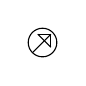
\begin{tikzpicture}
        \draw (0,0) circle (1.2ex);
        \draw (0.7 ex, 0.7 ex) -- (-0.4 ex, 0.7 ex);
        \draw (-0.4 ex, 0.7 ex) -- (0.7 ex, -0.4 ex);
        \draw (0.7 ex, -0.4 ex) -- (0.7 ex, 0.7 ex);
        \draw (0.7 ex, 0.7 ex) -- (-0.848 ex, -0.848 ex);
    \end{tikzpicture}}}
    \ \ 
}

% legendre符号
\makeatletter
\def\legendre@dash#1#2{\hb@xt@#1{%
  \kern-#2\p@
  \cleaders\hbox{\kern.5\p@
    \vrule\@height.2\p@\@depth.2\p@\@width\p@
    \kern.5\p@}\hfil
  \kern-#2\p@
  }}
\def\@legendre#1#2#3#4#5{\mathopen{}\left(
  \sbox\z@{$\genfrac{}{}{0pt}{#1}{#3#4}{#3#5}$}%
  \dimen@=\wd\z@
  \kern-\p@\vcenter{\box0}\kern-\dimen@\vcenter{\legendre@dash\dimen@{#2}}\kern-\p@
  \right)\mathclose{}}
\newcommand\legendre[2]{\mathchoice
  {\@legendre{0}{1}{}{#1}{#2}}
  {\@legendre{1}{.5}{\vphantom{1}}{#1}{#2}}
  {\@legendre{2}{0}{\vphantom{1}}{#1}{#2}}
  {\@legendre{3}{0}{\vphantom{1}}{#1}{#2}}
}
\def\dlegendre{\@legendre{0}{1}{}}
\def\tlegendre{\@legendre{1}{0.5}{\vphantom{1}}}
\makeatother
\addbibresource{Accessories/ref.bib}
\newcommand{\Yang}[1]{\textcolor{red}{#1}}


\title{Notes in Algebraic Geometry}
\author{Tianle Yang}
\date{\today}
\authoremail{\href{mailto:loveandjustice@88.com}{loveandjustice@88.com}}
\authorpage{\href{https://www.tianleyang.com}{tianleyang.com}}
\texsource{\href{https://github.com/MonkeyUnderMountain/Note_on_Algebraic_Geometry}{github.com/MonkeyUnderMountain/Note\_on\_Algebraic\_Geometry}}
\version{0.1.0}

\setCJKfamilyfont{lxgwwenkai}{LXGW WenKai} % 定义霞鹜文楷,若未安装,请去掉相关代码编译或使用其他字体
\coversentence{\CJKfamily{lxgwwenkai}「あんたバかァ?」}
\coverimage{Asuka.png} % 封面图片
\coverlinecolor{brown!80!yellow} % 封面横线颜色
\covertitlefont{Allura} % 封面标题字体, 若未安装,可注释掉此行编译或使用其他字体
\covertextcolor{red!80!black} % 封面标题颜色


\begin{document}

    % \pagestyle{empty}
    \maketitle

    \frontmatter

    \tableofcontents

    \mainmatter

    % \chapter{The First Properties}
    %     \section{Setup and the first examples}
\subsection{Notations}

    All schemes are assumed to be separated.
    For a ``scheme'' which is not separated, we will use the term ``prescheme''.

    Let $A$ be a ring.
    We denote by $\Spec A$ the spectrum of $A$.
    For an ideal $I \subset A$, we use $V(I)$ to denote the closed subscheme of $\Spec A$ defined by $I$.
 
    Let $S$ be $\Spec \kk$, $\Spec \calo_K$ or an algebraic variety.
    An $S$-variety is an integral scheme $X$ which is of finite type and flat over $S$.
    For an algebraic variety, we mean a $\kk$-variety.

    We will use $\kk,\KK$ to denote fields, and $\kkk,\KKK$ to denote their algebraically closure relatively.

    Let $X$ be an integral scheme.
    We denote by $\fkk(X)$ the function field of $X$.
    For a closed point $x \in X$, we denote by $\rkk(x)$ the residue field of $x$.

    We denote the category of $S$-varieties by $\Var_S$.
    We denote by $X(T)$ the set of $T$-points of $X$, that is, the set of morphisms $T \to X$.

    Let $X$ be an algebraic variety over $\kk$.
    A geometrical point is referred a morphism $\Spec \kkk \to X$.

    When refer a point (may not be closed) in a scheme, we will use the notation $\xi \in X$.
    We use $Z_\xi$ to denote the Zariski closure of $\{\xi\}$ in $X$.
    When we talk about a closed point on an algebraic variety, we will use the notation $x \in X(\kkk)$.

    \subsubsection{Separated and proper morphisms}


\subsection{Examples}

    % \begin{example}
    %     Let $\kkk$ be an algebraically closed field and $A$ the localization of $\kkk[x]$ at $(x)$.
    %     Let $S = \Spec A$ and $X = \Spec A[y]$. 
    %     There are three types of points in $X$:
    %     \begin{enumerate}[label=(\roman*)]
    %         \item closed points with residue field $\kkk$, like $p = (x,y-a)$;
    %         \item closed points with residue field $\kkk(y)$, like $P = (xy-1)$;
    %         \item non-closed points, like $\eta_1 = (x),\eta_2 = (y),\eta_3 = (x-y)$.
    %     \end{enumerate}

    % \end{example}

% \subsection{Preparation in commutative algebra}

%     \subsubsection{Nakayama's Lemma \Yang{To be completed}}

%         \begin{theorem}[Nakayama's Lemma]\label{thm: Nakayama's lemma}
%             Let $A$ be a ring and $\frakM$ be its Jacobi radical.
%             Suppose $M$ is a finitely generated $A$-module.
%             If $\fraka M = M$ for $\fraka \subset \frakM$, then $M = 0$.
%         \end{theorem}
%         \begin{proof}
%             Suppose $M$ is generated by $x_1,\cdots,x_n$.
%             Since $M = \fraka M$, formally we have $(x_1,\cdots,x_n)^T = \Phi (x_1,\cdots, x_n)^T$ for $\Phi \in M_n(\fraka)$.
%             Then $(\Phi - \id) (x_1,\cdots, x_n)^T = 0$. 
%             Note that $\det (\Phi - \id) = 1+a$ for $a \in \fraka \subset \frakM$.
%             Then $\Phi-\id$ is invertible and then $M=0$.
%         \end{proof}

%         \begin{proposition}[Geometric form of Nakayama's Lemma]\label{prop: geometric form of Nakayama's lemma}
%             Let $X = \Spec A$ be an affine scheme, $x\in X$ a closed point and $\calf$ a coherent sheaf on $X$.
%             If $a_1,\cdots,a_k \in \calf(X)$ generate $\calf|_x = \calf \ten \rkk(x)$, then there is an open subset $U \subset X$ such that $a_i|_U$ generate $\calf(U)$. 
%         \end{proposition}
%         \begin{proof}
%             \Yang{To be completed.}
%         \end{proof}

%         \begin{corollary}\label{cor: upper semicontinuity of dim F|_y}
            
%         \end{corollary}
%         \begin{proof}
%             \Yang{To be completed.}
%         \end{proof}



%     \subsubsection{Associated prime ideals}

%         This part refers to \cite[Chapter 3]{Mat70}.

%         \begin{definition}[Associated prime ideals]\label{def: associated prime ideals}
%             Let $A$ be a noetherian ring and $M$ an $A$-module.
%             The \textit{associated prime ideals} of $M$ are the prime ideals $\frakp$ of form $\Ann(x)$ for some $x \in M$.
%             The set of associated prime ideals of $M$ is denoted by $\Ass(M)$.
%         \end{definition}

%         \begin{example}
%             Let $A = \kkk[x,y]/(xy)$ and $M = A$.
%             First we see that $(x) = \Ann y, (y) = \Ann x \in \Ass M$.
%             Then we check other prime ideals.
%             For $(x,y)$, if $xf = yf = 0$, then $f \in (x) \cap (y) = (0)$.
%             If $(x-a) = \Ann f$ for some $f$, note that $y \in (x-a)$ for $a \in \kkk^*$, then $f \in (x)$.
%             Hence $f = 0$. 
%             Therefore $\Ass M = \{ (x), (y) \}$.
%         \end{example}

%         \begin{example}
%             Let $A = \kkk[x,y]/(x^2, xy)$ and $M = A$.
%             The underlying space of $\Spec A$ is the $y$-axis since $\sqrt{(x^2,xy)} = (x)$.
%             First note that $(x) = \Ann y, (x,y) = \Ann x \in \Ass M$.
%             For $(x,y-a)$ with $a \in \kkk^*$, easily see that $xf = (y-a)f = 0$ implies $f=0$ since $A = \kkk \cdot x \oplus \kkk[y]$ as $\kkk$-vector space.
%             Hence $\Ass M = \{ (x), (x,y) \}$.
%         \end{example}

%         Let $A$ be a noetherian ring and $M$ an $A$-module.
%         Note that $S^{-1}M = 0$ if and only if $S \cap \Ann M \neq \emptyset$.
%         Then the set 
%         \[ \{ \frakp \in \Spec A \colon M_\frakp \neq 0 \} \]
%         is equal to $V(\Ann M)$.
        
%         \begin{definition}\label{def: support of a module}
%             Let $A$ be a noetherian ring and $M$ an $A$-module.
%             The \textit{support} of $M$ is the closed subset $V(\Ann M)$ of $\Spec A$, denoted by $\Supp M$.
%         \end{definition}

%         \begin{lemma}\label{lem: maximal Ann(x) is prime}
%             Let $A$ be a noetherian ring and $M$ an $A$-module.
%             Then the maximal element of the set 
%             \[ \{ \Ann x \colon x \in M_\frakp, x \neq 0 \} \]
%             belongs to $\Ass M$.
%         \end{lemma}
%         \begin{proof}
%             We just need to show that such $\Ann x$ is prime.
%             Otherwise, there exist $a,b \in A$ such that $ab \in \Ann x$ but $a,b \notin \Ann x$.
%             It follows that $\Ann x \subsetneq \Ann ax$ since $b \in \Ann ax \setminus \Ann x$.
%             This contradicts the maximality of $\Ann x$.
%         \end{proof}

%         An element $a \in A$ is called a zero divisor for $M$ if $M \to aM, m\mapsto am$ is not injective.

%         \begin{corollary}\label{cor: zero divisors and associated prime ideals}
%             Let $A$ be a noetherian ring and $M$ an $A$-module.
%             Then 
%             \[ \{\text{zero divisors for } M \} = \bigcup_{\frakp \in \Ass M} \frakp. \]
%         \end{corollary}

%         \begin{lemma}\label{lem: associated set is stable under localization}
%             Let $A$ be a noetherian ring and $M$ an $A$-module.
%             Then $\frakp \in \Ass_A M$ iff $\frakp A_\frakp \in \Ass_{A_\frakp} M_\frakp$.
%         \end{lemma}
%         \begin{proof}
%             Suppose $\frakp A_\frakp\in \Ass_{A_\frakp} M_\frakp$.
%             Let $\frakp A_\frakp = \Ann y_0/c$ with $y_0 \in M$ and $c \in A \setminus \frakp$.
%             For $a \in \Ann y_0$, $ay_0 = 0$.
%             Then $a/1 \in \frakp A_\frakp$.
%             It follows that $a \in \frakp$.
%             Hence $\Ann y_0 \subset \frakp$.

%             Inductively, if $\Ann y_n \subsetneq \frakp$, then there exists $b_{n} \in A \setminus \frakp$ 
%             such that $y_{n+1}:=b_ny_n$, $\Ann y_{n+1} \subset \frakp$ and $\Ann y_n \subsetneq \Ann y_{n+1}$.
%             To see this, choose $a_n \in \frakp\setminus \Ann y_n$.
%             Then $(a_n/1) y_n = 0$ since $a_n/1 \in \frakp A_\frakp$.
%             By definition, there exist $b_n \in A \setminus \frakp$ such that $a_nb_ny_n = 0$.
%             This process must terminate since $A$ is noetherian.
%             Thus $\Ann y_n = \frakp$ for some $n$.
%             Hence $\frakp \in \Ass_A M$. 

%             Conversely, suppose $\frakp = \Ann x \in \Ass M$.
%             If $(a/s)(x/1) = 0 \in M_\frakp$, there exist $t \in A \setminus \frakp$ such that $tax = 0$.
%             It follows that $ta \in \frakp$ and then $(a/s) \in \frakp A_\frakp$.
%             Hence $\frakp A_\frakp \in \Ass_{A_\frakp} M_\frakp$.
%         \end{proof}

%         \begin{proposition}\label{prop: Ass is subset of Supp}
%             We have $\Ass M \subset \Supp M$.
%             Moreover, if $\frakp \in \Supp M$ satisfies $V(\frakp)$ is an irreducible component of $\Supp M$, then $\frakp \in \Ass M$.
%         \end{proposition}
%         \begin{proof}
%             For any $\frakp = \Ann x \in \Ass M$, we have $A/\frakp \cong A \cdot x \subset M$.
%             Tensoring with $A_\frakp$ gives $A_\frakp/\frakp A_\frakp \injmap M_\frakp$ since $A_\frakp$ is flat.
%             Hence $M_\frakp \neq 0$ and $\frakp \in \Supp M$.

%             Now suppose $\frakp \in \Supp M$ and $V(\frakp)$ is an irreducible component of $\Supp M$.
%             First we show that $\frakp \in \Ass_{A_\frakp} M_\frakp$.
%             Let $x \in M_\frakp$ such that $\Ann x$ is maximal in the set 
%             \[ \{ \Ann x \colon x \in M_\frakp, x \neq 0 \}. \]
%             Then we claim that $\Ann x = \frakp A_\frakp$.
%             First, $\Ann x$ is prime by Lemma \ref{lem: maximal Ann(x) is prime}.
%             If $\Ann x \neq \frakp$, then $V(\Ann x) \supset V(\frakp)$.
%             This implies that $\Ann x \notin \Supp M_\frakp$ since $\Supp M_\frakp = \Supp M \cap \Spec A_\frakp$.
%             This is a contradiction.
%             Thus $\frakp A_\frakp \in \Ass_{A_\frakp} M_\frakp$.
%             By Lemma \ref{lem: associated set is stable under localization}, we have $\frakp \in \Ass M$. 
%         \end{proof}

%         \begin{remark}
%             The existence of irreducible component is guaranteed by Zorn's Lemma.
%         \end{remark}

%         \begin{definition}\label{def: embedded prime}
%             A prime ideal $\frakp \in \Ass M$ is called \textit{embedded} if $V(\frakp)$ is not an irreducible component of $\Supp M$.
%         \end{definition}

%         \begin{example}
%             For $M = A = \kkk[x,y]/(x^2,xy)$, the origin $(x,y)$ is an embedded point.
%         \end{example}

%         \begin{proposition}\label{prop: Aass under exact sequence}
%             If we have exact sequence $0 \to M_1 \to M_2 \to M_3$, then $\Ass M_2 \subset \Ass M_1 \cup \Ass M_3$.
%         \end{proposition}
%         \begin{proof}
%             Let $\frakp = \Ann x \in \Ass M_2 \setminus \Ass M_1$.
%             Then the image $[x]$ of $x$ in $M_3$ is not equal to $0$.
%             We have that $\Ann x \subset \Ann [x]$.
%             If $a \in \Ann [x] \setminus \Ann x$, then $ax \in M_1$.
%             Since $\Ann x \subsetneq \Ann ax$, there is $b \in \Ann ax \setminus \Ann x$.
%             However, it implies $ba \in \Ann x$, and then $a \in \Ann x$ since $\Ann x$ is prime, which is a contradiction.
%         \end{proof}

%         \begin{corollary}\label{cor: Ass is finite}
%             If $M$ is finitely generated, then the set $\Ass M$ is finite.
%         \end{corollary}
%         \begin{proof}
%             For $\frakp = \Ann x \in \Ass M$, we know that the submodule $M_1$ generated by $x$ is isomorphic to $A/\frakp$.
%             Inductively, we can choose $M_n$ be the preimage of a submodule of $M/M_{n-1}$ which is isomorphic to $A/\frakq$ for some $\frakq \in \Ass M/M_{n-1}$.
%             We can take an ascending sequence $0 = M_0 \subset M_1 \subset \cdots \subset M_n \subset \cdots$ such that $M_i/M_{i-1} \cong A/\frakp_i$ for some prime $\frakp_i$.
%             Since $M$ is finitely generated, this is a finite sequence.
%             Then the conclusion follows by Proposition \ref{prop: Aass under exact sequence}.
%         \end{proof}

%         \begin{definition}\label{def: co-primary and primary}
%             An $A$-module is called \textit{co-primary} if $\Ass M$ has a single element.
%             Let $M$ be an $A$-module and $N \subset M$ a submodule.
%             Then $N$ is called \textit{primary} if $M/N$ is co-primary.
%             If $\Ass M/N = \{\frakp\}$, then $N$ is called $\frakp$-primary.
%         \end{definition}

%         \begin{remark}\label{rem: primary submodule and primary ideal}
%             This definition coincide with primary ideals in the case $M = A$.
%             Recall an ideal $\frakq \subset A$ is called \textit{primary} if $\forall ab \in \frakp$, 
%             $a \notin \frakq$ implies $b^n \in \frakq$ for some $n$. 
            
%             Let $\frakq$ be a $\frakq$-primary ideal.
%             Since $\Supp A/\frakq = \{\frakp\}$, $\frakp \in \Ass A/\frakq$.
%             Suppose $\Ann [a] \in \Ass A/\frakq$.
%             Then $\frakp \subset \Ann [a]$ since $V(\frakp) = \Supp A/\frakq$.
%             If $b \in \Ann [a]$, then $ab \in \frakq$ and $a\notin \frakq$.
%             Hence $b^n \in \frakq$, and then $b \in \frakp$.
%             This shows that $\Ass A/\frakq = \{\frakp\}$ and $\frakq$ is $\frakp$-primary as an $A$-submodule. 

%             Let $\frakq \subset A$ be a $\frakp$-primary $A$-submodule.
%             First we have $\frakp = \sqrt{\frakq}$ since $V(\frakp)$ is the unique irreducible component of $\Supp A/\frakq$.
%             Suppose $ab \in \frakq$ and $a\notin \frakq$.
%             Then $b \in \Ann [a] \subset \frakp$ since $\frakp$ is the unique maximal element in $\{ \Ann [c] \colon c \in A \setminus \frakq\}$.
%             This implies that $b^n \in \frakq$.
%         \end{remark}

%         \begin{definition}\label{def: minimal primary decomposition}
%             Let $A$ be a noetherian ring, $M$ an $A$-module and $N \subset M$ a submodule.
%             A \textit{minimal primary decomposition} of $N$ in $M$ is a finite set of primary submodules $\{Q_i\}_{i=1}^n$ such that 
%             \[ N = \bigcap_{i=1}^n Q_i, \] 
%             no $Q_i$ can be omitted and $\Ass M/Q_i$ are pairwise distinct.
%             For $\Ass M/Q_i = \{\frakp\}$, $Q_i$ is called belonging to $\frakp$.
%         \end{definition}

%         Indeed, if $N \subset M$ admits a minimal primary decomposition $N = \bigcap Q_i$ with $Q_i$ belonging to $\frakp$,
%         then $\Ass(M/N) = \{\frakp_i\}$.
%         For given $i$, consider $N_i := \bigcap_{j\neq i} Q_j$, then $N_i/N \cong (N_i+Q_i)/Q_i$.
%         Since $N_i \neq N$, $\Ass N_i/N \neq \emptyset$.
%         On the other hand, $\Ass N_i/N \subset \Ass M/Q_i = \{\frakp\}$.
%         It follows that $\Ass N_i/N = \{\frakp_i\}$, whence $\frakp_i \in \Ass M/N$.
%         Conversely, we have an injection $M/N \injmap \bigoplus M/Q_i$, so $\Ass M/N \subset \bigcup \Ass M/Q_i$.
%         Due to this, if $Q_i$ belongs to $\frakp$, we also say that $Q_i$ is the $\frakp$-component of $N$.
    
%         \begin{proposition}\label{prop: uniqueness of primary components}
%             Suppose $N\subset M$ has a minimal primary decomposition.
%             If $\frakp \in \Ass M/N$ is not embedded, then the $\frakp$ component of $N$ is unique.
%             Explicitly, we have $Q = \nu^{-1}(N_\frakp)$, where $\nu:M \to M_{\frakp}$.
%         \end{proposition}
%         \begin{proof}
%             First we show that $Q = \nu^{-1} (Q_\frakp)$.
%             Clearly $Q \subset \nu^{-1}(Q_\frakp)$.
%             Suppose $x \in \nu^{-1}(Q_\frakp)$.
%             Then there exists $s \in A \setminus \frakp$ such that $sx \in Q$.
%             That is, $[sx] = 0 \in M/Q$.
%             If $[x] \neq 0$, we have $s \in \Ann [x] \subset \frakp$.
%             This contradiction enforces $Q = \nu^{-1}(Q_\frakp)$.

%             Then we show that $N_\frakp = Q_\frakp$.
%             Just need to show that for $\frakp' \neq \frakp$ and the $\frakp'$ component $Q'$ of $N$, $Q'_\frakp = M_\frakp$.
%             Since $\frakp$ is not embedded, $\frakp' \not\subset \frakp$.
%             Then $\frakp \notin V(\frakp) = \Supp M/Q'$.
%             So $M_\frakp/Q'_\frakp = 0$.
%         \end{proof}

%         \begin{example}
%             If $\frakp$ is embedded, then its components may not be unique.
%             For example, let $M = A = \kkk[x,y]/(x^2,xy)$.
%             Then for every $n \in \bbz_{\geq 1}$, $(x) \cap (x^2,xy,y^n)$ is a minimal primary decomposition of $(0) \subset M$.
%         \end{example}

%         Let $A$ be a noetherian ring and $\frakp \subset A$ a prime ideal.
%         We consider the $\frakp$ component of $\frakp^n$, which is called $n$-th symbolic power of $\frakp$, denoted by $\frakp^{(n)}$.
%         We have $\frakp^{(n)} = \frakp^nA_\frakp \cap A$.
%         In general, $\frakp^{(n)}$ is not equal to $\frakp^n$; see below example.

%         \begin{example}
%             Let $A = \kk[x,y,z,w]/(y^2-zx^2,yz-xw)$ and $\frakp = (y,z,w)$.
%             We have $z = y^2/x^2,w = yz/x \in \frakp^2 A_\frakp$, whence $\frakp^2 A_\frakp = (z,w) \neq \frakp^2$.
%         \end{example}
        
%         \begin{theorem}\label{thm: primary decomposition for general module}
%             Let $A$ be a noetherian ring and $M$ an $A$-module.
%             Then for every $\frakp \in \Ass M$, there is a $\frakp$-primary submodule $Q(\frakp)$ such that 
%             \[ (0) = \bigcap_{\frakp \in \Ass M} Q(\frakp). \] 
%         \end{theorem}
%         \begin{proof}
%             Consider the set 
%             \[ \caln:= \{N \subset M \colon \frakp \notin \Ass N \}. \]
%             Note that $\Ass \bigcup N_i = \bigcup \Ass N_i$ by definition of associated prime ideals.
%             Then it is easy to check that $\caln$ satisfies the conditions of Zorn's Lemma.
%             Hence $\caln$ has a maximal element $Q(\frakp)$.
%             We claim that $Q(\frakp)$ is $\frakp$-primary.
%             If there is $\frakp' \neq \frakp \in \Ass M/Q(\frakp)$, then there is a submodule $N' \cong A/\frakp$.
%             Let $N''$ be the preimage of $N'$ in $M$.
%             We have $Q(\frakp) \subsetneq N''$ and $N'' \in \caln$.
%             This is a contradiction.
%             By the fact $\Ass \bigcap N_i = \bigcap \Ass N_i$, we get the conclusion.
%         \end{proof}

%         \begin{corollary}\label{cor: primary decomposition for finitely generated module}
%             Let $A$ be a noetherian ring and $M$ a finitely generated $A$-module.
%             Then every submodule of $M$ has a minimal primary decomposition.
%         \end{corollary}


%     \subsubsection{Length of modules}

%         \begin{definition}\label{def: length of a module}
%             Let $A$ be a ring and $M$ an $A$ module.
%             \textit{A simple module filtration of $M$} is a filtration
%             \[ M = M_0 \supsetneq M_1 \supsetneq \cdots \supsetneq M_n = 0 \] 
%             such that $M_i/M_{i-1}$ is a simple module, i.e. it has no submodule except $0$ and itself.
%             If $M$ has a simple module filtration as above, we define the \textit{length of $M$} as $n$ and say that $M$ has \textit{finite length}.
%         \end{definition}

%         The following proposition guarantees the length is well-defined.

%         \begin{proposition}\label{prop: length of a module is well defined}
%             Suppose $M$ has a simple module filtration $M = M_{0,0} \supsetneq M_{1,0} \supsetneq \cdots \supsetneq M_{n,0} = 0$.
%             Then for any other filtration $M = M_{0,0} \supset M_{0,1} \supset \cdots \supset M_{0,m} = 0$ with $m > n$, there exist $k<m$ such that $M_{0,k} = M_{0,k+1}$.
%         \end{proposition}
%         \begin{proof}
%             We claim that there are at least $0\leq k_1<\cdots<k_{m-n}<m$ satisfies that $M_{0,k_i} = M_{0,k_i+1}$.
%             Let $M_{i,j} := M_{i,0} \cap M_{0,j}$.
%             Inductively on $n$, we can assume that there exist $k_1,\cdots,k_{n-m+1}$ such that $M_{1,k} = M_{1,k+1}$.
%             Consider the sequence 
%             \[ M_{0,0}/M_{1,0} \supset (M_{0,1}+M_{1,0})/M_{1,0} \supset \cdots \supset (M_{0,m}+M_{1,0})/M_{1,0} = 0 \]
%             in $M_{0,0}/M_{1,0}$.
%             Since $M_{0,0}/M_{1,0}$ is simple, there is at most one $k_i$ with $M_{0,k_i}+M_{1,0} \neq M_{0,k_i+1}+M_{1,0}$.
%             And note that if $M_{0,k_i} + M_{1,0} = M_{0,k_i+1}+M_{1,0}$ and $M_{0,k_i} \cap M_{1,0} = M_{0,k_i} \cap M_{1,0}$, then $M_{0,k_i} = M_{0,k_i+1}$ by the Five Lemma.
%         \end{proof}

%         \begin{example}\label{eg: A/m is a simple module}
%             Let $A$ be a ring and $\frakm \in \mSpec A$.
%             Then $A/\frakm$ is a simple module.
%         \end{example}

%         \begin{proposition}\label{prop: of finite length iff both acc and dcc}
%             Let $A$ be a ring and $M$ an $A$-module.
%             Then $M$ is of finite length iff it satisfies both a.c.c and d.c.c.
%         \end{proposition}
%         \begin{proof}
%             Note that if $M$ has either a strictly ascending chain or a strictly descending chain, $M$ is of infinite length.
%             Conversely, d.c.c guarantee $M$ has a simple submodule and a.c.c guarantee the sequence terminates.
%         \end{proof}

%         \begin{proposition}\label{prop: length is additive for modules of finite length}
%             The length $l(-)$ is an additive function for modules of finite length.
%             That is, if we have an exact sequence $0 \to M_1 \to M_2 \to M_3 \to 0$ with $M_i$ of finite length, then $l(M_2) = l(M_1) + l(M_3)$.
%         \end{proposition}
%         \begin{proof}
%             The simple module filtrations of $M_1$ and $M_3$ will give a simple module filtration of $M_2$.
%         \end{proof}

%         \begin{proposition}\label{prop: characteristic of local artinian rings}
%             Let $(A,\frakm)$ be a local ring.
%             Then $A$ is artinian iff $\frakm^n = 0$ for some $n\geq 0$.    
%         \end{proposition}
%         \begin{proof}
%             Suppose $A$ is artinian.
%             Then the sequence $\frakm \supset \frakm^2 \supset \frakm^3 \supset \cdots$ will stable.
%             It follows that $\frakm^n = \frakm^{n+1}$ for some $n$.
%             By the Nakayama's Lemma \ref{thm: Nakayama's lemma}, $\frakm^n = 0$.

%             Conversely, we have 
%             \[ \frakm \subset \frakN \subset \bigcap_{\text{minimal prime ideal}} \frakp,\] 
%             whence $\frakm$ is minimal.
%         \end{proof}

%         \begin{proposition}\label{prop: artinian ring is of finite length}
%             Let $A$ be a ring. 
%             Then $A$ is artinian iff $A$ is of finite length.
%         \end{proposition}
%         \begin{proof}
%             First we show that $A$ has only finite maximal ideal.
%             Otherwise, consider the set $\{\frakm_1 \cap \frakm_2 \cap \cdots \cap \frakm_k\}$.
%             It has a minimal element $\frakm_1 \cap \cdots \cap \frakm_n$ and for any maximal ideal $\frakm$, $\frakm_1 \cap \cdots \cap \frakm_n \subset \frakm$.
%             It follows that $\frakm = \frakm_i$ for some $i$.
%             Let $\frakM = \frakm_1 \cap \cdots \cap \frakm_n$ be the Jacobi radical of $A$.
%             Consider the sequence $\frakM \supset \frakM^2 \supset \cdots$ and by Nakayama's Lemma, we have $\frakM^k = 0$ for some $k$.
%             Consider the filtration 
%             \[ A \supset \frakm_1 \supset \cdots \supset \frakm_1^k \supset \frakm_1^k\frakm_2 \supset \cdots \supset \frakm_1^k \cdots \frakm_n^k  = (0). \] 
%             We have $\frakm_1^k\cdots\frakm_i^j/\frakm_1^k\cdots\frakm_i^{j+1}$ is an $A/\frakm_i$-vector space.
%             It is artinian and then of finite length.
%             Hence $A$ is of finite length.
%         \end{proof}
        
%         \begin{proposition}\label{prop: artinian ring is of codimension 0}
%             Let $A$ be a ring. 
%             Then $A$ is artinian iff $A$ is noetherian and of dimension $0$.
%             For definition of dimension, see \ref{def: height of ideals}.
%         \end{proposition}
%         \begin{proof}
%             Suppose $A$ is artinian.
%             Then $A$ is noetherian by Proposition \ref{prop: artinian ring is of finite length}.
%             Let $\frakp \in \Spec A$.
%             Then $A/\frakp$ is an artinian integral domain.
%             If there is $a\in A/\frakp$ is not invertible, consider $(a) \supset (a^2) \supset \cdots$, we see $a=0$.
%             Hence $\frakp$ is maximal and $\dim A = 0$. 

%             Suppose that $A$ is noetherian and of dimension $0$.
%             Then every maximal ideal is minimal.
%             In particular, $A$ has only finite maximal ideal $\frakp_1,\cdots,\frakp_n$.
%             Let $\frakq_i$ be the $\frakp_i$-component of $(0)$.
%             Then we have $A \injmap \bigoplus_i A/\frakq_i$.
%             We just need to show that $A/\frakq_i$ is of finite length as $A$-module.
%             If $\frakq_i \subset \frakp_j$, take radical we get $\frakp_i \subset \frakq_j$ and hence $i=j$.
%             So $A/\frakq_i$ is a local ring with maximal ideal $\frakp_i A/\frakq_i$.
%             Then every element in $\frakp_i A/\frakq_i$ is nilpotent.
%             Since $\frakp_i$ is finitely generated, $(\frakp_i A/\frakq_i)^k = 0$ for some $k$.
%             Then $A/\frakq_i$ is artinian and then of finite length as $A/\frakq_i$-module.
%             Then the conclusion follows.
%         \end{proof}


%     \subsubsection{Noether's Normalization Lemma and Hilbert's Nullstellensatz \Yang{To be completed.}}

%         \begin{theorem}[Noether's Normalization Lemma]\label{thm: Noether's Normalization Lemma}
%             Let $A$ be a $\kk$-algebra of finite type.
%             Then there is an injection $\kk[T_1,\cdots,T_d] \injmap A$ such that $A$ is finite over $\kk[T_1,\cdots,T_d]$.
%         \end{theorem}

%         \begin{remark}
%             Here $A$ does not need to be integral. 
%             For example, 
%         \end{remark}

%         \begin{theorem}[Hilbert's Nullstellensatz]\label{thm: Nullstellensatz}
%             Let $A$ be a 
%         \end{theorem} 
    %     % \section{Normal, Cohen-Macaulay and regular schemes}

\subsection{Height, Depth and Dimension \Yang{To be completed}}

    \paragraph{Krull dimension and height of prime ideals}
    Algebraically, we have the following definitions.
    \begin{definition}\label{def: height of ideals}
        Let $A$ be a noetherian ring.
        The \textit{height of a prime ideal} $\frakp$ in $A$ is defined as the maximum length of chains of prime ideals contained in $\frakp$, that is, 
        \[ \idealht(\frakp) := \sup\{ n \mid \exists \text{ a chain of prime ideals } \frakp_0 \subsetneq \frakp_1 \subsetneq \cdots \subsetneq \frakp_n = \frakp\}. \] 
        The \textit{Krull dimension} of $A$ is defined as 
        \[ \dim A := \max_{\frakp \in \Spec A}\idealht(\frakp). \]
    \end{definition}

    Geometrically, we have the corresponding definition.
    \begin{definition}\label{def: dimension of schemes}
        Let $X$ be a noetherian scheme.
        The \textit{codimension of an irreducible subscheme} $Y$ in $X$ is defined as the length of the longest chain of irreducible closed subsets containing $Y$, that is, 
        \[ \codim_X(Y) := \sup\{ n \mid \exists \text{ a chain of irreducible closed subsets } Y = Y_0 \subsetneq Y_1 \subsetneq \cdots \subsetneq Y_n\}. \] 
        The \textit{dimension} of $X$ is defined as
        \[ \dim X := \max_{\xi \in X}\codim_X Z_\xi. \]
    \end{definition}

    For an affine scheme $X = \Spec A$, above two definitions coincide by the correspondence of prime ideals and irreducible closed subsets.

    \begin{proposition}\label{prop: dimension of localization, height and codimension}
        Let $A$ be a noetherian ring and $\frakp \in \Spec A$.
        Then 
        \[ \idealht(\frakp) = \codim_{\Spec A} V(\frakp) = \dim A_{\frakp}. \]
    \end{proposition}

    \begin{lemma}\label{lem: finite inclusion induces surjective morphism}
        Let $A \subset B$ be noetherian rings such that $B$ is finite over $A$.
        Then the induced morphism $\Spec B \to \Spec A$ is surjective.
    \end{lemma}
    \begin{proof}
        For $\frakp \in \Spec A$, let $S:= A-\frakp$ and denote $S^{-1}B$ by $B_\frakp$.
        Then we have $A_\frakp \injmap B_\frakp$ and $B_\frakp$ is finite over $A_\frakp$.
        Let $\frakP B_\frakp$ be a maximal ideal of $B_\frakp$.
        We claim that $\frakP B_\frakp \cap A_\frakp$ is maximal.
        Indeed, consider $A_\frakp/(\frakP \cap A_\frakp) \injmap B_\frakp/\frakP B_\frakp$, the latter is finite over the former.
        This enforces $A_\frakp/(\frakP B_\frakp \cap A_\frakp)$ be a field.
        Hence $\frakP B_\frakp \cap A_\frakp = \frakp A_\frakp$, and then $\frakP \cap A = \frakp$.
    \end{proof}

    \begin{proposition}\label{prop: finite morphisms preserve dimension}
        Let $A \subset B$ be noetherian rings such that $B$ is finite over $A$.
        Then $\dim A = \dim B$.
    \end{proposition}
    \begin{proof}
        If we have a sequence $\frakP_1 \subsetneq \frakP_2$ of prime ideals in $B$, then there exists $f \in \frakP_2 \setminus \frakP_1$.
        Since $B$ is finite over $A$, there exist $a_1,\cdots,a_n \in A$ such that 
        \[ f^n + a_1f^{n-1} + \cdots + a_n = 0.\]

        Then $a_n \in \frakP_2 \cap A$.
        If $a_n \in \frakP_1$, $f^{n-1} + \cdots + a_{n_1} \in \frakP_1$ since $f \notin \frakP_1$.
        Then $a_{n-1} \in \frakP_2$.
        Repeat the process, it will terminate, whence $\frakP_1 \cap A \subsetneq \frakP_2 \cap A$.
        Otherwise, we have $f^n \in a_1 B+ \cdots + a_nB \subset \frakP_1$.

        Conversely, suppose we have $\frakp_1,\frakp_2 \in \Spec A$ with $\frakp_1 \subsetneq \frakp_2$.
        Choose $\frakP_1 \in \Spec B$ such that $\frakP_1 \cap A = \frakp_1$, then we have $A/\frakp_1 \subset B/\frakP_1$.
        Let $\frakP_2$ be the preimage of the prime ideal in $B/\frakP_1$ which is over image of $\frakp_2$ in $A/\frakp_1$.
        Proposition \ref{lem: finite inclusion induces surjective morphism} guarantees that such $\frakP_2$ exists.
        Then we get $\frakP_1 \subsetneq \frakP_2$.
        Repeat this progress, we get $\dim B \geq \dim A$.
    \end{proof}

    \begin{theorem}[Krull's Principal Ideal Theorem]\label{thm: Krull's principal ideal theorem}
        Let $A$ be a noetherian ring.
        Suppose $f \in A$ is not a unit.
        Let $\frakp$ be a minimal prime ideal among those containing $f$.
        Then $\idealht(\frakp)\leq 1$.
        % Moreover, if $A$ is local or $\dim A_\frakm$ is constant for all $\frakm$, then the equality holds.
    \end{theorem}
    \begin{proof}
        By replacing $A$ by $A_\frakp$, we may assume $A$ is local with maximal ideal $\frakp$.
        Note that $A/(f)$ is artinian since it has only one prime ideal $\frakp/(f)$.

        Let $\frakq \subsetneq \frakp$.
        Consider the sequence $\frakq^{(1)} \supset \frakq^{(2)} \supset \cdots$, its image in $A/(f)$ is stationary.
        Then there exists $n \in \bbz_{\geq 0}$ such that $\frakq^{(n)} + (f) = \frakq^{(n+1)} +(f)$.
        For $x \in \frakq^{(n)}$, we may write $x = y + af$ for $y \in \frakq^{(n+1)}$.
        Then $af \in \frakq^{(n)}$.
        Since $\frakq^{(n)}$ is $\frakq$-primary and $f \notin \frakq$, $a \in \frakq^{(n)}$.
        Then we get $\frakq^{(n)} = \frakq^{(n+1)} + f \frakq^{(n)}$.
        That is, $\frakq^{(n)}/\frakq^{(n+1)} = f \frakq^{(n)}/\frakq^{(n+1)}$.
        Note that $f \in \frakp$, by Nakayama's Lemma, $\frakq^{(n)} = \frakq^{(n+1)}$.
        That is, $\frakq^n A_\frakq = \frakq^{n+1} A_\frakq$.
        By Nakayama's Lemma again, $\frakq^n A_\frakq = 0$.
        It follows that $\frakq A_\frakq$ is minimal, whence $A_\frakq$ is artinian.
        Therefore, $\frakq$ is minimal in $A$.
    \end{proof}

    \begin{corollary}\label{cor: geometric form of principal ideal theorem}
        Let $A$ be a noetherian local ring.
        Suppose $f \in A$ is not a unit.
        Then $\dim A/(f) \geq \dim A - 1$.
        If $f$ is not contained in a minimal prime ideal, the equality holds.
    \end{corollary}
    \begin{proof}
        Let $\frakp_0 \subsetneq \cdots \subsetneq \frakp_n$ be a sequence of prime ideals.
        By assumption, $f \in \frakp_n$.
        If $f \in \frakp_0$, we get a sequence of prime ideals in $A/(f)$ of length $n$.
        Now we suppose $f \notin \frakp_0$.
        Then there exists $k \geq 0$ such that $f \in \frakp_{k+1} \setminus \frakp_{k}$. 
            
        Choose $\frakq$ be a minimal prime ideal among those containing $(\frakp_{k-1},f)$ and contained in $\frakp_{k+1}$.
        Then by Krull's Principal Ideal Theorem \ref{thm: Krull's principal ideal theorem}, $\frakq_k \subsetneq \frakp_{k+1}$.
        Replace $\frakp_k$ by $\frakq_k$, we have $f \in \frakq_{k} \setminus \frakp_{k-1}$

        Repeat this process, we get a sequence $\frakp_0' \subsetneq \cdots \subsetneq \frakp_n'$ such that $f \in \frakp_1'$.
        This gives a sequence $\frakp_1' \subsetneq \cdots \subsetneq \frakp_n'$ in $A/(f)$.
        Hence we get $\dim A/(f) \geq \dim A - 1$.
 
        % Then there exist a prime ideal $\frakp_0 \subsetneq (f)$.
        Since $f$ is not contained in minimal prime ideal, preimage of a minimal prime ideal in $A/(f)$ has height $1$.
        Hence a sequence of prime ideals in $A/fA$ can be extended by a minimal prime ideal in $A$.
        It follows that $\dim A/(f) + 1 \leq \dim A$.
    \end{proof}

    For varieties, the Krull dimension behaves well by follows.

    \begin{lemma}\label{lem: dimension of algebraic varieties}
        Let $X$ be an algebraic variety over $\kk$.
        Then for every closed point $x \in X(\kkk)$, we have 
        \[ \dim X = \dim \calo_{X,x} = \trdeg(\fkk(X)/\kk). \] 
    \end{lemma}
    \begin{proof}
        Since $X$ is irreducible, we may assume that $X = \Spec A$ is affine.
        Let $d = \trdeg(\fkk(X)/\kk)$.

        By Noether's Normalization Lemma \ref{thm: Noether's Normalization Lemma}, there is an injective and finite homomorphism $A_0 = \kk[T_1,\cdots,T_d] \injmap A$.
        Let $\frakM$ be the corresponding maximal ideal of $x$ in $A$ and $\frakm = \frakM \cap \kk[T_1,\cdots,T_d]$.
        Denote the image of $T_i$ in $\exk:=A_0/\frakm$ by $t_i$.
        The extension $\exk/\kk$ is finite by Nullstellensatz \ref{thm: Nullstellensatz}.
        Let $f_i\in \kk[T]$ be the minimal polynomial of $t_i$ and $g_i:= f_i(T_i) \in A_0$.
        Then $g_i \in \frakm$ and $\frakm = g_1A_0 +\cdots,g_d A_0$.
        In particular, $g_1,\cdots,g_d \in \frakM$.

        We have $A/g_1A+\cdots+g_dA$ is finite over $A_0/\frakm$, whence it is artinian.
        This implies that $A_\frakM/g_1A_\frakM + \cdots + g_dA_\frakM$ is also artinian.
        Since $g_{k+1}$ is not a zero divisor in $A_0/g_1A_0+\cdots+g_kA_0$, $g_{k+1}$ is not contained in any minimal prime ideal of $A_0/g_1A_0+\cdots+g_kA_0$.
        Then $g_{k+1}$ is also not contained in any minimal prime ideal of $A/g_1A+\cdots+g_kA$.
        By Corollary \ref{cor: geometric form of principal ideal theorem}, $\dim A_\frakM = \dim (A_\frakM/g_1A_\frakM + \cdots + g_dA_\frakM) + d = d$.
    \end{proof}

    \begin{theorem}\label{thm: dimension of varieties}
        Let $S$ be spectrum of a field $\kk$ or an algebraic integer ring $\calo_K$ and $X$ an integral $S$-variety.
        Then we have the follows:
        \begin{enumerate}[label=(\roman*)]
            \item For every point $\xi \in X$, $\dim X = \dim \calo_{X,\xi} + \codim Z_\xi$.
            \item For every non-empty open subset $U \subset X$, $\dim U = \dim X$.
            \item $\dim X = \trdeg(\fkk(X)/\fkk(S)) + \dim S$.
        \end{enumerate}
    \end{theorem}
    \begin{proof}
        \Yang{To be continued.}
    \end{proof}

    \begin{example}
        For general noetherian schemes, Theorem \ref{thm: dimension of varieties} may not hold.
        Let $A = \kk[t]$, $\frakm = (t)$, $B=A_\frakm[x]$ and $X = \Spec B$.
        Then we have $\dim X = 2$ since 
        \Yang{To be added.}
    \end{example}


    \paragraph{Depth}
    For a noetherian local ring $(A,\frakm)$, we can define the depth of an $A$-module $M$.
    Somehow the Krull dimension is ``homological'' and the depth is ``cohomological''.

    \begin{definition}\label{def: regular sequence}
        Let $A$ be a noetherian ring, $I \subset A$ an ideal and $M$ a finitely generated $A$-module.
        A sequence $t_1,\cdots,t_n\in \frakm$ is called an \textit{$M$-regular sequence in $I$} if $t_i$ is not a zero divisor on $M/(t_1,\cdots,t_{i-1})M$ for all $i$. 
    \end{definition}

    \begin{example}
        Let $A = \kk[x,y]/(x^2,xy)$ and $I = (x,y)$.
        Then $\depth_I A = 0$.
    \end{example}

    % \begin{proposition}\label{lem: permutation of regular sequence is still regular}
    %     Suppose $A$ is local and $I = \frakm$ is the maximal ideal of $A$.
    %     Then any permutation of an $M$-regular sequence is $M$-regular.
    % \end{proposition}
    % \begin{proof}

    %     \Yang{To be completed.}
    % \end{proof}

    \begin{definition}
        The \textit{$I$-depth} of $M$ is defined as the maximum length of $M$-regular sequences in $I$, denoted by $\depth_I M$. 
        When $A$ is a local ring with maximal ideal $\frakm$, we write $\depth M$ for $\depth_{\frakm} M$.
    \end{definition}

    \paragraph{Regular and Serre's conditions}
    Up to now, there are three numbers measuring the ``size'' of a local ring $(A,\frakm)$:
    \begin{itemize}
        \item $\dim A$: the Krull dimension of $A$.
        \item $\depth A$: the depth of $A$.
        \item $\dim_{\rkk(\frakm)} T_{A,\frakm}$: the dimension of Zariski tangent space $T_{A,\frakm} := (\frakm/\frakm^2)^\lor$ as a ${\rkk(\frakm)}$-vector space.
    \end{itemize}

    These three numbers are related by the following inequalities.
    \begin{proposition}\label{prop: inequality of depth, dimension and dimension of tangent space}
        Let $(A,\frakm)$ be a local noetherian ring with residue field $\kk$.
        Then the following inequalities hold:
        \[ \depth A \leq \dim A \leq \dim_\kk T_{A,\frakm}. \]
    \end{proposition}
    \begin{proof}
        The first inequality is a direct corollary of Corollary \ref{cor: geometric form of principal ideal theorem}.

        Let $t_1,\cdots,t_n$ be a $\rkk(\frakm)$-basis of $\frakm/\frakm^2$.
        Then we have $\frakm/(t_1,\cdots,t_n)+\frakm^2 = 0$, whence $\frakm/(t_1,\cdots,t_n) = \frakm(\frakm/(t_1,\cdots,t_n))$.
        It follows that $\frakm = (t_1,\cdots,t_n)$ by Nakayama's Lemma.
        By Corollary \ref{cor: geometric form of principal ideal theorem}, 
        \[ n + \dim A/(t_1,\cdots,t_n) \geq n-1 + \dim A/(t_1,\cdots,t_{n-1}) \geq \cdots \geq 1 + \dim A/(t_1) \geq \dim A. \]  
        We conclude the result.
    \end{proof}

    % To see these, we need the following well-known theorem.

    \begin{definition}\label{def: regular and Serre's conditions}
        Let $X$ be a locally noetherian scheme and $k \in \bbz_{\geq 0}$.
        We say that \textit{$X$ verifies property $(R_k)$} or \textit{is regular in codimension $k$} if $\forall \xi \in X$ with $\codim Z_\xi \leq k$, 
        \[ \dim_{\rkk(\xi)} T_{X,\xi} = \dim \calo_{X,\xi}. \]
        We say that \textit{$X$ verifies property $(S_k)$} if $\forall \xi \in X$ with $\depth \calo_{X,\xi} < k$,
        \[ \depth \calo_{X,\xi} = \dim \calo_{X,\xi}. \]        
    \end{definition}

    \begin{lemma}\label{lem: trick lemma: subideal in union of prime belongs one}
        Let $A$ be a ring and $\fraka \subset \bigcup_i \frakp_i$.
        Then $\fraka \subset \frakp_i$ for some $i$.
    \end{lemma}
    \begin{proof}
        \Yang{To be completed.}
    \end{proof}

    \begin{example}\label{eg: S_1 is equivalent to A has no embedded point}
        Let $A$ be a noetherian ring.
        Then $A$ verifies $(S_1)$ iff $A$ has no embedded point.
        
        Suppose $A$ verifies $(S_1)$.
        If $\frakp \in Ass A$, every element in $\frakp$ is a zero divisor.
        Then $\depth A_{\frakp} = 0$.
        It follows that $\dim A_\frakp = 0$ and then $\frakp$ is minimal. 

        Suppose $A$ has no embedded point.
        Let $\frakp \in \Spec A$ with $\depth A_\frakp = 0$.
        This means every element in $\frakp A_\frakp$ is a zero divisor.
        Then 
        \[ \frakp \subset \{\text{zero divisors in } A\} = \bigcup_{\text{minimal prime ideals}} \frakq. \]
        By Lemma \ref{lem: trick lemma: subideal in union of prime belongs one}, $\frakp = \frakq$ for some minimal $\frakq$, whence $\dim A_\frakp = 0$. 
    \end{example}

    \begin{example}\label{eg: S_2 is equivalent to A/fA has no embedded point}
        Let $A$ be a noetherian ring verifies $(S_1)$.
        Then $A$ verifies $(S_2)$ iff for any nonzero divisor $f \in A$, $\Ass_A A/fA$ has no embedded point.

        Suppose $A$ verifies $(S_2)$.
        Let $f \in A$ be a nonzero divisor and $\frakp \in \Ass_A A/fA$.
        There exist $g \in A \setminus fA$ such that $\frakp = (f:g)$.
        For any $t_1,t_2 \in \frakp$, there exist $s_1,s_2$ with $s_i \notin (t_i)$ and $t_i g = f s_i$.
        Then $t_1t_2g = fs_1t_2 = fs_2t_1$.
        Since $f$ is not a zero divisor, $s_1t_2 = s_2t_1$.
        Then $t_2$ is a zero divisor in $A_\frakp/t_1 A_\frakp$ since $s_1 \notin (t_1)$.
        Since $f \in \frakp$, $\depth A_\frakp = 1$ and then $\idealht \frakp = 1$.
        This show that $\frakp$ is not embedded in $\Ass_A A/fA$.
        
        Conversely, suppose $\Ass_A A/fA$ has no embedded point.
        Let $\frakp \in \Spec A$ with $\depth A_{\frakp} = 1$.
        Then there exists $f \in A_{\frakp}$ which is not a zero divisor.
        We have $\depth A_{\frakp}/fA_\frakp = 0$ and $\Ass_A A/fA$ has no embedded point, whence $\frakp$ is minimal in $A/fA$.
        Then $\idealht \frakp = 1$ by Krull's Principal Ideal Theorem \ref{thm: Krull's principal ideal theorem} and the fact $f$ is not a zero divisor.
    \end{example}

    \begin{example}\label{eg: R-S criterion of reducedness}
        Let $X$ be a locally noetherian scheme.
        Then $X$ is reduced iff it verifies $(R_0)$ and $(S_1)$.

        The properties are local, whence we can assume $X=\Spec A$.
        Suppose $A$ is reduced.
        Let $\frakp_1,\cdots,\frakp_n$ be all minimal prime ideals of $A$.
        We have $\bigcap \frakp_i = \frakN = (0)$, where $\frakN$ is the nilradical of $A$.
        Hence $A$ has no embedded point.
        Since $A_\frakp$ is artinian, local and reduced, $A_\frakp$ is a field and hence regular.
        
        Conversely, let $\Ass A$ be equal to $\{\frakp_1,\cdots,\frakp_n\}$.
        Then every $\frakp_i$ is minimal by $(S_1)$.
        Let $f$ be in $\frakN$.
        Then the image of $f$ in $A_{\frakp_i}$ is $0$ since by $(R_0)$, $A_{\frakp_i}$ is a field.
        It follows that $f \in \frakq_i$, where $\frakq_i$ is the $\frakp_i$ component of $(0)$ in $A$.
        Hence $f \in \bigcap \frakq_i = (0)$.
        That is, $A$ is reduced.
    \end{example}




\subsection{Normal schemes \Yang{To be completed}}

    % Fix a noetherian local ring $(A,\frakm)$ with residue field $\kk$.

    \begin{definition}\label{def: normal domain}
        An integral domain $A$ is called \textit{normal} if it is integrally closed in its field of fractions $\Frac(A)$.
    \end{definition}

    \begin{lemma}\label{lem: integral closed under localization}
        Let $A \subset C$ be rings and $B$ the integral closure of $A$ in $C$, $S$ a multiplicatively closed subset of $A$.
        Then the integral closure of  $S^{-1}A$ in $S^{-1}C$ is $S^{-1}B$.
    \end{lemma}
    \begin{proof}
            For every $b \in B$ and $\forall s \in S$, there exists $a_i \in A$ s.t. 
            \[ 
                b^n + a_1 b^{n-1} + \cdots + a_n = 0.
            \] 
            Then 
            \[ 
                \left( \frac{b}{s} \right)^n + \frac{a_1}{s^1} \left( \frac{b}{s} \right)^{n-1} + \cdots + \frac{a_n}{s^n} = 0.
            \] 
            Hence $b/s$ is integral over $S^{-1}A$, $S^{-1}B$ is integral over $S^{-1}A$.

            If $c/s \in S^{-1}C$ is integral over $S^{-1}A$, then $\exists a_i \in S^{-1}A$ s.t.
            \[ 
                \left( \frac{c}{s} \right)^n + a_1 \left( \frac{c}{s} \right)^{n-1} + \cdots + a_n = 0.
            \]
            Then 
            \[ 
                c^n + a_1 s c^{n-1} + \cdots + a_n s^n = 0 \in S^{-1}C
            \] 
            Then $\exists t \in S$ s.t. 
            \[
                t (c^n + a_1 s c^{n-1} + \cdots + a_n s^n) = 0 \in C.
            \] 
            Then 
            \[ 
                (ct)^n + a_1 s t (ct)^{n-1} + \cdots + a_n s^n t^n  = t^n (c^n + a_1 s c^{n-1} + \cdots + a_n s^n) = 0.
            \] 
            Hence $ct$ is integral over $A$, then $ct \in B$.
            Then $c/s = (ct)/(st) \in S^{-1}B$.
            This completes the proof.
    \end{proof}

    \begin{proposition}\label{prop: normality is a local property}
        Normality is a local property. 
        That is, for an integral domain $A$, TFAE:
        \begin{enumerate}[label=(\roman*)]
            \item $A$ is normal.
            \item For any prime ideal $\frakp \in \Spec A$, the localization $A_\frakp$ is normal.
            \item For any maximal ideal $\frakm \in \mSpec A$, the localization $A_\frakm$ is normal.
        \end{enumerate}
    \end{proposition}
    \begin{proof}
        When $A$ is normal, $A_\frakp$ is normal by Lemma \ref{lem: integral closed under localization}.

        Assume that $A_\frakm$ is normal for every $\frakm \in \mSpec A$.
        If $A$ is not normal, let $\tilde{A}$ be the integral closure of $A$ in $\Frac A$, $\tilde{A}/A$ is a nonzero $A$-module.
        Suppose $\frakp \in \Supp \tilde{A}/A$ and $\frakp \subset \frakm$.
        We have $\tilde{A}_\frakm/A_\frakm = 0$ and $\tilde{A}_\frakp/A_\frakp = (\tilde{A}_\frakm/A_\frakm)_\frakp \neq 0$.
        This is a contradiction.
    \end{proof}

    % \begin{proposition}
    %     Let $A$ be a normal ring.
    %     Then $A[X]$ is also normal.
    % \end{proposition}

    \begin{definition}\label{def: normal of scheme and general ring}
        A scheme $X$ is called \textit{normal} if the local ring $\calo_{X,\xi}$ is normal for any point $\xi \in X$.
        A ring $A$ is called \textit{normal} if $\Spec A$ is normal.
    \end{definition}

    \begin{remark}\label{rmk: total ring of fractions and normality of general reduced ring}
        For a general ring $A$, let $S := A\setminus (\bigcup_{\frakp \in \Ass A} \frakp) = \bigcap_{\frakp \in \Ass A}A\setminus \frakp$.
        Then $S$ is a multiplicative set.
        The localization $S^{-1}A$ is called \textit{the total ring of fractions} of $A$.
        
        Suppose $A$ is reduced and $\Ass A = \{\frakp_1,\cdots,\frakp_n\}$.
        Denote its total ring of fractions by $Q$.
        Note that elements in $Q$ are either unit or zero divisor.
        Hence any maximal ideal $\frakm$ is contained in $\bigcup \frakp_iQ$, whence contained in some $\frakp_i Q$.
        Thus $\frakp_i Q$ are maximal ideals.
        And we have $\bigcap \frakp_i Q = 0$. 
        By the Chinese Remainder Theorem, we have $Q = \prod Q/{\frakp_i}Q = \prod A_{\frakp_i}$.
        
        Let $A$ be a reduced ring with total ring of fractions $Q$.
        Then $A$ is normal iff $A$ is integral closed in $Q$.
        If $A$ is normal, then for every $\frakp \in \Spec A$, $A_\frakp$ is integral.
        Then there is unique minimal prime ideal $\frakp_i \subset \frakp$.
        In particular, any two minimal prime ideal are relatively prime.
        By the Chinese Remainder Theorem, $A = \prod A/\frakp_i$.
        Just need to check $A/\frakp_i$ is integral closed in $A_{\frakp_i}$.
        This is clear by check pointwise.

        Conversely, suppose $A$ is integral closed in $Q$.
        Let $e_i$ be the unit element of $A_{\frakp_i}$.
        It belongs to $A$ since $e_i^2 - e_i = 0$.
        Since $1 = e_1 + \cdots + e_n$ and $e_ie_j = \delta_{ij}$, we have $A = \prod Ae_i$.
        Since $Ae_i$ is integral closed in $A_{\frakp_i}$, it is normal.
        Hence $A$ is normal.
    \end{remark}

    \begin{definition}
        Let $X$ be a scheme.
        The \textit{normalization} of $X$ is an $X$-scheme $X^\nu$ with the following universal property:
        for any normal $X$-scheme $Y$ with dominant structure morphism, its structure morphism $Y \to X$ factors through $X^\nu$.
    \end{definition}

    \begin{proposition}
        The normalization $X^\nu$ of $X$ exists.
        Moreover, if $X$ is reduced, $X^\nu \to X$ is birational.
    \end{proposition}
    \begin{proof}
        Suppose there is a dominant morphism $Y \to X$ with $Y$ normal.
        Since $Y$ is normal, it is reduced.
        Then it factors through $X_{red}$.
        Hence we can assume that $X$ is reduced by replacing $X$ by $X_{red}$.

        Suppose $X = \Spec A$ is affine.
        Let $A^\nu$ be the integral closure of $A$ in it total ring of fractions and $X^\nu := \Spec A^\nu$.
        It gives a homomorphism $A \to \calo_Y(Y)$.
        We claim that it is injective.
        Otherwise, it factors through $A \to A/I$ and then $Y \to \Spec A$ factors through $\Spec A/I \to \Spec A$.
        It contradicts that $Y \to X$ is dominant.
        Since $Y$ is normal, $\calo_Y(Y)$ is integral closed in its total ring of fraction.
        Then $\calo_Y(Y)$ contains $A^\nu$.
        This shows that $X^\nu$ is the normalization of $X$.

        In general case, take an affine cover $\{U_i\}$ of $X$ and clue these $U_i^\nu$ by universal property.
    \end{proof}

    % \begin{proposition}
    %     Let $S = \Spec \kk$ or $\Spec \calo_K$ and $X$ an $S$-variety.
    %     Then the normalization $X^\nu \to X$ is birational.
    %     In particular, $\{ \xi \in X \colon \calo_{X,\xi} \text{ is normal} \}$ is open in $X$.
    % \end{proposition}

    \begin{lemma}\label{lem: normal rings verify R_1 and S_2}
        Let $A$ be a normal ring.
        Then $A$ verifies $(R_1)$ and $(S_2)$.
    \end{lemma}
    \begin{proof}
        Since all properties are local, we can assume $A$ is integral and local.

        For $(S_2)$, by Example \ref{eg: S_2 is equivalent to A/fA has no embedded point}, we only need to show that $\Ass_A A/f$ has no embedded point.
        Let $\frakp = (f:g) = \in \Ass_A A/fA$ and $t:= f/g \in \Frac A$.
        After Replacing $A$ by $A_\frakp$, we can assume that $\frakp$ is maximal.
        By definition, $t^{-1}\frakp \subset A$.
        If $t^{-1}\frakp \subset \frakp$, suppose $\frakp$ is generated by $(x_1,\cdots,x_n)$ and $t^{-1}(x_1,\cdots,x_n)^T = \Phi(x_1,\cdots,x_n)^T$ for $\Phi \in M_n(A)$.
        There is a monic polynomial $\chi(T) \in A[T]$ vanishing $\Phi$.
        Then $\chi(t^{-1}) = 0$ and $t^{-1} \in A$.
        This is impossible by definition of $t$.
        Then $t^{-1}\frakp = A$, and $\frakp = (t)$ is principal. 
        By Krull's Principal Ideal Theorem \ref{thm: Krull's principal ideal theorem}, $\idealht(\frakp) = 1$.

        Now we show that $A$ verifies $(R_1)$.
        Suppose $(A, \frakm)$ is local of dimension $1$.
        Choosing $a \in \frakm$, $A/a$ is of dimension $0$.
        Then by \ref{prop: characteristic of local artinian rings}, $\frakm^n \subset aA$ for some $n\geq 1$.
        Suppose $\frakm^{n-1} \not\subset aA$.
        Choose $b \in \frakm^{n-1} \setminus aA$ and let $t = a/b$.
        By construction, $t^{-1} \notin A$ and $t^{-1}\frakm \subset A$.
        After similar argument, we see that $\frakm = tA$, whence $A$ is regular.
    \end{proof}

    \begin{lemma}\label{lem: normal and regular are equivalent for noetherian rings of dimension 1}
        Let $(A,\frakm)$ be a noetherian local ring of dimension $1$.
        Then $A$ is normal iff $A$ is regular.
    \end{lemma}
    \begin{proof}
        By lemma \ref{lem: normal rings verify R_1 and S_2}, we just need to show that regularity implies normality.

        Let $t \in \frakm\setminus \frakm^2$.
        Since $A$ is regular, $\frakm = (t)$.
        Let $I \subset \frakm$ be an ideal.
        If $I \subset \bigcap_{n} \frakm^n$, then for every $a \in I$, there exists $a_n$ such that $a = a_n t^n$.
        Then we get an ascending chain of ideals $(a_1) \subset (a_2) \subset \cdots$.
        Hence $a=0$ by Nakayama's Lemma.
        Suppose $I$ is not zero.
        Then there is some $n$ such that $I \subset \frakm^n$ and $I \not\subset \frakm^{n+1}$.
        For every $at^n \in I \setminus \frakm^{n+1}$,  $a \notin \frakm$, whence $a$ is a unit in $A$.
        Then $I = (t^n)$.
        Hence $A$ is PID and hence normal.
    \end{proof}

    \begin{proposition}\label{prop: S_2 implies intersection of localization at height 1 prime is A}
        Let $A$ be a noetherian integral domain of dimension $\geq 1$ verifying $(S_2)$.
        Then 
        \[ A = \bigcap_{\frakp \in \Spec A, \idealht(\frakp) = 1} A_\frakp. \]
    \end{proposition}
    \begin{proof}
        Clearly $A \subset \bigcap A_\frakp$.
        Let $t = f/g \in \bigcap A_\frakp$.
        Since $f\in gA_\frakp$ and we have $g A = \bigcap (gA_\frakp \cap A)$, $f \in gA$.
        It follows that $t \in A$.
    \end{proof}

    \begin{theorem}[Serre's criterion for normality]
        Let $X$ be a locally noetherian scheme.
        Then $X$ is normal if and only if it verifies $(R_1)$ and $(S_2)$.
    \end{theorem}
    \begin{proof}
        One direction has been proved in Lemma \ref{lem: normal rings verify R_1 and S_2}.
        Suppose $X$ verifies $(R_1)$ and $(S_2)$.
        Again we can assume $X = \Spec A$ is affine and $A$ is local.
        By Remark \ref{rmk: total ring of fractions and normality of general reduced ring}, we just need to show that $A$ is integral closed in its total ring of fractions $Q$.
        Suppose we have 
        \[ \left(\frac{a}{b}\right)^n + c_1 \left(\frac{a}{b}\right)^{n-1} + \cdots + c_n = 0 \in Q. \]
        Since $A$ verifies $(S_2)$, $b A = \bigcap \nu_\frakp^{-1}(b_\frakp A_\frakp)$.
        So it is sufficient to show that $a_{\frakp} \in b_\frakp A_\frakp$ with $\idealht(\frakp) = 1$.
        Note that $A_\frakp$ is regular and hence normal by Lemma \ref{lem: normal and regular are equivalent for noetherian rings of dimension 1}.
        Then above equation gives us desired result.
    \end{proof}

    \begin{theorem}\label{thm: extension of function on normal scheme}
        Let $X$ be a normal and locally noetherian scheme.
        Let $F \subset X$ be a closed subset of codimension $\geq 2$.
        Then the restriction $H^0(X,\calo_X) \to H^0(X\setminus F, \calo_{X})$ is an isomorphism.
    \end{theorem}
    \begin{proof}
        By the exact sequences 
        \[ 0 \to \calf(X) \to \prod_i \calf(U_i) \to \prod_{i,j} \calf(U_i \cap U_j), \]
        where $\{U_i\}$ is an affine open cover of $X$, we can reduce to the case that $X$ is affine.
        Then $X = \Spec A$ for some normal noetherian ring $A$.
        For any prime ideal $\frakp \in \Spec A$ with $\idealht(\frakp) = 1$, we have $\frakp \in X \setminus F$.
        By Proposition \ref{prop: S_2 implies intersection of localization at height 1 prime is A}, the conclusion follows.
    \end{proof}

    \begin{theorem}[Valuation criterion for properness]\label{thm: valuation criterion for properness}
        Let $f:X \to Y$ be a morphism of finite type between noetherian schemes.
        Then $f$ is proper iff for any valuation ring $A$, $\KK = \Frac A$ and commutative diagram
        \[ \xymatrix{
            \Spec \KK \ar[r] \ar[d] & X \ar[d]^f \\
            \Spec A \ar[r] & Y
        }, \]
        the morphism $\Spec A \to Y$ factors through $f$ uniquely.
    \end{theorem}

    \begin{proposition}\label{prop: morphism defined on a generic point extends to a open subset}
        Let $X,Y$ be $S$-schemes with $S$ locally noetherian.
        Suppose $Y$ is of finite type over $S$.
        Let $\xi \in X$ and $f_x: \Spec \calo_{X,\xi} \to Y$ be a morphism.
        Then there exists an open subset $U \subset X$ containing $\xi$ such that the morphism extends to a morphism $U \to Y$.
    \end{proposition}
    \begin{proof}
        Replacing $S,X,Y$ by affine open neighborhoods of images of $\xi$, we can assume that $S = \Spec A$, $X=\Spec B$ and $Y = \Spec A[T_1,\cdots,T_n]/I$ are affine.
        Then we get a homomorphism $A[T_1,\cdots,T_n]/I \to B_{\xi}$ of $A$-algebra.
        Denote the image of $T_i$ by $f_i/g_i$ in $B_{\xi}$, where $f_i,g_i \in B$.
        Then above homomorphism factors through $B[1/g_1,\cdots,1/g_n] \to B_{\xi}$.
        Let $U$ be the open subset of $X$ defined by $g_1\cdots g_n \neq 0$.
        Then the morphism $f_x$ extends to a morphism $U \to Y$.
    \end{proof}

    \begin{theorem}\label{thm: extension of morphism form normal to proper}
        Let $X,Y$ be $S$-schemes of finite type with $S$ noetherian.
        Suppose $X$ is normal, and $Y$ is proper over $S$.
        Let $f:X \ratmap Y$ be a rational map.
        Then $f$ is well-defined on an open subset $U \subset X$ whose complement has codimension $\geq 2$.
    \end{theorem}
    \begin{proof}
        We can assume that $X$ is irreducible and hence integral.
        Suppose $f$ is defined on $U \subset X$.
        For every $\xi \in X$ with codimension $1$, we have following commutative diagram
        \[ \xymatrix{
            \Spec \fkk(X) \ar[r] \ar[d] & U \ar[r]^f & Y \ar[d] \\
            \Spec \calo_{X,\xi} \ar[rr] & & S
        }, \]
        By Theorem \ref{thm: valuation criterion for properness} and Proposition \ref{prop: morphism defined on a generic point extends to a open subset}, there exists an open subset $U_\xi \subset X$ containing $\xi$ such that the morphism extends to a morphism $U_\xi \to Y$.

        \Yang{To be completed.}
    \end{proof}

    \begin{remark}\label{rmk: extension of function on normal scheme and extension of morphism form normal to proper}
        Theorem \ref{thm: extension of function on normal scheme} and Theorem \ref{thm: extension of morphism form normal to proper} are very similar.
        However, they are base on different properties.
        Theorem \ref{thm: extension of function on normal scheme} is based on $(S_2)$, while Theorem \ref{thm: extension of morphism form normal to proper} is based on $(R_1)$.
        Philosophically, the $(S_k)$ conditions are used to control the ``bad part of codimension larger than $k$''.
        The $(R_k)$ conditions are used to control the ``bad part of codimension smaller than or equal to $k$''.
        We will see more examples in the next section.\Yang{To be completed.}
    \end{remark}




\subsection{Cohen-Macaulay schemes}

    \begin{definition}[Cohen-Macaulay]\label{def: Cohen-Macaulay}
        A noetherian local ring $(A,\frakm)$ is called \textit{Cohen-Macaulay} if $\dim A = \depth A$.
        A locally noetherian scheme $X$ is called \textit{Cohen-Macaulay} if $\calo_{X,\xi}$ is Cohen-Macaulay for any point $\xi \in X$.
    \end{definition}

    By definition, it is easy to see that $X$ is Cohen-Macaulay if and only if it verifies $(S_k)$ for all $k \geq 0$.

    \begin{example}[Non Cohen-Macaulay rings]

    \end{example}

    \begin{proposition}\label{prop: depth equals to grade}
        Let $(A, \frakm, \kk)$ be a noetherian local ring and $M$ a finite $A$-module.
        Then 
        \[ \depth M := \inf \{ i : \Ext^i_A(\kk,M) \neq 0 \}. \]
    \end{proposition}
    \begin{proof}
        Let $a \in \frakm$ be $M$-regular and $N = M/aM$.
        Then we claim that
        \[ \inf \{ i: \Ext^i_A(\kk,N) \neq 0 \} = \inf \{ i : \Ext^i_A(\kk,M) \neq 0 \} - 1. \]
        Indeed, we have an exact sequence
        \[ 0 \to M \xrightarrow{a} M \to N \to 0. \]
        It induces a long exact sequence
        \[ \cdots \to \Ext^{i-1}_A(\kk,M) \to \Ext^{i-1}_A(\kk,N) \to \Ext^i_A(\kk,M) \xrightarrow{\Ext^i_A(\kk,\Mult_a)} \Ext^i_A(\kk,M) \to \cdots. \]
        Note that $a \in \frakm$, then $\Ext^i_A(\kk,\Mult_a) = 0$.
        It follows that when $\Ext^{i-1}_A(\kk,M) = 0$, we have $\Ext^{i-1}_A(\kk,N) = 0$ iff $\Ext^i_A(\kk,M) = 0$, whence the claim.

        Let $n = \inf \{ i : \Ext^i_A(\kk,M) \neq 0 \}$.
        Induct on $n$.
        Suppose first $n = 0$.
        Since $\kk$ is a simple $A$-module, there is an injective homomorphism $\kk \to M$.
        Then $\frakm \in \Ass M$ and hence $\depth M = 0$.
        
        Suppose $n > 0$., let $a_1,\cdots,a_m \in \frakm$ be any $M$-regular sequence.
        Using the claim inductively on $M/(a_1,\cdots,a_m)M$, we have $n \geq \depth$.
        If $M$ has no regular element, then $\frakm \subset \bigcup_{\frakp \in \Ass M} \frakp$.
        Then $\frakm = \frakp$ for some $\frakp \in \Ass M$.
        This show that we can find $x \neq 0 \in M$ such that $\frakp = \Ann x$.
        It gives a homomorphism $\kk = A/\frakm \to M$.
        That is a contradiction and hence $M$ has a regular element.
        Let $a$ be $M$-regular and $N = M/aM$.
        Then $\depth N = n-1$ by the claim and induction hypothesis.
        Hence we have $\depth M \geq n$.
    \end{proof}

    \begin{corollary}\label{cor: induction on depth}
        Let $A$ be a noetherian ring, $M$ a finite $A$-module and $a \in A$ an $M$-regular element.
        Then $\depth M = \depth M/aM + 1$.
    \end{corollary}

    \begin{corollary}\label{cor: induction on S_d conditions}
        Let $A$ be a noetherian ring $a \in A$ a nonzero divisor.
        Then $A$ verifies $(S_d)$ iff $A/aA$ verifies $(S_{d-1})$.
    \end{corollary}

    \begin{definition}\label{def: unmixedness theorem}
        An ideal $I$ of a noetherian ring $A$ is called \textit{unmixed} if 
        \[ \idealht(I) = \idealht(\frakp), \quad \forall \frakp \in \Ass(A/I). \]
        Here $\idealht(I)$ is defined as 
        \[ \idealht(I) := \inf \{ \idealht(\frakp) : I \subset \frakp \}. \]
        We say that \textit{the unmixedness theorem holds for a noetherian ring $A$} if any ideal $I \subset A$ generated by $\idealht(I)$ elements is unmixed.
        We say that \textit{the unmixedness theorem holds for a locally noetherian scheme $X$} if $\calo_{X,\xi}$ is unmixed for any point $\xi \in X$.
    \end{definition}


    \begin{theorem}\label{thm: unmixedness theorem for Cohen-Macaulay schemes}
        Let $X$ be a locally noetherian scheme.
        Then the unmixedness theorem holds for $X$ if and only if $X$ is Cohen-Macaulay.
    \end{theorem}
    \begin{proof}
        We can assume that $X = \Spec A$ is affine.

        Suppose $X$ is Cohen-Macaulay.
        Let $I \subset A$ be an ideal generated by $a_1,\cdots,a_r$ with $r = \idealht(I)$.
        We claim that $a_1,\cdots,a_r$ is an $A$-regular sequence.
        If so, we get that the unmixedness theorem holds for $A$ by applying Example \ref{eg: S_1 is equivalent to A has no embedded point} on $A/I$. 
        Since $\idealht(a_1,\cdots,a_{r-1}) \leq r-1$ by Krull's Principal Ideal Theorem \ref{thm: Krull's principal ideal theorem} and $\idealht(a_1,\cdots,a_r) = r \leq \idealht(a_1,\cdots,a_{r-1}) + 1$, we have $\idealht(a_1,\cdots,a_{r-1}) = r-1$.
        By induction on $r$, we can assume that $a_1,\cdots,a_{r-1}$ is an $A$-regular sequence.
        Hence any prime ideal $\frakp \in \Ass A/(a_1,\cdots,a_{r-1})$ has height $r-1$.
        Now suppose $a_r$ is a zero divisor in $A/(a_1,\cdots,a_{r-1})$.
        Then there exists a prime ideal $\frakp \in \Ass A/(a_1,\cdots,a_{r-1})$ such that $a_r \in \frakp$.
        Then $I \subset \frakp$ and $\idealht(I) \leq r-1$.
        This contradicts that $\idealht(I) = r$.
        
        Suppose the unmixedness theorem holds for $A$.
        Let $\frakp \in \Spec A$ be a prime ideal with $\idealht(\frakp) = r$.
        Then $\frakp \in \Ass A$ if and only if $\idealht(\frakp) = 0$.
        If $r > 0$, there is a nonzero divisor $a \in \frakp$.
        By Krull's Principal Ideal Theorem \ref{thm: Krull's principal ideal theorem}, $\idealht(\frakp A/aA) = r-1$.
        Inductively, we can find a regular sequence $a_1,\cdots,a_r$ in $\frakp$.
        Then $\depth A_\frakp = r$.
        % \Yang{To be completed.}
    \end{proof}

    \begin{theorem}\label{thm: higher dimensional hartogs lemma for Cohen-Macaulay schemes}
        Let $X$ be a locally noetherian scheme.
        Suppose that $X$ is Cohen-Macaulay.
        Let $F \subset X$ be a closed subset of codimension $\geq k$.
        Then the restriction $H^i(X,\calo_X) \to H^i(X\setminus F, \calo_{X})$ induced by the 
         is an isomorphism.
    \end{theorem}
    \begin{proof}
        \Yang{To be completed.}
    \end{proof}


    
\subsection{Regular schemes}

    % \begin{proposition}
    %     Let $(A,\frakm)$ be a regular local ring.
    %     Then $A$ is integral.
    % \end{proposition}

    \begin{proposition}
        If $X$ verifies $(R_k)$, then $\codim_X X_{\text{sing}} \geq k+1$.
    \end{proposition}

    \begin{proposition}
        A regular scheme is Cohen-Macaulay.
    \end{proposition}

    \begin{corollary}
        A regular scheme is normal.
    \end{corollary}





    \chapter{Birational Geometry}
        \section{Bend and Break}

\subsection{Preliminary}

    \begin{definition}[Frobinius morphism]\label{def:Frobinius_morphism}
        Let \(X\) be a variety over a field \(\kkk\) of characteristic \(p > 0\).
        Denote the structure morphism by \(\pi: X \to \Spec \kkk\).
        The \emph{absolute Frobenius morphism} is the morphism given by \(\calo_X \to \calo_X, f \mapsto f^p\), denoted by \(\Frob_{X/\bbf_p}\).
        The \emph{relative Frobenius morphism} is the morphism \(\Frob_{X/\kkk}\) given by the following commutative diagram:
        \[ \xymatrix{
            X \ar@/^/[rrd]^{\Frob_{X/\bbf_p}}  \ar@/_/[ddr]_\pi \ar[rd]|{\Frob_{X/\kkk}}  &   & \\
                & X\times_{\kkk} \Spec \kkk \ar[r] \ar[d] & X \ar[d]^\pi \\
                & \Spec \kkk \ar[r]^{\Frob_{\kkk/\bbf_p}} &  \Spec \kkk
        }. \] 
        We usually denote \(X \times_{\kkk} \Spec \kkk\) appearing above by \(X^{(p)}\).
    \end{definition}

    \begin{proposition}\label{prop:relative_frobinius_is_finite_of_degree_p^d}
        Let \(X\) be a variety of dimension \(d\) over a field \(\kkk\) of characteristic \(p > 0\).
        Then the relative Frobenius morphism \(\Frob_{X/\kkk}: X \to X^{(p)}\) is a finite morphism of degree \(p^d\) over \(\kkk\).
    \end{proposition}

\subsection{Deformation of curves}

    \begin{theorem}[{ref. \cite[Chapter II, Theorem 1.2]{Kol96}}]\label{thm:dimension_of_deformation_space_of_curves}
        Let \(C\) be a smooth projective curve of genus \(g\) and \(X\) a smooth projective variety of dimension \(n\).
        Let \(f:C \to X\) be a non-constant morphism.
        Then every irreducible component of \(\Mor(C, X)\) containing \(f\) has dimension at least
        \[ -K_Y\cdot f(C) + (1-g)n. \]
    \end{theorem}

    \begin{proposition}\label{prop:deformation_of_curves_to_rational}
        Let \(X\) be a projective variety and \(f:C\to X\) a non-constant morphism from a pointed smooth projective curve \(p_0 \in C\).
        Let \(0 \in T\) be a pointed smooth curve (may not be projective).
        Suppose that we have a non-trivial family of morphisms \(f_t: C \to X\) for \(t \in T\) such that \(f_0 = f\) and \(f_t(p_0) = x_0\) for some point \(x_0 \in X\) and all \(t\).
        Then there exist some rational curves \(\Gamma_1, \ldots, \Gamma_m \subset X\) such that 
        \begin{enumerate}
            \item \(x_0 \in \bigcup_{i=1}^m \Gamma_i\);
            \item there is a morphism \(g: C \to X\) such that \(f(C) \equiv_{alg} g(C) + \sum_{i=1}^m a_i\Gamma_i\) with \(a_i > 0\) for all \(i\).
        \end{enumerate}
    \end{proposition}

    \begin{proposition}\label{prop:deformation_of_rational_curves_to_lower_degree}
        Let \(X\) be a projective variety and \(f:\bbp^1 \to X\) a non-constant morphism with \(f(0) = x_0, f(\infty) = x_\infty\).
        Let \(0 \in T\) be a pointed smooth curve (may not be projective).
        Suppose that we have a non-trivial family of morphisms \(f_t: \bbp^1 \to X\) for \(t \in T\) such that \(f_0 = f\) and \(f_t(0) = x_0, f_t(\infty) = x_\infty\) for all \(t\).
        Then there exists a curve \(C \subset X\) such that \(f(\bbp^1) \equiv_{alg} a C\) with \(a>1\).
    \end{proposition}

\subsection{Find rational curves}

    \begin{theorem}\label{thm:rational_curve_on_smooth_fano}
        Let \(X\) be a smooth Fano variety.
        Then for any \(x \in X(\kkk)\), there is a rational curve \(C\) passing through \(x\) with 
        \[ 0 < - C \cdot K_X \leq \dim X + 1. \]
    \end{theorem}
    \begin{proof}
        \Yang{To be completed.}
    \end{proof}

    \begin{theorem}\label{thm:rational_curve_on_smooth_variety_with_not_nef_K}
        Let \(X\) be a smooth projective variety such that \(K_X \cdot C < 0\) for some irreducible curve \(C \subset X\).
        Let \(H\) be an ample divisor on \(X\).
        Then there exists a rational curve \(\Gamma\) such that
        \[ -(K_X \cdot C) \cdot \frac{H\cdot \Gamma}{H \cdot C} \leq -K_X \cdot \Gamma \leq \dim X + 1. \]
    \end{theorem}
    \begin{proof}
        \Yang{To be completed.}
    \end{proof}

    \begin{theorem}\label{thm:rational_curve_on_exceptional_locus}
        Let \((X,B)\) be a projective klt pair and \(f:X \to Y\) a birational projective morphism.
        Suppose that \(K_{(X,B)}\) is \(f\)-ample.
        Then the exceptional locus of \(f\) is covered by rational curves \(\Gamma\) with 
        \[ 0 < -K_{(X,B)} \cdot \Gamma \leq 2\dim X. \]
    \end{theorem}

    \begin{theorem}\label{thm:general_rational_curve_on_smooth_variety_with_negative_intersection}
        Let \(X\) be a smooth projective variety of dimension \(n\) and \(H, H_1,\cdots,H_{n-1}\) ample divisors on \(X\).
        Suppose that \(K_X\cdot H_1 \cdots H_{n-1} < 0\).
        Then for a general point \(x\in X\), there exists a rational curve \(\Gamma\) passing through \(x\) such that
        \[ 0 < H \cdot \Gamma \leq - 2n \cdot \frac{H\cdot H_1 \cdots H_{n-1}}{K_X \cdot H_1 \cdots H_{n-1}}. \]
    \end{theorem}

    % \begin{proposition}\label{prop:general_rational_curve_on_klt_variety_with_negative_intersection}
    %     Let \(X\) be a normal projective variety of dimension \(n\) and \(H\) an ample divisor on \(X\).
    %     Suppose that \(K_X\cdot H^{n-1} < 0\).
    %     Then for a general point \(x\in X\), there exists a rational curve \(\Gamma\) passing through \(x\) such that
    %     \[ 0 < H \cdot \Gamma \leq - 2n \cdot \frac{H^n}{K_X \cdot H^{n-1}}. \]
    % \end{proposition}
        \section{Kodaira Vanishing Theorem}

\subsection{Preliminary}

    % \begin{theorem}[GAGA]\label{thm: GAGA for cohomology}
    %     Let $X$ be a smooth projective variety over $\mathbb{C}$ and \(\calF\) a coherent sheaf on \(X\).
    %     Then 
    %     \[
    %         H^i(X, \calF) \cong H^i(X^{an}, \calF^{an}).
    %     \]
    % \end{theorem}

    \begin{theorem}[Serre Duality]\label{thm: Serre duality for line bundles}
        Let \(X\) be a Cohen-Macaulay projective variety of dimension \(n\) over \(\kk\) and \(D\) a divisor on \(X\).
        Then there is an isomorphism
        \[
            H^i(X, D) \cong H^{n-i}(X, K_X - D)^\vee, \quad \forall i = 0, 1, \ldots, n.
        \]
    \end{theorem}

    % \begin{theorem}[Serre Vanishing]\label{thm: Serre vanishing theorem}
    %     Let \(X\) be a proper variety of dimension \(n\) over \(\kk\), \(\calF\) a coherent sheaf and \(\calL\) an ample line bundle on \(X\). 
    %     Then there exists an integer \(m_0 > 0\) such that for all \(m \geq m_0\),
    %     \[
    %         H^i(X, L^m\ten \calF) = 0,\quad \forall i > 0.
    %     \]
    % \end{theorem}

    \begin{theorem}[Log Resolution of Singularities]\label{thm: log resolution of singularities}
        Let X be an irreducible reduced algebraic variety over $\bbC$ (or a suitably small neighborhood of a compact set of an irreducible reduced analytic space) and $I \subset \calO_X$ a coherent sheaf of ideals defining a closed subscheme (or subspace) $Z$. Then there is a smooth variety (or analytic space) $Y$ and a projective morphism $f: Y \to X$ such that
        \begin{enumerate}
            \item $f$ is an isomorphism over $X - (\Sing(X) \cup \Supp Z)$,
            \item $f^*I \subset \calO_Y$ is an invertible sheaf $\calO_Y(-D)$ and 
            \item $\Exc(f) \cup D$ is an snc divisor.
        \end{enumerate}
    \end{theorem}

    \begin{theorem}[Lefschetz Hyperplane Theorem]\label{thm: Lefschetz hyperplane theorem}
        Let \(X\) be a smooth projective variety of dimension \(n\) over \(\bbC\) and \(Y\) a hyperplane section of \(X\).
        Then the restriction map
        \[
            H^k(X,\bbC) \to H^k(Y, \bbC)
        \]
        is an isomorphism for \(k < n - 1\) and an injection for \(k = n - 1\).
    \end{theorem}

    \begin{theorem}[Hodge Decomposition]\label{thm: Hodge decomposition}
        Let \(X\) be a smooth projective variety of dimension \(n\) over \(\bbC\).
        Then for any \(k\), there is a functorial decomposition
        \[
            H^k(X, \bbC) = \bigoplus_{p+q=k} H^{p}(X, \Omega^q_X).
        \]
    \end{theorem}

    Combine Theorem \ref{thm: Lefschetz hyperplane theorem} and Theorem \ref{thm: Hodge decomposition}, we have the following lemma.

    \begin{lemma}\label{lem: Lefschetz hyperplane theorem for cohomology of structure sheaf}
        Let \(X\) be a smooth projective variety of dimension \(n\) over \(\bbC\) and \(Y\) a hyperplane section of \(X\).
        Then the restriction map \(r_k: H^k(X,\bbC) \to H^k(Y, \bbC)\) decomposes as 
        \[
            r_k = \bigoplus_{p+q=k} r_{p,q},\quad r_{p,q}: H^{p}(X, \Omega^q_X) \to H^{p}(Y, \Omega^q_Y).
        \]
        And \(r_{p,q}\) is an isomorphism for \(p + q < n - 1\) and an injection for \(p + q = n - 1\).
        In particular, 
        \[ H^p(X, \calO_X) \to H^p(Y, \calO_Y) \]
        is an isomorphism for \(p < n - 1\) and an injection for \(p = n - 1\).
    \end{lemma}

    \begin{theorem}[Leray spectral sequence]\label{thm: Leray spectral sequence}
        Let \(f: Y \to X\) be a morphism of varieties and \(\calF\) a coherent sheaf on \(Y\).
        Then there is a spectral sequence
        \[
            E_2^{p,q} = H^p(X, R^q f_* \calF) \implies H^{p+q}(Y, \calF).
        \]
    \end{theorem}
        

\subsection{Kodaira Vanishing Theorem}

    \begin{lemma}\label{lem: cyclic covering map in Kodaira Vanishing}
        Let \(X\) be a smooth projective variety over \(\kk\) and \(\calL\) a line bundle on \(X\).
        Suppose there is an integer \(m\) and a smooth divisor \(D \in H^0(X, \calL^m)\).
        Then there exists a finite surjective morphism \(f:Y \to X\) of smooth projective varieties such that \(D':= f^{-1}(D)\) is smooth and satisfies that \(bD' = af^*D\).
    \end{lemma}
    \begin{proof}
        Let \(s \in \calL^m\) be the section defining \(D\).
        It induces a homomorphism \(\calL^{-m} \to \calO_X\).
        Consider the \(\calO_X\)-algebra 
        \[ \calA := \left(\bigoplus_{i = 0}^{\infty} \calL^{-i}\right) \bigg/\left(\calL^{-m} \to \calO_X\right) \cong \bigoplus_{i = 0}^{m-1} \calL^{-i}. \]
        Then \(\calA\) is a finite \(\calO_X\)-algebra.
        Let \(Y \coloneqq \Spec_X \calA\).
        Then \(Y\) is a finite \(\calO_X\)-scheme and the natural morphism \(f: Y \to X\) is finite and surjective.

        For every \(x \in X\), let \(\calL\) locally generated by \(t\) near \(x\).
        Then \(\calO_Y\) locally equal to \(\calO_X[t]/(t^m - s)\).
        Let \(D'\) be the divisor locally given by \(t=0\) on \(Y\).
        Since \(X\) and \(D\) are smooth, then \(Y\) is a smooth variety and \(D'\) is smooth.
        Since \(f\) is finite, it is proper.
        Then \(Y\) is proper and hence \(Y\) is projective.
    \end{proof}
    \begin{remark}\label{rmk: cyclic covering map in Kodaira Vanishing can preverse snc}
        Let \(D_i\) be reduced effective divisors on \(X\) such that \(D + \sum_{i=1}^k D_i\) is snc.
        Set \(D_i' = f^*(D_i)\).
        Then \(D' + \sum_{i=1}^k D_i'\) is snc on \(Y\) by considering the local regular system of parameters.
    \end{remark}

    \begin{lemma}\label{lem: injectivity of cohomology of finite pullback of line bundle}
        Let \(f:Y \to X\) be a finite surjective morphism of projective varieties and \(\calL\) a line bundle on \(X\).
        Suppose that \(X\) is normal.
        Then for any \(i \geq 0\), \(H^i(X,\calL)\) is a direct summand of \(H^i(Y, f^*\calL)\).
    \end{lemma}
    \begin{proof}
        Since \(f\) is finite, we have \(H^i(Y, f^*\calL) \cong H^i(X, f_*\calO_Y \ten \calL)\).
        Since \(X\) are normal, the inclusion \(\calO_X \to f_*\calO_Y\) splits by the trace map \((1/n)\Tr_{Y/X}\).
        Thus we have \(f_*\calO_Y \cong \calO_X \oplus \calF\) and hence 
        \[ H^i(X, f_*\calO_Y \ten \calL) \cong H^i(X, \calL) \oplus H^i(X, \calF \ten \calL). \]
        Then the conclusion follows.
    \end{proof}

    \begin{theorem}[Kodaira Vanishing Theorem]\label{thm: Kodaira Vanishing Theorem}
        Let \(X\) be a smooth projective variety of dimension \(n\) over \(\kk\) of characteristic \(0\) and \(A\) an ample divisor on \(X\). 
        Then
        \[
            H^i(X, \calO_X(-A)) = 0,\quad \forall i < n.
        \]
        Equivalently, we have
        \[
            H^i(X, K_X + A) = 0,\quad \forall i > 0.
        \]
    \end{theorem}
    \begin{proof}
        By Lemma \ref{lem: cyclic covering map in Kodaira Vanishing} and \ref{lem: injectivity of cohomology of finite pullback of line bundle}, after taking a multiple of \(A\), we can assume that \(A\) is effective.
        Then we have an exact sequence
        \[ 0 \to \calO_X(-A) \to \calO_X \to \calO_A \to 0. \]
        Taking the long exact sequence of cohomology, we have
        \[ H^{i-1}(X,\calO_X) \to H^{i-1}(X, \calO_A) \to H^{i}(X, \calO_X(-A)) \to H^{i}(X, \calO_X) \to H^{i}(X, \calO_A). \]
        Then the conclusion follows from Lemma \ref{lem: Lefschetz hyperplane theorem for cohomology of structure sheaf} and Serre duality (Theorem \ref{thm: Serre duality for line bundles}).
    \end{proof}


\subsection{Kawamata-Viehweg Vanishing Theorem}

    We list three versions of Kawamata-Viehweg Vanishing Theorem here.

    \begin{theorem}[Kawamata-Viehweg Vanishing Theorem I]\label{thm: Kawamata-Viehweg Vanishing Theorem for nef and big divisor}
        Let \(X\) be a smooth projective variety of dimension \(n\) over \(\kk\) of characteristic \(0\) and \(D\) a nef and big \(\bbr\)-divisor on \(X\).
        Then 
        \[ H^i(X, K_X + D) = 0,\quad \forall i > 0. \]
    \end{theorem}
    \begin{theorem}[Kawamata-Viehweg Vanishing Theorem II]\label{thm: Kawamata-Viehweg Vanishing Theorem in KM98}
        Let \(X\) be a smooth projective variety of dimension \(n\) over \(\kk\) of characteristic \(0\) and \(D\) a nef and big \(\bbQ\)-divisor on \(X\).
        Suppose that \(\lceil D \rceil - D\) has snc support.
        Then
        \[
            H^i(X, K_X + \lceil D \rceil) = 0,\quad \forall i > 0.
        \]
    \end{theorem}
    \begin{theorem}[Kawamata-Viehweg Vanishing Theorem III]\label{thm: Kawamata-Viehweg Vanishing Theorem for klt pair}
        Let \((X,B)\) be a klt pair over \(\kk\) of characteristic \(0\).
        Let \(D\) be a nef \(\bbQ\)-divisor on \(X\) such that \(D + K_{(X,B)}\) is a Cartier divisor.
        Then
        \[ H^i(X, K_{(X,B)} + D) = 0,\quad \forall i > 0. \]
    \end{theorem}

    If we replace the assumption "nef and big" of \(D\) by "ample" in II and III, we denote them as ``II(ample)'' and ``III(ample)'' respectively.
    Then the proof follows the following line:
    \[ \text{Kodaira Vanishing} \implies \text{II(ample)} \implies \text{III(ample)} \implies \text{I} \implies \text{II} \implies \text{III}. \]
    The proofs leave here and the lemmas used in the proofs are collected in the end of this section.
    
    \begin{proof}[Proof of II (\cref{thm: Kawamata-Viehweg Vanishing Theorem in KM98})]
        Set \(M:= \lceil D \rceil\).
        Let 
        \[ B \coloneqq \sum_{i=1}^k b_i B_i \coloneqq \lceil D \rceil - D = M - A, \quad b_i \in (0,1) \cap \bbQ. \]
        We do not require that \(B_i\) are irreducible but we require that \(B_i\) are smooth.

        We induct on \(k\).
        When \(k = 0\), the conclusion follows from \cref{thm: Kawamata-Viehweg Vanishing Theorem for nef and big divisor}.
        (For the ample case, it follows Kodaira Vanishing Theorem (\cref{thm: Kodaira Vanishing Theorem}.))
        Let \(b_k = a/c\) with lowest terms.
        Then \(a<c\).
        By Lemma \ref{lem: divide a divisor by a finite surjective morphism} and \ref{lem: injectivity of cohomology of finite pullback of line bundle}, we can assume that \((1/c)B_k\) is a Cartier divisor (not necessarily effective).
        Applying Lemma \ref{lem: cyclic covering map in Kodaira Vanishing} on \(B_k\),
        we can find a finite surjective morphism \(f: X' \to X\) such that \(f^*B_k = cB_k', B_i' = f^*B_i\) for \(i < k\) and \(\sum_{i=1}^{k} B_i'\) is an snc divisor on \(X'\).
        Let \(B' = \sum_{i=1}^{k-1}B_i', A' = f^*A\) and \(M' = f^*M\).
        Then \(A'+ B' =  M'-aB_k'\) is Cartier.
        Hence by induction hypothesis, \( H^i(X', -A' - B')\) vanishes for \(i > 0\).
        On the other hand, we have
        \[ \calO_{X'}(-M' + aB_k') \cong \sum_{i=0}^{c-1} f^*\calO_X(-M + (a-i) B_k). \]
        Hence \(H^i(X,\calO_X(-M))\) is a direct summand of \(H^i(X', \calO_{X'}(-M' + aB_k'))\) by Lemma \ref{lem: injectivity of cohomology of finite pullback of line bundle}.
    \end{proof}
    \begin{proof}[Proof of III (\cref{thm: Kawamata-Viehweg Vanishing Theorem for klt pair})]
        Let \(f: \tilde{X} \to X\) be a resolution such that \(\Supp f^*B \cup \Exc f\) is snc.
        We can write
        \[ f^*(K_{(X,B)} + D) + E = K_{(\tilde{X},\tilde{B})} + f^*D, \]
        where \(\tilde{B} \in (0,1)\) has snc support and \(E\) is an effective exceptional divisor.

        By \cref{lem:higher_direct_image_of_exceptional_divisor}, we have 
        \[ H^i(\tilde{X}, K_{(\tilde{X},\tilde{B})} + f^*D) = H^i(X, f_*\calO_Y(f^*(K_{(X,B)}+D)+E)) = H^i(X, K_{(X,B)}+D), \] 
        and the left hand vanishes by \cref{thm: Kawamata-Viehweg Vanishing Theorem in KM98} in either case relative to the assumption of \(D\).
    \end{proof}
    \begin{proof}[Proof of I (\cref{thm: Kawamata-Viehweg Vanishing Theorem for nef and big divisor})]
        By \cref{lem:nef_and_big_approximation_by_ample}, we can choose \(k \gg 0\) such that \((X,1/k B)\) is a klt pair with \(D \sim_\bbQ A + \frac{1}{k}B\) for some ample divisor \(A\).
        Then the theorem comes down to \cref{thm: Kawamata-Viehweg Vanishing Theorem for klt pair}.
    \end{proof}

    \begin{lemma}\label{lem:higher_direct_image_of_exceptional_divisor}
        Let \(f:Y \to X\) be a birational morphism of projective varieties with \(Y\) smooth and \(X\) has only rational singularities.
        Let \(E\) be an effective exceptional divisor on \(Y\) and \(D\) a divisor on \(X\).
        Then we have
        \[ f_*(\calO_Y(f^*D + E)) \cong \calO_X(D), \quad R^if_*(\calO_Y(f^*D + E)) = 0,\quad \forall i > 0. \]
    \end{lemma}
    \begin{proof}
        \Yang{I am unable to proof this lemma.}
    \end{proof}

    \begin{lemma}\label{lem: divide a divisor by a finite surjective morphism}
        Let \(X\) be a projective variety, \(\calL\) a line bundle on \(X\) and \(m \in \bbZ_{\geq 0}\).
        Then there exists a finite surjective morphism \(f: Y \to X\) and a line bundle \(\calL'\) on \(Y\) such that \(f^*\calL \sim \calL'^{m}\).
        If \(X\) is smooth, then we can take \(Y\) to be smooth.
        Moreover, if \(D = \sum D_i\) is an snc divisor on \(X\), then we can take \(f\) such that \(f^*D\) is an snc divisor on \(Y\).
    \end{lemma}
    \begin{proof}
        We can assume that \(\calL\) is very ample by writing it as a difference of two very ample line bundles.
        Consider the fiber product \(Y:= \bbp^N \times_{\bbp^N} X\) as the following diagram
        \[ \xymatrix{
            Y \ar[r]^{\psi} \ar[d]_{f} & \mathbb{P}^N \ar[d]^{g} \\
            X \ar[r]^{\varphi_\calL} & \mathbb{P}^N
        }, \]
        where \(g: [x_0: \ldots: x_N] \mapsto [x_0^m: \ldots: x_N^m]\).
        The morphism \(f\) is finite and surjective since so is \(g\).
        Let \(\calL'\coloneqq \psi^*\calL\).

        For smoothness, we can compose \(g\) with a general automorphism of \(\bbp^N\).
        Then the conclusion follows from \cite[Chapter III, Theorem 10.8]{Har77}.
    \end{proof}

    \begin{lemma}[{ref. \cite[Theorem 5.10, 5.22]{KM98}}]\label{lem: klt pair has rational singularities and is Cohen-Macaulay}
        Let \((X,B)\) be a klt pair over \(\kk\) of characteristic \(0\).
        Then \(X\) has rational singularities and is Cohen-Macaulay.
    \end{lemma}

    \begin{lemma}\label{lem:nef_and_big_approximation_by_ample}
        Let \(X\) be a projective variety of dimension \(n\) and \(D\) a nef and big divisor on \(X\).
        Then there exists an effective divisor \(B\) such that for every \(k\), there is an ample divisor \(A_k\) such that 
        \[ D \sim_\bbQ A_k + \frac{1}{k}B. \]
    \end{lemma}
    \begin{proof}
        By \Yang{definition} of big divisor, there exists an ample divisor \(A_1\) and effective divisor \(B\) such that
        \[ D \sim_\bbQ A_1 + B. \]
        Then we have 
        \[ D \sim_\bbQ \frac{A + (k-1)D}{k} + \frac{1}{k}B. \]
        Since \(A\) is ample and \(D\) is nef, we can take \(A_k = (A + (k-1)D)/k\) which is ample.
        % \Yang{To be completed.}
    \end{proof}
 
    
    % \begin{lemma}\label{lem: vanishing for ample plus snc divisor}
    %     Let \(X\) be a smooth projective variety of dimension \(n\) over \(\kk\) of characteristic \(0\), \(A\) an ample divisor and \(E\) an snc divisor on \(X\).
    %     % Suppose that \(E\) is an effective divisor on \(X\) with snc support.
    %     Then
    %     \[
    %         H^i(X, K_X + A + E) = 0,\quad \forall i > 0.
    %     \]
    % \end{lemma}
    % \begin{proof}
    %     Let \(E = \sum_{i=1}^k E_i\).
    %     We induct on \(k\).
    %     Consider the exact sequence
    %     \[ 0 \to \calO_X(-A-\sum_{i=1}^{k} E_i) \to \calO_X(-A-\sum_{i=1}^{k-1} E_i) \to \calO_{E_k}(-A-\sum_{i=1}^{k-1} E_i) \to 0. \]
    %     \Yang{To be completed.}
    % \end{proof}
        \section{Cone Theorem}


\subsection{Preliminary}

    \begin{theorem}[{Iitaka fibration, semiample case, ref. \cite[Theorem 2.1.27]{Laz04a}}]\label{thm: Iitaka fibration in semiample case}
        Let \(X\) be a projective variety and \(\call\) an semiample line bundle on \(X\).
        Then there exists a fibration \(\varphi: X \to Y\) of projective varieties 
        such that for any \(m\gg 0\) with \(\call^m\) base point free, we have that the morphism \(\varphi_{\call^m}\) induced by \(\call^m\) is isomorphic to \(\varphi\).
        Such a fibration is called the \emph{Iitaka fibration} associated to \(\call\).
    \end{theorem}

    \begin{theorem}[{Rigidity Lemma, ref. \cite[Lemma 1.15]{Deb01}}]\label{thm: Rigidity Lemma}
        Let \(\pi_i: X \to Y_i\) be proper morphisms of varieties over a field \(\kk\) for \(i=1,2\).
        Suppose that \(\pi_1\) is a fibration and \(\pi_2\) contracts \(\pi_1^{-1}(y_0)\).
        Then there exists a rational map \(\varphi: Y_1 \ratmap Y_2\) such that \(\pi_2 \circ \varphi = \pi_1\) and \(\varphi\) is well-defined near \(Y_1 \setminus \{y_0\}\). 
    \end{theorem}

    \begin{theorem}\label{thm:convex_separation_theorem}
        Let \(A,B \subset \bbr^n\) be disjoint convex sets.
        Then there exists a linear functional \(f: \bbr^n \to \bbr\) such that \(f|_A \leq c\) and \(f|_B \geq c\) for some \(c \in \bbr\).
    \end{theorem}

    % \begin{theorem}[{Upper semicontinuity of cohomology, ref. \cite[Chapter III, Theorem 12.8]{Har77}}]\label{thm: upper semicontinuity of cohomology}
    %     Let \(f:X \to Y\) be a projective morphism of noetherian schemes and \(\calf\) a coherent sheaf on \(X\) flat over \(Y\).
    %     Then the function \(y \mapsto h^i(y,\calf)\) is upper semicontinuous on \(Y\) for every \(i\).   
    % \end{theorem}

    % \begin{theorem}[{Grauert's Theorem, ref. \cite[Chapter III, Corollary 12.9]{Har77}}]\label{thm: Grauert's Theorem}
    %     Let \(f:X \to Y\) be a projective morphism of noetherian schemes and \(\calf\) a coherent sheaf on \(X\) flat over \(Y\).
    %     Suppose that \(Y\) is integral and \(h^i(y,\calf)\) is constant on \(Y\) for some \(i\).
    %     Then \(R^if_*\calf\) is locally free sheaf on \(Y\) and the natural map \(R^if_*\calf \ten \rkk(y) \to H^i(X_y,\calf_y)\) is an isomorphism for every \(y \in Y\).
    % \end{theorem}

\subsection{Non-vanishing Theorem}

    \begin{theorem}[Non-vanishing Theorem]\label{thm: non-vanishing theorem}
        Let \((X,B)\) be a projective klt pair and \(D\) a Cartier divisor on \(X\).
        Suppose that \(D\) is nef and \(aD-K_{(X,B)}\) is nef and big for some \(a > 0\).
        Then for \(m \gg 0\), we have 
        \[ H^0(X,mD) \neq 0. \]
    \end{theorem}

\subsection{Base Point Free Theorem}

    \begin{theorem}[Base Point Free Theorem]\label{thm: base point free theorem}
        Let \((X,B)\) be a projective klt pair and \(D\) a Cartier divisor on \(X\).
        Suppose that \(D\) is nef and \(aD-K_{(X,B)}\) is nef and big for some \(a > 0\).
        Then for \(m \gg 0\), \(mD\) is base point free.
    \end{theorem}

    \begin{remark}\label{rmk:statement_in_BPF_theorem_stronger_than_semiample}
        In general, we say that a Cartier divisor \(D\) is \emph{semiample} if there exists a positive integer \(m\) such that \(mD\) is base point free.
        The statement in Base Point Free Theorem (\cref{thm: base point free theorem}) is strictly stronger than the semiample condition.
        For example, let \(\call\) be a torsion line bundle, then \(\call\) is semiample but there exists no positive integer \(M\) such that \(m\call\) is base point free for all \(m>M\).
    \end{remark}

\subsection{Rationality Theorem}

    \begin{theorem}[Rationality Theorem]\label{thm: rationality theorem}
        Let \((X,B)\) be a projective klt pair, \(a = a(X) \in \bbz\) with \(aK_{(X,B)}\) Cartier and \(H\) an ample divisor on \(X\).
        Let 
        \[ t \coloneqq \inf \{s \geq 0: K_{(X,B)} + sH \text{ is nef}\} \]
        be the nef threshold of \((X,B)\) with respect to \(H\).
        Then \(t = u/v \in \bbq\) and 
        \[ 0 \leq u \leq a(X)\cdot (\dim X + 1). \]
    \end{theorem}


\subsection{Cone Theorem and Contraction Theorem}

    \begin{theorem}[Cone Theorem]\label{thm: cone theorem}
        Let \((X,B)\) be a projective klt pair.
        Then there exist countably many rational curves \(C_i \subset X\) with 
        \[ 0 < -K_{(X,B)} \cdot C_i \leq 2 \dim X \]
        such that 
        \begin{enumerate}
            \item we have a decomposition of cones
            \[ \Psef_1(X) = \Psef_1(X)_{K_{(X,B)} \geq 0} + \sum \bbr_{\geq 0}[C_i]; \]
            \item and for any \(\varepsilon > 0\) and an ample divisor \(H\) on \(X\), we have 
            \[ \Psef_1(X) = \Psef_1(X)_{K_{(X,B)}+\varepsilon H \geq 0} + \sum_{\text{finite}} \bbr_{\geq 0}[C_i]. \]
        \end{enumerate}
    \end{theorem}
    \begin{proof}
        Let \(F_D \coloneqq \Psef_1(X) \cap D^\perp\) for a nef divisor \(D\) on \(X\).
        If \(\dim F_D = 1\), we also write \(R_D \coloneqq F_D\).
        Let \(H_1,\cdots,H_{\rho-1}\) be ample divisors on \(X\) such that they together with \(K_{(X,B)}\) form a basis of \(N^1(X)_\bbr\).
        Let \(S^{\rho-1} \coloneqq S(N_1(X)_\bbr)\) be the unit sphere in \(N_1(X)_\bbr\).
        
        \begin{step}\label{step_in_thm:cone_theorem:nagetive_extremal_rays_form_a_lattice}
            Let \(\Phi: N_1(X)_{K_{(X,B)}<0} \to \bbr^{\rho-1}\) be the map defined by 
            \[ [C] \mapsto \left( \frac{H_1 \cdot C}{K_{(X,B)}\cdot C},\ldots, \frac{H_{\rho-1} \cdot C}{K_{(X,B)}\cdot C}\right). \]
            We show that the image of \(R_D\) under \(\Phi\) lying a \(\bbz\)-lattice in \(\bbr^{\rho-1}\).
        \end{step}
        \Yang{To be completed.}

        \begin{step}\label{step_in_thm:cone_theorem:negative_extremal_rays_are_rational}
            We show that every \(K_{(X,B)}\)-negative extremal ray of \(\Psef_1(X)\) is of the form \(R_D\) for some nef divisor \(D\) on \(X\).
        \end{step}
        \Yang{To be completed.}

        \begin{step}\label{step_in_thm:cone_theorem:nagetive_extremal_rays_have_class_of_rational_curves}
            We show that any \(K_{(X,B)}\)-negative extremal ray \(R_D\) contains the class of a rational curve \(C\) with \(0 < -K_{(X,B)} \cdot C \leq 2 \dim X\).
        \end{step}

        \Yang{To be completed.}

        \begin{step}\label{step_in_thm:cone_theorem:finish_the_proof}
            Proof of the theorem.
        \end{step}
        Given an ample divisor \(H\) on \(X\), note that \(\varepsilon H\) has positive minimum \(\delta\) on \(\Psef_1(X) \cap S^{\rho-1}\).
        Note that the set \(\{\alpha \in \Psef_1(X)\cap S^{\rho-1} : K_{(X,B)}\cdot H \leq \delta/2\}\) is compact.
        By \cref{step_in_thm:cone_theorem:negative_extremal_rays_are_rational,step_in_thm:cone_theorem:nagetive_extremal_rays_form_a_lattice}, 
        there are only finitely many extremal rays on \(\Psef_1(X)_{K_{(X,B)}+\varepsilon H \leq 0}\).
        By \cref{step_in_thm:cone_theorem:nagetive_extremal_rays_have_class_of_rational_curves}, we get (b).

        For (a), note that any closed cone is equal to the closure of the cone generated by its extremal ray.
        We only need to show that the cone
        \[ \calc\coloneqq \Psef_1(X)_{K_{(X,B)} \geq 0} + \sum \bbr_{\geq 0}[C_i] \]
        is closed.
        Choose a Cauchy sequence \(\{\alpha_n\} \subset \calc\) such that \(\alpha_n \to \alpha \in N_1(X)_\bbr\).
        Note that \(\Psef_1(X)\) is closed, hence \(\alpha \in \Psef_1(X)\).
        We only need to consider the case \(\alpha \cdot K_{(X,B)} < 0\).
        We can choose an ample divisor and \(\varepsilon > 0\) such that \(\alpha \cdot (K_{(X,B)}+\varepsilon H) < 0\).
        Then \(\alpha_n \cdot (K_{(X,B)}+\varepsilon H) < 0\) for all \(n\) large enough.
        Note that \(\calc \cap \{K_{(X,B)}+\varepsilon H \leq 0\}\) is a polyhedral cone by \cref{step_in_thm:cone_theorem:nagetive_extremal_rays_form_a_lattice} and hence is closed.
        Then \(\alpha \in \calc\) and the conclusion follows.
    \end{proof}


    \begin{theorem}[Contraction Theorem]\label{thm: contraction theorem}
        Let \((X,B)\) be a projective klt pair and \(F \subset \Psef_1(X)\) a \(K_{(X,B)}\)-negative extremal face of \(\Psef_1(X)\).
        Then there exists a fibration \(\varphi_F: X \to Y\) of projective varieties such that
        \begin{enumerate}
            \item an irreducible curve \(C \subset X\) is contracted by \(\varphi_F\) if and only if \([C] \in F\);
            \item up to linearly equivalence, any Cartier divisor \(G\) with \(F \subset G^{\perp} = \{\alpha \in N_1(X) : \alpha \cdot G= 0\}\) comes from a Cartier divisor on \(Y\), 
                i.e., there exists a Cartier divisor \(G_Y\) on \(Y\) such that \(G \sim \varphi_F^* G_Y\).
        \end{enumerate}
    \end{theorem}
    \begin{proof}
        We follow the following steps to prove the theorem.
        \begin{step}\label{step:K_negative_face_is_rational_in_thm:contraction_theorem}
            We show that there exists a nef divisor \(D\) on \(X\) such that \(F = D^\perp \cap \Psef_1(X)\).
            In other words, \(F\) is defined on \(N_1(X)_\bbq\).
        \end{step}
        We can choose an ample divisor \(H\) and \(n > 0\) such that \(K_{(X,B)}+(1/n)H\) is negative on \(F\) since \(F \cap S^{\rho-1}\) is compact and \(K_{(X,B)}\) is strictly negative on it,
        where \(S^{\rho-1}\) is the unit sphere in \(N_1(X)_\bbr\).
        Then by Cone Theorem (\cref{thm: cone theorem}), \(F\) is an extremal face of a rational polyhedral cone, namely \(\Psef_1(X)_{K_{(X,B)}+(1/n) H \leq 0}\).
        It follows that \(F^\perp \subset N^1(X)_\bbr\) is defined on \(\bbq\).
        Since \(F\) is extremal and \(K_{(X,B)}+(1/n)H\)-negative, the set \(\{L \in F^\perp: L|_{\Psef_1(X)\setminus F}>0\}\) has non-empty interior in \(F^\perp\) by \cref{thm: cone theorem,thm:convex_separation_theorem}.
        Then there exists a Cartier divisor \(D\) such that \(D \in F^\perp\) and \(D|_{\Psef_1(X)\setminus F} > 0\).
        It follows that \(D\) is nef and \(F = D^\perp \cap \Psef_1(X)\).
        
        \begin{step}
            Let \(\varphi: X \to Y\) be the Iitaka fibration associated to \(D\) by \cref{thm: Iitaka fibration in semiample case}.
            We show that \(\varphi\) is the desired fibration.
        \end{step}
        Note that \(\Psef_1(X)_{K_{(X,B)} \geq 0} \cap S^{\rho-1}\) is compact and \(D\) is strictly positive on it.
        Then there exist \(a \geq 0\) such that \(aD - K_{(X,B)}\) is strictly positive on \(\Psef_1(X)_{K_{(X,B)} \geq 0} \cap S^{\rho-1}\).
        And \(K_{(X,B)}\) is strictly negative on \(F\setminus \{0\}\) since \(F\) is \(K_{(X,B)}\)-negative.
        Then by Base Point Free Theorem (\cref{thm: base point free theorem}), we know that \(mD\) is base point free for all \(m \gg 0\).
        Hence we can apply \cref{thm: Iitaka fibration in semiample case} to get a fibration \(\varphi_D: X \to Y\).

        First we show that \(D\) comes from \(Y\).
        Note that \(mD\) and \((m+1)D\) induces the same fibration \(\varphi_D\) for \(m \gg 0\).
        Then there exists \(D_{Y,m}\) and \(D_{Y,m+1}\) such that \(\varphi_D^* D_{Y,m} \sim mD\) and \(\varphi_D^* D_{Y,m+1} \sim (m+1)D\).
        Then set \(D_Y = D_{Y,m+1} - D_{Y,m}\), we have \(\varphi_D^* D_Y \sim D\).

        Note that \(D_Y \equiv (1/m) D_{Y,m}\) and \(D_{Y,m}\) is ample.
        Hence \(D_Y\) is ample.
        Then for any curve \(C \subset X\), we have
        \[ D \cdot C = \varphi^* D_Y \cdot C = D_Y \cdot (\varphi_D)_* C. \]
        It follows that \(C\) is contracted by \(\varphi_D\) if and only if \(D \cdot C = 0\), which is equivalent to \([C] \in F\).
        
        Let \(G\) be arbitrary Cartier divisor on \(X\) such that \(F \subset G^\perp\).
        Since \(D\) is strictly positive on \(\Psef_1(X) \setminus F\), for \(m \gg 0\), let \(D'\coloneqq mD+G\), we have \(D'^\perp \cap \Psef_1(X) = F\).
        Then by the same argument as above, we get an other fibration \(\varphi_{D'}: X \to Y'\) such that a curve \(C\) is contracted by \(\varphi_{D'}\) if and only if \([C] \in F\).
        Then by Rigidity Lemma (\cref{thm: Rigidity Lemma}), we see that \(\varphi_D = \varphi_{D'}\) up to an isomorphism on \(Y\).
        In particular, \(D' \sim \varphi_D^* D'_Y\) for some Cartier divisor \(D'_Y\) on \(Y\).
        Then \(G = D' - mD\) also comes from \(Y\).
    \end{proof}
    \begin{remark}\label{rmk_K_negative_face_is_rational}
        The \cref{step:K_negative_face_is_rational_in_thm:contraction_theorem} is amazing.
        If \(F\) is not \(K_{(X,B)}\)-negative, then it may not be rational.
        For example, let \(X = E \times E\) for a general elliptic curve \(E\).
        By \cite[Lemma 1.5.4]{Laz04a}, we know that \(\Psef_1(X)\) is a circular cone.
        The we see there indeed exist some irrational extremal faces of \(\Psef_1(X)\).
    \end{remark}

    \begin{definition}\label{def:types_of_contractions_in_MMP}
        Let \((X,B)\) be a projective klt pair and \(R\) a \(K_{(X,B)}\)-negative extremal ray of \(\Psef_1(X)\) with contraction \(\varphi_R: X \to Y\).
        There are three types of contractions:
        \begin{enumerate}
            \item \emph{Divisorial contraction}: if \(\dim X = \dim Y\) and the exceptional locus of \(\varphi_R\) is of codimension one;
            \item \emph{Small contraction}: if \(\dim X = \dim Y\) and the exceptional locus of \(\varphi_R\) is of codimension at least two;
            \item \emph{Mori fiber space}: if \(\dim X > \dim Y\).
        \end{enumerate}
    \end{definition}

    \begin{proposition}\label{prop:divisorial_or_fibered_contraction_preverses_Q_factorial}
        Let \((X,B)\) be a \(\bbq\)-factorial projective klt pair and \(R\) a \(K_{(X,B)}\)-negative extremal ray of \(\Psef_1(X)\).
        Suppose that the contraction \(\varphi_R:X\to Y\) associated to \(R\) is either divisorial or a Mori fiber space. 
        Then \(Y\) is \(\bbq\)-factorial.
    \end{proposition}
    \begin{proof}
        \Yang{To be completed.}
    \end{proof}

    
        % \section{Basepoint Free Theorem on Positive Characteristic}

    This section refers to \cite{Kee99}, \cite{Art70} and \cite{FGA05}.
    Throughout this section, all schemes are of finite type over a base scheme \(S\) with \(S\) noetherian.
    we assume that the base field \(\kkk\) is algebraically closed and of positive characteristic $p$.

\subsection{Preliminaries}

    \begin{theorem}[{Serre vanishing in relative setting, ref. \cite[Theorem 1.7.6]{Laz04a}}]\label{thm:Serre_vanishing_relative_setting}
        Let \(f:X \to S\) be a proper morphism of schemes, \(\call\) a line bundle and \(\calf\) a coherent sheaf on \(X\).
        Suppose that \(\call\) is relatively ample.
        Then there exists \(n_0 \in \bbn\) such that for all \(n \geq n_0\), the higher direct image sheaves \(R^if_* \calf \ten \call^{\otimes n}\) are zero for all \(i > 0\).
    \end{theorem}

    \begin{definition}\label{def:exceptional_locus_of_nef_line_bundle}
        Let \(X\) be a proper variety and \(\call\) a nef line bundle on \(X\).
        A closed subvariety \(Z \subseteq X\) is called the \emph{exceptional} for \(\call\) if \(\call^{\dim Z} \cdot Z = 0\).
        The \emph{exceptional locus} of \(\call\), denoted by \(\Exc \call\), is defined as the closure of the union of all exceptional subvarieties of \(\call\).
    \end{definition}

    If \(\call\) is semiample, then \(\Exc \call = \Exc \varphi\) for the fibration \(\varphi: X \to Y\) induced by \(\call\).

    \begin{definition}\label{def:EWM_bpf_semiample}
        Let \(X\) be a proper scheme and \(\call\) a nef line bundle on \(X\).
        We say that \(\call\) is \emph{endowed with a map (EWM)} if there is a proper morphism \(\varphi: X \to Y\) to a proper algebraic space such that \(\dim Z > \dim f(Z)\) if and only if \(Z\) is an exceptional subvariety of \(\call\).
        If such a morphism is a fibration, then it is unique, called the \emph{fibration associated to \(\call\)}.
    \end{definition}

    \begin{proposition}\label{lem:fundamental_properties_of_EWM}
        Let \(X\) be a proper variety and \(\call\) a nef line bundle on \(X\) endowed with a map.
        Let \(\varphi: X \to Y\) be the associated fibration.
        Then the \(\call\) is semiample iff there is line bundle \(\call_Y\) and \(m \in \bbz_{>0}\) such that \(\call^{\otimes m} = \varphi^*\call_Y\).
    \end{proposition}
    \begin{proof}
        \Yang{To be completed.}
    \end{proof}

    \begin{definition}\label{def:universally_homeomorphism}
        A morphism \(f: X \to Y\) of schemes is called a \emph{universal homeomorphism} 
        if for every \(Y\)-scheme \(Y'\), the base change \(X \times_Y Y' \to Y'\) is a homeomorphism between the underlying topological spaces.
    \end{definition}

    \begin{example}\label{eg:universal_homeomorphism}
        Let \(X\) be a scheme of finite type over \(\kkk\).
        Then the natural morphism \(X_{\text{red}} \to X\) is a universal homeomorphism.

        Let \(X\) be a scheme over \(S\) of characteristic \(p\).
        Then the absolute and relative Frobenius morphisms are universal homeomorphisms.
        \Yang{To be completed.}

        The morphism \(\Spec \bbc \to \Spec \bbr\) is not a universal homeomorphism.
    \end{example}

    \begin{lemma}\label{lem:pic0_over_overline_bbf_p_is_torsion}
        Let \(X\) be a projective scheme over \(\kkk = \overline{\bbf_p}\).
        Then \(\Pic^0(X)\) is a torsion group.
    \end{lemma}
    \begin{proof}
        \Yang{To be completed.}
    \end{proof}

\subsection{Algebraic space}

    \begin{definition}\label{def:Grothendieck_topology_and_site}
        Let \(\bfC\) be a category.
        A \emph{Grothendieck topology} on \(\bfC\) is a collection of sets of arrows \(\{U_i \to U\}_{i \in I}\), called \emph{covering}, for each object \(U\) in \(\bfC\) such that:
        \begin{enumerate}
            \item if \(V \to U\) is an isomorphism, then \(\{V \to U\}\) is a covering;
            \item if \(\{U_i \to U\}_{i \in I}\) is a covering and \(V \to U\) is a arrow, then the fiber product \(U_i \times_U V \to V\) exists and \(\{U_i \times_U V \to V\}\) is a covering of \(V\);
            \item if \(\{U_i \to U\}_{i \in I}\) and \(\{U_{ij} \to U_{i}\}_{j \in J_i}\) are coverings, then the collection of composition \(\{U_{ij} \to U_i \to U\}_{i\in I, j\in J_i}\) is a covering.
        \end{enumerate}
        A \emph{site} is a pair \((\bfC, \calj)\) where \(\bfC\) is a category and \(\calj\) is a Grothendieck topology on \(\bfC\).
    \end{definition}

    Note that sheaf is indeed defined on a site.

    \begin{definition}\label{def:sheaves_on_site}
        Let \((\bfC, \calj)\) be a site.
        A \emph{sheaf} on \((\bfC, \calj)\) is a functor \(\calf: \bfC^{op} \to \Set\) satisfying the following condition:
        for every object \(U\) in \(\bfC\) and every covering \(\{U_i \to U\}_{i \in I}\) of \(U\), 
        if we have a collection of elements \(s_i \in \calf(U_i)\) such that for every \(i,j\), 
        the pullback \(s_i|_{U_i \times_U U_j}\) and \(s_j|_{U_i \times_U U_j}\) are equal, 
        then there exists a unique element \(s \in \calf(U)\) such that for every \(i\), the pullback \(s|_{U_i} = s_i\).
    \end{definition}

    \begin{definition}\label{def:big_etale_site}
        Let \(X\) be a scheme.
        The \emph{big \'etale site} of \(X\), denoted by \((\Sch/X)_{\text{\'et}}\), is the category of schemes over \(X\) with the Grothendieck topology generated by \'etale morphisms,
        that is, a collection of morphisms \(\{U_i \to U\}_{i \in I}\) is a covering if and only if each \(U_i\) is \'etale over \(U\) and the union of their images is the whole \(U\).
    \end{definition}

    Let \(X\) be a scheme over \(S\).
    By Yoneda's Lemma, it is equivalent to give a functor \(h_X: \Sch_S^{op} \to \Set\) such that for any \(S\)-scheme \(T\), \(h_X(T) = \Hom_{\Sch_S}(T, X)\).
    \Yang{Easy to check that \(h_X\) is a sheaf on the big \'etale site \((\Sch/S)_{\text{\'et}}\).}

    \begin{definition}\label{def:etale_equivalent_relation}
        Let \(U\) be a scheme over a base scheme \(S\).
        An \emph{\'etale equivalence relation} on \(U\) is a morphism \(R \to U \times_S U\) between schemes over \(S\) such that:
        \begin{enumerate}
            \item the projections in two factors \(R \to U\) are \'etale and surjective;
            \item for every \(S\)-scheme \(T\), \(h_R(T) \to h_U(T) \times h_U(T)\) gives an equivalence relation on \(h_U(T)\) set-theoretically.
        \end{enumerate}
    \end{definition}

    \begin{definition}\label{def:algebraic_space_as_topological_space}
        An \emph{algebraic space} \(X\) over a base scheme \(S\) is an \(S\)-scheme \(U\) together with an \'etale equivalence relation \(R \to U \times_S U\).
    \end{definition}

    Let \(X = (U,R)\) be an algebraic space over \(S\).
    We explain \(X\) as a sheaf on the big \'etale site \((\Sch/S)_{\text{\'et}}\).
    For any scheme \(T\) over \(S\), \(h_R(T)\) is an equivalence relation on \(h_U(T)\).
    The rule sending \(T\) to the set of equivalence classes of \(h_R(T)\) gives a presheaf on the site \((\Sch/S)_{\text{\'et}}\).
    The sheafification of this presheaf is the sheaf associated to the algebraic space \(X\).
    Explicitly, we have
    \[ X(T) := \left\{ f = (f_i) \Bigg| \begin{array}{c}
        \{T_i\to T\} \text{ a covering, } f_i \in h_U(T_i) \text{ such}  \\
        \text{that } (f_i|_{T_i\times_T T_j},f_j|_{T_i\times_T T_j}) \in h_R(T_i \times_T T_j)
    \end{array}     \right\}\Bigg/ \sim, \]
    where 
    \[ \alpha \sim \beta \quad \text{ if } \exists \{S_i \to T\} \text{ such that } (\alpha|_{S_i},\beta|_{S_i}) \in h_R(S_i). \]
    
    % \begin{example}\label{eg:algebraic_space_as_quiotient}
    %     Let \(U = \bba_\bbc^1\) and \(R \subset U \times U\) given by \(y=x+n, n \in \bbz\).
    %     Then \(R\) is a disjoint union of lines in \(U \times U\).
    %     Easily see that the projection \(\pi_i: R \to U\) is \'etale and surjective for \(i=1,2\).
    %     Then \(X := (U,R)\) is an algebraic space.
    %     % \Yang{To be completed.}
    % \end{example}

    \begin{definition}\label{def:algebraic_space_as_sheaf}
        An \emph{algebraic space} over a base scheme \(S\) is a sheaf \(F\) on the big \'etale site \((\Sch/S)_{\text{\'et}}\) such that 
        \begin{enumerate}
            \item the diagonal morphism \(F \to F \times_S F\) is representable;
            \item there exists a scheme \(U\) over \(S\) and a map \(h_U \to F\) which is surjective and \'etale.
        \end{enumerate}
        The \emph{morphism between algebraic spaces} \(F_1,F_2\) is defined as a natural transformation of functors \(F_1, F_2\).
        % \Yang{to be completed.}
    \end{definition}

    \begin{remark}
        By Yoneda's Lemma, given a morphism \(h_U \to F\) between sheaves is the same as giving an element of \(F(U)\).
        We may abuse the notation.
    \end{remark}

    \begin{definition}\label{def:properties_of_sheaves_by_scheme}
        Let \(\calp\) be a property of morphisms of schemes satisfying the following conditions:
        \begin{enumerate}
            \item is preserved under any base change;
            \item is \'etale local on the base.\Yang{In \cite{Stacks}, this requires that ``fppf local''.}
        \end{enumerate}
        Let \(\alpha: F \to G\) be a representable morphism of sheaves on the big \'etale site \((\Sch/S)_{\text{\'et}}\).
        We say that \(\alpha\) has property \(\calp\) if for every \(h_T \to G\), the base change \(h_T\times_{G} F \to F\) has property \(\calp\).
    \end{definition}

    \begin{remark}
        The fiber product \(F_1 \times_F F_2\) is just defined as \(F_1 \times_F F_2(T) := F_1(T) \times_{F(T)} F_2(T)\) for any object \(T \in \Obj(\Sch_S)\).
        We say that a morphism \(f: F_1 \to F_2\) of sheaves is \emph{representable} if for every \(T \in \Obj(\Sch/S)\) and every \(\xi \in F_2(T)\), the sheaf \(F_1 \times_{F_2} h_T\) is representable as a functor.
        Here \(h_T \to F_2\) is given by 
        \[ h_T(U) \to F_2(U), \quad f \in \Hom(U,T) \mapsto F_2(f)(\xi) \in F_2(U). \]

        In our case, given an arbitrary \(h_U \to F \times F\) is equivalent to giving morphisms \(h_{U_i} \to F\) for \(i=1,2\).
        And the fiber product \(F \times_{F \times F} (h_{U_1} \times h_{U_2})\) is just the fiber product \(h_{U_1} \times_{F} h_{U_2}\).
        Hence the first condition in \cref{def:algebraic_space_as_sheaf} is equivalent to that \(h_{U_1} \times_F h_{U_2}\) is representable for any \(U_1,U_2\) over \(F\).
        This implies that \(h_U \to F\) is representable, whence the second condition in \cref{def:algebraic_space_as_sheaf} makes sense.
    \end{remark}

    % \begin{example}\label{eg:algebraic_space_as_sheaf}
    %     We explain \cref{eg:algebraic_space_as_quiotient} as a sheaf.
    %     For any scheme \(T\) over \(\bbc\), let 
    %     \[ h_X(T):= \Eq(\pi_1,\pi_2) = \{f\in h_R(T): \pi_1\circ f = \pi_2 \circ g\}. \]
    %     Easy to check that \(h_X\) is a sheaf on the big \'etale site \((\Sch/\bbc)_{\text{\'et}}\).

    %     First we show that \(h_U \to X\) is representable.
    %     \Yang{To be completed.}

    %     Second we show that \(h_U \to X\) is surjective and \'etale.

    %     Finally we show that the diagonal \(X \to X \times X\) is representable.

    %     \Yang{To be completed.}
    % \end{example}

    \begin{definition}\label{def:underlying_set_of_algebraic_space}
        Let \(X\) be an algebraic space over a base scheme \(S\).
        Two two morphisms form field \(\Spec k_i \to X\) is called equivalent if there is a common extension \(K \supset k_1,k_2\) such that we have \(\Spec K \to \Spec k_i \to X\) are the same for \(i=1,2\).
        The \emph{underlying point set} of \(X\), denote by \(|X|\), is defined as the set of equivalence classes of morphisms \(\Spec k \to X\) for all field \(k\) over the base field \(\kkk\).
    \end{definition}

    This definition coincides with the underlying set of a scheme.
    Let \(\alpha: X \to Y\) be a morphism of algebraic spaces.
    It induces a map \(|\alpha|: |X| \to |Y|\) by \(x \mapsto \alpha \circ x\) (vertical composition).

    \begin{proposition}[{ref. \cite[Lemma 66.4.6]{Stacks}}]\label{prop:underlying_topological_space_of_algebraic_space}
        There is a unique topology on \(|X|\) such that
        \begin{enumerate}
            \item if \(X\) is a scheme, then the topology coincides with the usual topology.
            \item every morphism of algebraic spaces \(f: X \to Y\) induces a continuous map \(|f|: |X| \to |Y|\).
            \item if \(U\) is a scheme and \(U \to X\) is \'etale, then the induced map \(|U| \to |X|\) is open.
        \end{enumerate}
    \end{proposition}

    This topology is called the \emph{Zariski topology} on \(|X|\).

    \begin{definition}\label{def:structure_sheaf_of_algebraic_space}
        Let \(X\) be an algebraic space over a base scheme \(S\).
        All \'etale morphisms \(U \to X\) with \(U\) scheme form a small site \(X_{\text{\'et}}\).
        All \'etale morphisms \(U \to X\) with \(U\) algebraic space form a small site \(X_{\text{sp, \'et}}\).
        The \emph{structure sheaf} \(\calo_X\) of \(X\) is given by \(U \mapsto \Gamma(U,\calo_U)\) for every \'etale morphism \(U \to X\) from a scheme.
        It extends to a sheaf on the site \(X_{\text{sp, \'et}}\) uniquely.
    \end{definition}

    \begin{example}\label{eg:C/Z_as_algebraic_space}
        Let \(U = \bba_\bbc^1\) and \(R \subset U \times U\) given by \(y=x+n, n \in \bbz\).
        Then \(R\) is a disjoint union of lines in \(U \times U\).
        Write \(R = \coprod_{n\in \bbz} R_n\) with \(R_n = \{(x,x+n): x \in \bbc\}\).
        Then the projection is given by 
        \begin{align*}
            &\pi_1|_{R_n}:R_n \to U, \quad (x,x+n) \mapsto x, \\
            &\pi_2|_{R_n}:R_n \to U, \quad (x,x+n) \mapsto x+n.
        \end{align*} 
        Easily see that the projection \(\pi_i: R \to U\) is \'etale and surjective for \(i=1,2\).
        Let \(r_{ij}:R \times U \to U \times U \times U\) be the morphism which maps \(((x,y),u)\) to \((a_1,a_2,a_3)\) where \(a_i = x\), \(a_j = y\) and \(a_k = u\) for \(k \neq i,j\).
        Since \(\Delta_U \to U\times U\) factors through \(R\), \((\pi_1,\pi_2) = (\pi_2,\pi_1)\) and 
        \(r_{12} \times_{(U\times U\times U)} r_{23}\) factors through \(r_{13}\), 
        we have that \(h_R(T)\) is an equivalence relation on \(h_U(T)\) for all \(T\) over \(S\).
        Then \(X := (U,R)\) is an algebraic space.
        
        % Easy to check that \(h_X\) is a sheaf on the big \'etale site \((\Sch/\bbc)_{\text{\'et}}\).
        We do not check the representability here but give an example.
        Let \(U \to X\) be the natural morphism given by \(\id_U \in X(U)\).
        % \[ 
        %     \begin{tikzcd}
        %         U \arrow[r, "f"] & R \arrow[r, shift left=0.5ex, "\pi_1"] 
        %                         \arrow[r, shift right=0.5ex, swap, "\pi_2"] & U
        %     \end{tikzcd} , 
        %     \quad x \mapsto (x,x+n) \text{ for } n \in \bbz, 
        % \]
        For any scheme \(T\) over \(\bbc\), we have
        \[ (U\times_X U)(T) = \{(f,g) \in h_{U\times U}(T): \exists \{T_i \to T\} \text{ s.t. } (f_i,g_i) \in h_R(T_i) \} = h_R(T). \]
        Hence the fiber product \(h_U \times_X h_U\) is represented by \(R\).
        
        We show that \(X \not\cong \bbc^{\times}\) by computing the the global sections.
        Consider the covering \(U \to X\), a section \(s \in \calo_X(X)\) is given by a section \(s \in \Gamma(U,\calo_U) = \bbc[t]\) such that \(\pi_1^*s = \pi_2^*s\) in \(\Gamma(R,\calo_R)\).
        This means that \(s(x+n) = s(x)\) for all \(n \in \bbz\).
        Hence \(s\) is a constant function.
        In particular, \(\calo_X(X) = \bbc \neq \bbc[t,t^{-1}]\).

        The underlying set \(|X|\) is union of the quotient set \(\bbc/\bbz\) and a generic point.
        \Yang{The Zariski topology on \(|X|\) is the quiotient topology induced by \(|U| \to |X|\).}
    \end{example}

    \begin{definition}\label{def:coherent_sheaf_on_algebraic_space}
        Let \(X\) be an algebraic space over a base scheme \(S\).
        A \emph{coherent sheaf} on \(X\) is a sheaf \(\calf\) on \(X_{\text{\'et}}\) such that for every covering \(\{U_i \to X\}\) with \(U_i\) schemes, the sheaf \(\calf|_{U_i}\) is coherent for every \(i\).
        It extends to a sheaf on the site \(X_{\text{sp, \'et}}\) uniquely.

        An \emph{ideal sheaf} on \(X\) is a coherent sheaf \(\cali \subset \calo_X\).
        It defines a closed subspace \(V(\cali) \subset X\) by \Yang{to be completed.}
        And every closed subspace \(Y \subset X\) is defined by an ideal sheaf \(\cali_Y\) such that \(V(\cali_Y) = Y\).
    \end{definition}

    \begin{definition}\label{def:formal_completion_of_algebraic_space}
        Let \(X\) be an algebraic space over a base scheme \(S\) and \(Y\) a closed subset of \(|X|\).
        The \emph{formal completion} of \(X\) along \(Y\), denoted by \(\frakX\), is the functor defined as 
        \[ (\Sch/S)_{\text{\'et}} \to \Set, \quad U \mapsto \{f: U \to X: f(|U|) \subset |Y|\}. \]
        \Yang{to be completed.}
    \end{definition}

    \begin{definition}\label{def:modification}
        Let \(X\) be an algebraic space and \(Y\) a closed subset of \(X\).
        A \emph{modification} of \(X\) along \(Y\) is a proper morphism \(f: X' \to X\) and a closed subset \(Y' \subset X'\) such that \(X'\setminus Y' \to X \setminus Y\) is an isomorphism and \(f^{-1}(Y) = Y'\).
    \end{definition}

    \begin{theorem}[{ref. \cite[Theorem 3.1]{Art70}}]\label{thm:Artin_existence_of_modification}
        Let \(Y'\) be a closed subset of an algebraic space \(X'\) of finite type over \(\kkk\).
        Let \(\frakX'\) be the formal completion of \(X'\) along \(Y'\).
        Suppose that there is a formal modification \(\frakf: \frakX' \to \frakX\).
        Then there is a unique modification 
        \[ f: X' \to X, \quad Y \subset X \]
        such that the formal completion of \(X\) along \(Y\) is isomorphic to \(\frakX\) and the induced morphism \(\frakX' \to \frakX\) is isomorphic to \(\frakf\).
    \end{theorem}

    \begin{theorem}[{ref. \cite[Theorem 6.2]{Art70}}]\label{thm:Artin_higher_direct_image_and_modification}
        Let \(\frakX'\) be a formal algebraic space and \(Y' = V(\cali')\) with \(\cali'\) the defining ideal sheaf of \(\frakX'\).
        Let \(f:Y' \to Y\) be a proper morphism.
        Suppose that 
        \begin{enumerate}
            \item for every coherent sheaf \(\calf\) on \(\frakX'\), we have 
                \[ R^1f_* \cali'^n\calf/\cali'^{n+1}\calf = 0, \quad \forall n \gg 0; \]
            \item for every \(n\), the homomorphism 
                \[ f_*(\calo_{\frakX'} / \cali'^{n})\ten_{f_*\calo_{Y'}} \calo_Y \to \calo_Y \]
                is surjective.
        \end{enumerate}
        Then there exists a modification \(\frakf: \frakX' \to \frakX\) and a defining ideal sheaf \(\cali\) of \(\frakX\) such that \(V(\cali) = Y\) and \(\frakf\) induces \(f\) on \(Y\).
    \end{theorem}

    \begin{theorem}[{ref. \cite[Theorem 6.1]{Art70}}]\label{thm:finite_modification}
        Let \(Y'\) be a closed algebraic subspace of an algebraic space \(X'\) and \(f_0:Y' \to Y\) a finite morphism.
        Then there exists a modification \(f:X' \to X\) whose restriction to \(Y'\) is \(f_0\).
        It is the amalgamated sum \(X = X' \amalg_{Y'} Y\) in the category of algebraic spaces \(\AlgSp\).
    \end{theorem}

    \begin{example}\label{eg:finite_modification_of_line_in_plane}
        Let \(X = \bba^2 = \Spec \kkk[x,y]\) and \(Y = V(y)\) be the \(x\)-axis.
        Let \(f_0:Y'=\bba^1 \to Y, x \mapsto x^2\).
        Then there exists a modification \(f:X' \to X\) such that the restriction \(f|_{Y'}: Y' \to Y\) is \(f_0\).
        \Yang{To be completed.}
    \end{example}

    \begin{lemma}\label{lem:relative_frob_factors_through_universal_homeomorphism}
        Let \(f: X \to Y\) be a finite morphism of algebraic space and is a universal homeomorphism.
        Then there exists \(q= p^n\) such that the relative Frobinius morphism \(\Frob_{X/\kkk}^n\) factors as 
        \[ \Frob_{X/\kkk}^n: X \xrightarrow{f} Y \to X^{(q)}. \]
    \end{lemma}
    \begin{proof}
        \Yang{To be completed.}
    \end{proof}

    \begin{corollary}\label{lem:amalgamated_sum_exist_for_finite_universal_homeomorphism_in_char_p}
        Let \(Z \to X\) be a finite universal homeomorphism of algebraic spaces and \(Z \to Y\) any morphism of algebraic spaces.
        Suppose that \(X,Y,Z\) are all of finite type over \(\kkk\).
        Then the amalgamated sum \(X \amalg_Z Y\) exists in the category of algebraic spaces.
        Moreover, \(Y \to X \amalg_Z Y\) is a finite universal homeomorphism.
    \end{corollary}
    \begin{proof}
        \Yang{To be completed.}
    \end{proof}

\subsection{A sufficient and necessary condition for basepoint free}

    \begin{proposition}\label{prop:bpf_for_non-reduced}
        Let \(g: X' \to X\) be a proper, finite universal homeomorphism between algebraic spaces.
        Then a line bundle \(\call\) on \(X\) is endowed with a map if and only if \(g^*\call\) is endowed with a map.
    \end{proposition}
    \begin{proof}
        \Yang{To be completed.}
    \end{proof}

    \begin{proposition}\label{prop:bpf_for_reducible}
        Let \(X\) be a projective scheme and \(\call\) a nef line bundle on \(X\).
        Assume that \(X = X_1 \cup X_2\) for closed subsets \(X_1\) and \(X_2\).
        Suppose that \(\call|_{X_i}\) is endowed with a map \(g_i:X_i \to Z_i\) for \(i = 1,2\).
        Assume that for all but finitely many points \(x \in X\), the geometric fiber of \(g_1|_{X_1\cap X_2}\) are connected.
        Then \(\call\) is endowed with a map \(g: X \to Z\).
    \end{proposition}
    \begin{proof}
        \Yang{To be completed.}
    \end{proof}

    \begin{proposition}\label{prop:basepoint_free_nef_big_iff_effective_locus_char_p}
        Let \(X\) be a proper variety and \(D\) a nef and big divisor on \(X\).
        Then we can write \(D = A + E\) where \(A\) is an ample divisor and \(E\) is an effective divisor.
        Then \(D\) is endowed with a map iff \(D|_{E_{red}}\) is endowed with a map.
    \end{proposition}
    \begin{proof}
        By \cref{prop:bpf_for_non-reduced}, we may assume that \(D|_E\) is endowed with a map \(f: E \to Z\).
        Let \(\call = \calo_X(-E)\) be the ideal sheaf of \(E\).
        note that \(-E = D - A\) and \(D\) is \(f\)-numerically trivial.
        Hence \(\call|_E\) is \(f\)-ample.
        By Serre's vanishing, for every coherent sheaf \(\calf\) on \(X\), 
        there exists \(n_0 \in \bbn\) such that for all \(n \geq n_0\), we have 
        \[ R^if_* \calf|_E \ten \call^{\otimes n} = R^if_* (\call^n\calf/\call^{n+1}\calf) = 0 \]
        for all \(i > 0\).
        

        \Yang{To be completed.}
    \end{proof}

    \begin{theorem}\label{thm:bpf_iff_bpf_on_exceptional_locus}
        Let \(X\) be a proper variety and \(\call\) a nef line bundle on \(X\).
        Then \(\call\) is basepoint free if and only if \(\call|_{\Exc \call}\) is basepoint free.
    \end{theorem}
    \begin{proof}
        \Yang{To be completed.}
    \end{proof}


\subsection{Basepoint free theorem on positive characteristic}

    \begin{theorem}\label{thm:basepoint_free_nef_big_char_p}
        Let $X$ be a normal projective \(\bbq\)-factorial threefold and \(B \in (0,1)\) a \(\bbq\)-divisor.
        Let \(\call\) be a nef and big line bundle on \(X\) such that \(\call - K_{(X,B)}\) is nef and big.
        Then \(\call\) is endowed with a map.
        Moreover, if \(\kkk = \overline{\bbf_p}\), \(\call\) is basepoint free.
    \end{theorem}
    \begin{proof}
        \Yang{To be completed.}
    \end{proof}


    
        \section{F-singularities}

    Let \(\kkk\) be an algebraically closed field of characteristic \(p > 0\).
    Let \(X\) be a projective variety over \(\kkk\).
    Let \(F\) denote the relative Frobenius morphism on \(X\).


    \begin{definition}
        We say that \(X\) is \emph{\(F\)-finite} if \(F: X \to X^{(p)}\) is finite.
    \end{definition}

    \begin{definition}
        We say that \(X\) is \emph{globally \(F\)-split} if \(\calo_X \to F_*^e\calo_X\) splits as \(\calo_X\)-modules for some \(e \geq 0\).
        This is equivalent to for every \(e \in \bbz_{> 0}\), \(\calo_X \to F_*^e\calo_X\) splits as \(\calo_X\)-modules.
    \end{definition}

    \begin{definition}
        Fix \(\phi: F_*^eL \to \calo_X\) a splitting of \(\calo_X \to F_*^e\calo_X\).
        Define \(\phi^n: F_*^{ne}L^{1+p^e + \cdots + p^{(n-1)e}} \to \calo_X\) by induction:
        \[ \phi^{n} \coloneqq \phi \circ F_*^e(\phi^{n-1}). \]
    \end{definition}

    \begin{theorem}
        Above \(\phi^n\) will be stable.
        That is, \(\Im \phi^n = \Im \phi^{n+1}\) for all \(n \gg 0\).
    \end{theorem}

    \begin{definition}
        Let \(\sigma(X,\phi) \coloneqq \Im \phi^n\). 
        We say that \((X,\phi)\) is \emph{\(F\)-pure} if \(\sigma(X,\phi) = \calo_X\).
    \end{definition}

    \begin{proposition}
        There is a bijection between 
        \[ \{\text{effective } \bbq \text{-divisor } \Delta \text{ such that } (p^e-1)(K_X + \Delta) \text{ is Cartier} \}/\sim \]
        and 
        \[ \{ \text{line bundles } \call \text{ and } \phi: F_*^e \call \to \calo_X \} . \]
    \end{proposition}
    \begin{proof}
        We have 
        \[ F_X^e\calo_X((1-p^e)K_X) \to \calo_X \]
        given by \(F^e\calo_X(K_X) \to \calo_X(K_X)\) and reflexivity of \(\calo_X(K_X)\).
        Since \(\Delta\) is effective, we have 
        \[ F^e(\calo_X((1-p^e)(K_X + \Delta))) \to F^e\calo_X((1-p^e)(K_X)) \to \calo_X. \]

        The another direction is by Grothendieck's duality 
        \[ \calh om_{\calo_X}(F^e\call, \calo_X) \cong F_*^e(\call^{-1}\ten\calo_X((1-p^e)K_X)). \]
    \end{proof}

    \begin{definition}
        Let \(\phi_{e,\Delta}: F_*^e(\calo_X((1-p^e)(K_X + \Delta))) \to \calo_X\) be the morphism corresponding to the effective \(\bbq\)-divisor \(\Delta\).
        
        We say that \((X,\Delta)\) is \emph{\(F\)-pure} if \((X,\phi_{e,\Delta})\) is \(F\)-pure.
        
        We say that \((X,\Delta)\) is \emph{globally \(F\)-split} if for every Weil divisor \(D \geq 0\), \(\calo_X \to F_*^e(\calo_X(\lceil (p^e-1)\Delta \rceil + D))\) admits a splitting for some \(e \geq 0\).
        
        We say that \((X,\Delta)\) is \emph{strongly \(F\)-split} if for every Weil divisor \(D \geq 0\), \(\calo_X \to F_*^e(\calo_X(\lceil (p^e-1)\Delta \rceil + D))\) admits a local splitting for some \(e \geq 0\).
    \end{definition}

    \begin{definition}\label{def:test_ideals}
        
    \end{definition}

    \begin{definition}
        \(S^0(X,\sigma(X,\Delta)\ten \calm)\)
    \end{definition}

    \begin{proposition}
        Let \(X\) be a globally \(F\)-split projective variety.
        Then we have 
        \begin{enumerate}
            \item suppose that \(H^i(X,\call^{n}) = 0\) for all \(i > 0\) and all \(n \gg 0\), then \(H^i(X,\call) = 0\) for all \(i > 0\);
            \item for every ample divisor \(A\) on \(X\), we have \(H^i(X,\calo_X(A)) = 0\) for all \(i > 0\);
            \item suppose that \(X\) is Cohen-Macaulay and \(A\)-ample, then \(H^i(X,\calo_X(-A)) = 0\) for all \(i < \dim X\);
            \item suppose that \(X\) is normal and \(A\)-ample, then \(H^i(X,\omega_X(A)) = 0\) for all \(i>0\).
        \end{enumerate}
    \end{proposition}

    % \appendix

    % \chapter{Commutative Algebra}
    %     \section{The First Properties of Schemes}

If you learn the following content for the first time, it is recommended to skip all the proofs in this section and focus on the examples, remarks and the statements of propositions and theorems.

\subsection{Schemes}

    Let \(R\) be a ring.
    Recall that the \emph{spectrum} of \(R\), denoted by \(\Spec R\), is the set of all prime ideals of \(R\) equipped with the Zariski topology, 
    where the closed sets are of the form \(V(I) = \{\frakp \in \Spec R : I \subset \frakp\}\) for some ideal \(I \subset R\).

    For each \(f \in R\), let \(D(f) = \{\frakp \in \Spec R : f \notin \frakp\}\).
    Such \(D(f)\) is open in \(\Spec R\) and called a \emph{principal open set}.
    
    \begin{proposition}\label{prop:principal_open_sets_form_a_basis}
        Let \(R\) be a ring.
        The collection of principal open sets \(\{D(f) : f \in R\}\) forms a basis for the Zariski topology on \(\Spec R\).
    \end{proposition}
    \begin{proof}
        \Yang{To be continued}
    \end{proof}

    Define a sheaf of rings on \(\Spec R\) by 
    \[ \calO_{\Spec R}(D(f)) = R[1/f]. \]
    Then \((\Spec R, \calO_{\Spec R})\) is a locally ringed space.

    \begin{definition}\label{def:affine_scheme_and_scheme}
        An \emph{affine scheme} is a locally ringed space isomorphic to \((\Spec R, \calO_{\Spec R})\) for some ring \(R\).
        A \emph{scheme} is a locally ringed space \((X, \calO_X)\) which admits an open cover \(\{U_i\}_{i \in I}\) such that \((U_i, \calO_X|_{U_i})\) is an affine scheme for each \(i \in I\).

        A \emph{morphism of schemes} is a morphism of locally ringed spaces.

        These data form a category, denoted by \(\Sch\).
        If we fix a base scheme \(S\), then an \emph{\(S\)-scheme} is a scheme \(X\) together with a morphism \(X \to S\).
        The category of \(S\)-schemes is denoted by \(\Sch/S\) or \(\Sch_S\).
    \end{definition}

    \begin{theorem}\label{thm:equivalence_between_rings_and_affine_schemes}
        The functor \(\Spec : \Ring^{\op} \to \Sch\) is fully faithful and induces an equivalence of categories between the category of rings and the category of affine schemes.
        \Yang{To be continued}
    \end{theorem}

    \begin{definition}\label{def:open_and_closed_immersion}
        A morphism of schemes \(f : X \to Y\) is an \emph{open immersion} (resp. \emph{closed immersion}) if \(f\) induces an isomorphism of \(X\) onto an open (resp. closed) subscheme of \(Y\).
        An \emph{immersion} is a morphism which factors as a closed immersion followed by an open immersion.
        \Yang{To be continued}
    \end{definition}

    \begin{example}\label{eg:projective_scheme_Proj_of_graded_rings_as_schemes}
        Let \(R\) be a graded ring. The \emph{projective scheme} \(\Proj R\) is defined as the scheme associated to the sheaf of rings
        \[
            \mathcal{O}_{\Proj R} = \bigoplus_{d \geq 0} R_d.
        \]
        It can be covered by open affine subschemes of the form \(\Spec R_f\) for homogeneous elements \(f \in R\).
        \Yang{To be checked.}
    \end{example}

    \begin{example}[Glue open subschemes]\label{eg:glue_open_subschemes}
        The construction in \cref{eg:glue_open_locally_ringed_subspace} allows us to glue open subschemes to get a scheme.
        More precisely, let \((X_i, \calO_{X_i})\) be schemes for \(i \in I\) and \((U_{ij}, \calO_{X_i}|_{U_{ij}})\) be open subschemes for \(i,j \in I\).
        Suppose we have isomorphisms \(\varphi_{ij} : (U_{ij}, \calO_{X_i}|_{U_{ij}}) \to (U_{ji}, \calO_{X_j}|_{U_{ji}})\) satisfying the cocycle condition as in \cref{eg:glue_open_locally_ringed_subspace}.
        Then the locally ringed space \((X, \calO_X)\) obtained by gluing the \((X_i, \calO_{X_i})\) along the \(\varphi_{ij}\) is a scheme.
    \end{example}

    \begin{definition}\label{def:scheme_theoretic_image}
        Let \(f : X \to Y\) be a morphism of schemes.
        The \emph{scheme theoretic image} of \(f\) is the smallest closed subscheme \(Z\) of \(Y\) such that \(f\) factors through \(Z\).
        More precisely, if \(Y = \Spec A\) is affine, then the scheme theoretic image of \(f\) is \(\Spec(A/\ker(f^\sharp))\), where \(f^\sharp : A \to \Gamma(X, \calO_X)\) is the induced map on global sections.
        In general, we can cover \(Y\) by affine open subsets and glue the scheme theoretic images on each affine open subset to get the scheme theoretic image of \(f\).
        \Yang{To be checked.}
    \end{definition}

\subsection{Fiber product}

    \begin{definition}\label{def:fiber_product_in_arbitrary_category}
        Let \(\calC\) be a category and \(X, Y, S \in \Obj(\calC)\) with morphisms \(f : X \to S\) and \(g : Y \to S\).
        A \emph{fiber product} of \(X\) and \(Y\) over \(S\) is an object \(Z \in \Obj(\calC)\) together with morphisms \(p : Z \to X\) and \(q : Z \to Y\) such that the following diagram commutes:
        \[
            \begin{tikzcd}
                Z \arrow[r, "q"] \arrow[d, "p"'] & Y \arrow[d, "g"] \\
                X \arrow[r, "f"'] & S
            \end{tikzcd}
        \]
        and satisfies the universal property that for any object \(W \in \Obj(\calC)\) with morphisms \(u : W \to X\) and \(v : W \to Y\) such that \(f \circ u = g \circ v\),
        there exists a unique morphism \(h : W \to Z\) such that \(p \circ h = u\) and \(q \circ h = v\).

        If a fiber product exists, it is unique up to a unique isomorphism.
        We denote the fiber product by \(X \times_S Y\).
        \Yang{To be checked.}
    \end{definition}

    \begin{example}\label{eg:fiber_product_in_sets}
        In the category of sets, the fiber product \(X \times_S Y\) is given by
        \[ X \times_S Y = \{(x,y) \in X \times Y : f(x) = g(y)\}, \]
        with the projections \(p : X \times_S Y \to X\) and \(q : X \times_S Y \to Y\) being the restrictions of the natural projections.
        \Yang{To be checked.}
    \end{example}

    \begin{remark}\label{rmk:fiber_coproduct_and_in_category_of_R_algebras}
        If one reverses the arrows in \cref{def:fiber_product_in_arbitrary_category}, one gets the notion of \emph{fiber coproduct}.
        It is also called the \emph{pushout} or \emph{amalgamated sum} in some literature.
        We denote the fiber coproduct of \(X\) and \(Y\) over \(S\) by \(X \amalg_S Y\).
        Note that in the category of rings, the fiber coproduct \(A \amalg_R B\) of \(R\)-algebras \(A\) and \(B\) over \(R\) is given by the tensor product \(A \otimes_R B\).
        Dually, one can expect that fiber products of affine schemes correspond to tensor products of rings.
    \end{remark}

    \begin{theorem}\label{thm:fiber_product_of_schemes_exists}
        The category of schemes admits fiber products.
        More precisely, given morphisms of schemes \(f : X \to S\) and \(g : Y \to S\), there exists a scheme \(Z\) together with morphisms \(p : Z \to X\) and \(q : Z \to Y\) such that the diagram
        \[
            \begin{tikzcd}
                Z \arrow[r, "q"] \arrow[d, "p"'] & Y \arrow[d, "g"] \\
                X \arrow[r, "f"'] & S
            \end{tikzcd}
        \]
        commutes and satisfies the universal property of the fiber product.
        We denote this scheme by \(X \times_S Y\).
        \Yang{To be continued}
    \end{theorem}

    \begin{definition}\label{def:scheme_theoretic_fiber}
        Let \(f : X \to Y\) be a morphism of schemes and \(y \in Y\) a point.
        The \emph{scheme theoretic fiber} of \(f\) over \(y\) is the fiber product \(X_y = X \times_Y \Spec \kappa(y)\), where \(\kappa(y)\) is the residue field of the local ring \(\calO_{Y,y}\).
        \Yang{To be checked.}
        
    \end{definition}

    \begin{definition}\label{def:scheme_theoretic_intersection}
        Let \(X\) be a scheme and \(Z_1, Z_2 \subset X\) be closed subschemes defined by quasi-coherent sheaves of ideals \(\calI_1, \calI_2 \subset \calO_X\), respectively.
        The \emph{scheme theoretic intersection} of \(Z_1\) and \(Z_2\) is the closed subscheme \(Z_1 \cap Z_2\) defined by the quasi-coherent sheaf of ideals \(\calI_1 + \calI_2\).
        \Yang{To be checked.}
    \end{definition}


\subsection{Noetherian schemes and morphisms of finite type}

    \begin{definition}\label{def:noetherian_scheme}
        A scheme \(X\) is \emph{noetherian} if it admits a finite open cover \(\{U_i\}_{i=1}^n\) such that each \(U_i\) is an affine scheme \(\Spec A_i\) with \(A_i\) a noetherian ring.
        \Yang{To be checked.}
    \end{definition}

    \begin{proposition}\label{prop:noetherian_scheme_is_quasi_compact}
        A noetherian scheme is quasi-compact.
        \Yang{To be checked.}
    \end{proposition}

    \begin{definition}\label{def:scheme_of_finite_type_over_base_scheme}
        Let \(S\) be a scheme.
        A scheme \(X\) is \emph{of finite type} over \(S\) if there exists a finite open cover \(\{U_i\}_{i=1}^n\) of \(S\) such that for each \(i\), \(f^{-1}(U_i)\) can be covered by finitely many affine open subsets \(\{V_{ij}\}_{j=1}^{m_i}\) with \(f(V_{ij}) \subseteq U_i\) and the induced morphism \(f|_{V_{ij}} : V_{ij} \to U_i\) corresponds to a finitely generated algebra over the ring of global sections of \(U_i\).

        \Yang{To be checked.}
    \end{definition}


\subsection{Integral, reduced and irreducible schemes}

    \begin{definition}\label{def:irreducible_topological_space}
        A topological space \(X\) is \emph{irreducible} if it is non-empty and cannot be expressed as the union of two proper closed subsets.
        Equivalently, every non-empty open subset of \(X\) is dense in \(X\).
        \Yang{To be checked.}
    \end{definition}

    \begin{proposition}\label{prop:irreducible_components_and_primary_decomposition}
        Let \(X\) be a topological space satisfying the descending chain condition on closed subsets.
        Then \(X\) can be written as a finite union of irreducible closed subsets, called the \emph{irreducible components} of \(X\).
        Moreover, this decomposition is unique up to permutation of the components.
        \Yang{To be checked.}
    \end{proposition}

    \begin{definition}\label{def:reduced_scheme}
        A scheme \(X\) is \emph{reduced} if its structure sheaf \(\calO_X\) has no nilpotent elements.
        \Yang{To be checked.}
    \end{definition}

    \begin{proposition}\label{prop:reducedness_is_a_local_property}
        A scheme \(X\) is reduced if and only if for every \(x \in X\), the stalk \(\calO_{X,x}\) is a reduced ring.
        \Yang{To be checked.}
    \end{proposition}

    \begin{proposition}\label{prop:universal_property_of_reduced_structure_on_a_scheme}
        Let \(X\) be a scheme.
        There exists a unique closed subscheme \(X_{\red}\) of \(X\) such that \(X_{\red}\) is reduced and has the same underlying topological space as \(X\).
        Moreover, for any morphism of schemes \(f : Y \to X\) with \(Y\) reduced, \(f\) factors uniquely through the inclusion \(X_{\red} \to X\).
        \Yang{To be checked.}
    \end{proposition}

    \begin{definition}\label{def:integral_scheme}
        A scheme \(X\) is \emph{integral} if it is both reduced and irreducible.
        \Yang{To be checked.}
    \end{definition}

    \begin{proposition}\label{prop:integral_scheme_characterization}
        A scheme \(X\) is integral if and only if for every open affine subset \(U = \Spec A \subset X\), the ring \(A\) is an integral domain.
        \Yang{To be checked.}
    \end{proposition}

\subsection{Dimension}

    \begin{definition}\label{def:krull_dimension_of_topological_space}
        The \emph{Krull dimension} of a topological space \(X\), denoted by \(\dim X\), is the supremum of the lengths \(n\) of chains of distinct irreducible closed subsets
        \[ Z_0 \subsetneq Z_1 \subsetneq \cdots \subsetneq Z_n \]
        in \(X\).
        If no such finite supremum exists, we say that \(X\) has infinite dimension.
        \Yang{To be checked.}
    \end{definition}

\subsection{Separated and proper morphisms}

    \begin{definition}\label{def:separated_morphism_and_separated_scheme}
        A morphism of schemes \(f : X \to Y\) is \emph{separated} if the diagonal morphism \(\Delta_f : X \to X \times_Y X\) is a closed immersion.
        A scheme \(X\) is \emph{separated} if the structure morphism \(X \to \Spec \bbZ\) is separated.
        \Yang{To be checked.}
    \end{definition}

    \begin{proposition}\label{prop:affine_scheme_is_separated}
        Any affine scheme is separated.
        More generally, any morphism between affine schemes is separated.
        \Yang{To be checked.}
    \end{proposition}

    \begin{proposition}\label{prop:separatedness_and_rigidity_of_morphisms}
        Let \(f : X \to Y\) be a morphism of schemes.
        Then \(f\) is separated if and only if for any scheme \(T\) and any pair of morphisms \(g_1, g_2 : T \to X\) such that \(f \circ g_1 = f \circ g_2\),
        the equalizer of \(g_1\) and \(g_2\) is a closed subscheme of \(T\).
        \Yang{To be checked.}
    \end{proposition}

    \begin{proposition}\label{prop:separatedness_and_intersection_of_affine_open_subschemes}
        A scheme \(X\) is separated if and only if for any pair of affine open subschemes \(U, V \subset X\), the intersection \(U \cap V\) is also an affine open subscheme.
        \Yang{To be checked.}
    \end{proposition}

    \begin{proposition}\label{prop:composition_and_base_change_of_separated_morphisms}
        The composition of separated morphisms is separated.
        Moreover, separatedness is stable under base change, i.e., if \(f : X \to Y\) is a separated morphism and \(Y' \to Y\) is any morphism, then the base change \(X \times_Y Y' \to Y'\) is also separated.
        \Yang{To be checked.}
        
    \end{proposition}

    \begin{proposition}\label{prop:valuative_criterion_of_separatedness}
        A morphism of schemes \(f : X \to Y\) is separated if and only if for every commutative diagram
        \[
            \begin{tikzcd}
                \Spec K \arrow[r] \arrow[d] & X \arrow[d, "f"] \\
                \Spec R \arrow[r] \arrow[ru, dashed] & Y
            \end{tikzcd}
        \]
        where \(R\) is a valuation ring with field of fractions \(K\), there exists at most one morphism \(\Spec R \to X\) making the entire diagram commute.
        \Yang{To be checked.}
    \end{proposition}

    \begin{definition}\label{def:universally_closed_morphism}
        A morphism of schemes \(f : X \to Y\) is \emph{universally closed} if for any morphism \(Y' \to Y\), the base change \(X \times_Y Y' \to Y'\) is a closed map.
        \Yang{To be checked.}
    \end{definition}

    \begin{definition}\label{def:proper_morphism_and_proper_scheme}
        A morphism of schemes \(f : X \to Y\) is \emph{proper} if it is of finite type, separated, and universally closed (i.e., for any morphism \(Y' \to Y\), the base change \(X \times_Y Y' \to Y'\) is a closed map).
        A scheme \(X\) is \emph{proper} if the structure morphism \(X \to \Spec \bbZ\) is proper.
        \Yang{To be checked.}
    \end{definition}

    \begin{theorem}\label{prop:projective_morphism_is_proper}
        Any projective morphism is proper.
        In particular, any projective scheme is proper.
        \Yang{To be checked.}
    \end{theorem}

    \begin{proposition}\label{prop:composition_and_base_change_of_proper_morphisms}
        The composition of proper morphisms is proper.
        Moreover, properness is stable under base change, i.e., if \(f : X \to Y\) is a proper morphism and \(Y' \to Y\) is any morphism, then the base change \(X \times_Y Y' \to Y'\) is also proper.
        \Yang{To be checked.}
        
    \end{proposition}

    \begin{proposition}\label{prop:valuative_criterion_of_properness}
        A morphism of schemes \(f : X \to Y\) is proper if and only if for every commutative diagram
        \[
            \begin{tikzcd}
                \Spec K \arrow[r] \arrow[d] & X \arrow[d, "f"] \\
                \Spec R \arrow[r] \arrow[ru, dashed] & Y
            \end{tikzcd}
        \]
        where \(R\) is a valuation ring with field of fractions \(K\), there exists a unique morphism \(\Spec R \to X\) making the entire diagram commute.
        \Yang{To be checked.}
        
    \end{proposition}

% \subsection{Projective morphisms}

%     \begin{definition}\label{def:projective_morphisms}
%         Let \(f : X \to Y\) be a morphism of schemes.
%         We say that \(f\) is \emph{projective} if there exists a closed immersion \(i : X \to \bbP^n_Y\) for some \(n \geq 0\) such that the following diagram commutes:
%         \[
%             \begin{tikzcd}
%                 X \arrow[rr, "i"] \arrow[dr, "f"'] & & \bbP^n_Y \arrow[dl, "\pi"] \\
%                 & Y &
%             \end{tikzcd}
%         \]
%         where \(\pi : \bbP^n_Y \to Y\) is the natural projection.
%         \Yang{To be checked.}
%     \end{definition}

%     \begin{theorem}\label{thm:projective_morphism_is_proper}
%         Any projective morphism is proper.
%         In particular, any projective scheme is proper.
%         \Yang{To be checked.}
%     \end{theorem}

%     \begin{definition}\label{def:the_tautological_line_bundle}
%         Let \(Y\) be a scheme. 
%         The \emph{tautological line bundle} \(\mathcal{O}_{\bbP^n_Y}(1)\) is the line bundle on \(\bbP^n_Y\) associated to the divisor corresponding to the hyperplane at infinity.
%     \end{definition}

\subsection{Varieties}
    %     \section{The First Properties of Schemes}

If you learn the following content for the first time, it is recommended to skip all the proofs in this section and focus on the examples, remarks and the statements of propositions and theorems.

\subsection{Schemes}

    Let \(R\) be a ring.
    Recall that the \emph{spectrum} of \(R\), denoted by \(\Spec R\), is the set of all prime ideals of \(R\) equipped with the Zariski topology, 
    where the closed sets are of the form \(V(I) = \{\frakp \in \Spec R : I \subset \frakp\}\) for some ideal \(I \subset R\).

    For each \(f \in R\), let \(D(f) = \{\frakp \in \Spec R : f \notin \frakp\}\).
    Such \(D(f)\) is open in \(\Spec R\) and called a \emph{principal open set}.
    
    \begin{proposition}\label{prop:principal_open_sets_form_a_basis}
        Let \(R\) be a ring.
        The collection of principal open sets \(\{D(f) : f \in R\}\) forms a basis for the Zariski topology on \(\Spec R\).
    \end{proposition}
    \begin{proof}
        \Yang{To be continued}
    \end{proof}

    Define a sheaf of rings on \(\Spec R\) by 
    \[ \calO_{\Spec R}(D(f)) = R[1/f]. \]
    Then \((\Spec R, \calO_{\Spec R})\) is a locally ringed space.

    \begin{definition}\label{def:affine_scheme_and_scheme}
        An \emph{affine scheme} is a locally ringed space isomorphic to \((\Spec R, \calO_{\Spec R})\) for some ring \(R\).
        A \emph{scheme} is a locally ringed space \((X, \calO_X)\) which admits an open cover \(\{U_i\}_{i \in I}\) such that \((U_i, \calO_X|_{U_i})\) is an affine scheme for each \(i \in I\).

        A \emph{morphism of schemes} is a morphism of locally ringed spaces.

        These data form a category, denoted by \(\Sch\).
        If we fix a base scheme \(S\), then an \emph{\(S\)-scheme} is a scheme \(X\) together with a morphism \(X \to S\).
        The category of \(S\)-schemes is denoted by \(\Sch/S\) or \(\Sch_S\).
    \end{definition}

    \begin{theorem}\label{thm:equivalence_between_rings_and_affine_schemes}
        The functor \(\Spec : \Ring^{\op} \to \Sch\) is fully faithful and induces an equivalence of categories between the category of rings and the category of affine schemes.
        \Yang{To be continued}
    \end{theorem}

    \begin{definition}\label{def:open_and_closed_immersion}
        A morphism of schemes \(f : X \to Y\) is an \emph{open immersion} (resp. \emph{closed immersion}) if \(f\) induces an isomorphism of \(X\) onto an open (resp. closed) subscheme of \(Y\).
        An \emph{immersion} is a morphism which factors as a closed immersion followed by an open immersion.
        \Yang{To be continued}
    \end{definition}

    \begin{example}\label{eg:projective_scheme_Proj_of_graded_rings_as_schemes}
        Let \(R\) be a graded ring. The \emph{projective scheme} \(\Proj R\) is defined as the scheme associated to the sheaf of rings
        \[
            \mathcal{O}_{\Proj R} = \bigoplus_{d \geq 0} R_d.
        \]
        It can be covered by open affine subschemes of the form \(\Spec R_f\) for homogeneous elements \(f \in R\).
        \Yang{To be checked.}
    \end{example}

    \begin{example}[Glue open subschemes]\label{eg:glue_open_subschemes}
        The construction in \cref{eg:glue_open_locally_ringed_subspace} allows us to glue open subschemes to get a scheme.
        More precisely, let \((X_i, \calO_{X_i})\) be schemes for \(i \in I\) and \((U_{ij}, \calO_{X_i}|_{U_{ij}})\) be open subschemes for \(i,j \in I\).
        Suppose we have isomorphisms \(\varphi_{ij} : (U_{ij}, \calO_{X_i}|_{U_{ij}}) \to (U_{ji}, \calO_{X_j}|_{U_{ji}})\) satisfying the cocycle condition as in \cref{eg:glue_open_locally_ringed_subspace}.
        Then the locally ringed space \((X, \calO_X)\) obtained by gluing the \((X_i, \calO_{X_i})\) along the \(\varphi_{ij}\) is a scheme.
    \end{example}

    \begin{definition}\label{def:scheme_theoretic_image}
        Let \(f : X \to Y\) be a morphism of schemes.
        The \emph{scheme theoretic image} of \(f\) is the smallest closed subscheme \(Z\) of \(Y\) such that \(f\) factors through \(Z\).
        More precisely, if \(Y = \Spec A\) is affine, then the scheme theoretic image of \(f\) is \(\Spec(A/\ker(f^\sharp))\), where \(f^\sharp : A \to \Gamma(X, \calO_X)\) is the induced map on global sections.
        In general, we can cover \(Y\) by affine open subsets and glue the scheme theoretic images on each affine open subset to get the scheme theoretic image of \(f\).
        \Yang{To be checked.}
    \end{definition}

\subsection{Fiber product}

    \begin{definition}\label{def:fiber_product_in_arbitrary_category}
        Let \(\calC\) be a category and \(X, Y, S \in \Obj(\calC)\) with morphisms \(f : X \to S\) and \(g : Y \to S\).
        A \emph{fiber product} of \(X\) and \(Y\) over \(S\) is an object \(Z \in \Obj(\calC)\) together with morphisms \(p : Z \to X\) and \(q : Z \to Y\) such that the following diagram commutes:
        \[
            \begin{tikzcd}
                Z \arrow[r, "q"] \arrow[d, "p"'] & Y \arrow[d, "g"] \\
                X \arrow[r, "f"'] & S
            \end{tikzcd}
        \]
        and satisfies the universal property that for any object \(W \in \Obj(\calC)\) with morphisms \(u : W \to X\) and \(v : W \to Y\) such that \(f \circ u = g \circ v\),
        there exists a unique morphism \(h : W \to Z\) such that \(p \circ h = u\) and \(q \circ h = v\).

        If a fiber product exists, it is unique up to a unique isomorphism.
        We denote the fiber product by \(X \times_S Y\).
        \Yang{To be checked.}
    \end{definition}

    \begin{example}\label{eg:fiber_product_in_sets}
        In the category of sets, the fiber product \(X \times_S Y\) is given by
        \[ X \times_S Y = \{(x,y) \in X \times Y : f(x) = g(y)\}, \]
        with the projections \(p : X \times_S Y \to X\) and \(q : X \times_S Y \to Y\) being the restrictions of the natural projections.
        \Yang{To be checked.}
    \end{example}

    \begin{remark}\label{rmk:fiber_coproduct_and_in_category_of_R_algebras}
        If one reverses the arrows in \cref{def:fiber_product_in_arbitrary_category}, one gets the notion of \emph{fiber coproduct}.
        It is also called the \emph{pushout} or \emph{amalgamated sum} in some literature.
        We denote the fiber coproduct of \(X\) and \(Y\) over \(S\) by \(X \amalg_S Y\).
        Note that in the category of rings, the fiber coproduct \(A \amalg_R B\) of \(R\)-algebras \(A\) and \(B\) over \(R\) is given by the tensor product \(A \otimes_R B\).
        Dually, one can expect that fiber products of affine schemes correspond to tensor products of rings.
    \end{remark}

    \begin{theorem}\label{thm:fiber_product_of_schemes_exists}
        The category of schemes admits fiber products.
        More precisely, given morphisms of schemes \(f : X \to S\) and \(g : Y \to S\), there exists a scheme \(Z\) together with morphisms \(p : Z \to X\) and \(q : Z \to Y\) such that the diagram
        \[
            \begin{tikzcd}
                Z \arrow[r, "q"] \arrow[d, "p"'] & Y \arrow[d, "g"] \\
                X \arrow[r, "f"'] & S
            \end{tikzcd}
        \]
        commutes and satisfies the universal property of the fiber product.
        We denote this scheme by \(X \times_S Y\).
        \Yang{To be continued}
    \end{theorem}

    \begin{definition}\label{def:scheme_theoretic_fiber}
        Let \(f : X \to Y\) be a morphism of schemes and \(y \in Y\) a point.
        The \emph{scheme theoretic fiber} of \(f\) over \(y\) is the fiber product \(X_y = X \times_Y \Spec \kappa(y)\), where \(\kappa(y)\) is the residue field of the local ring \(\calO_{Y,y}\).
        \Yang{To be checked.}
        
    \end{definition}

    \begin{definition}\label{def:scheme_theoretic_intersection}
        Let \(X\) be a scheme and \(Z_1, Z_2 \subset X\) be closed subschemes defined by quasi-coherent sheaves of ideals \(\calI_1, \calI_2 \subset \calO_X\), respectively.
        The \emph{scheme theoretic intersection} of \(Z_1\) and \(Z_2\) is the closed subscheme \(Z_1 \cap Z_2\) defined by the quasi-coherent sheaf of ideals \(\calI_1 + \calI_2\).
        \Yang{To be checked.}
    \end{definition}


\subsection{Noetherian schemes and morphisms of finite type}

    \begin{definition}\label{def:noetherian_scheme}
        A scheme \(X\) is \emph{noetherian} if it admits a finite open cover \(\{U_i\}_{i=1}^n\) such that each \(U_i\) is an affine scheme \(\Spec A_i\) with \(A_i\) a noetherian ring.
        \Yang{To be checked.}
    \end{definition}

    \begin{proposition}\label{prop:noetherian_scheme_is_quasi_compact}
        A noetherian scheme is quasi-compact.
        \Yang{To be checked.}
    \end{proposition}

    \begin{definition}\label{def:scheme_of_finite_type_over_base_scheme}
        Let \(S\) be a scheme.
        A scheme \(X\) is \emph{of finite type} over \(S\) if there exists a finite open cover \(\{U_i\}_{i=1}^n\) of \(S\) such that for each \(i\), \(f^{-1}(U_i)\) can be covered by finitely many affine open subsets \(\{V_{ij}\}_{j=1}^{m_i}\) with \(f(V_{ij}) \subseteq U_i\) and the induced morphism \(f|_{V_{ij}} : V_{ij} \to U_i\) corresponds to a finitely generated algebra over the ring of global sections of \(U_i\).

        \Yang{To be checked.}
    \end{definition}


\subsection{Integral, reduced and irreducible schemes}

    \begin{definition}\label{def:irreducible_topological_space}
        A topological space \(X\) is \emph{irreducible} if it is non-empty and cannot be expressed as the union of two proper closed subsets.
        Equivalently, every non-empty open subset of \(X\) is dense in \(X\).
        \Yang{To be checked.}
    \end{definition}

    \begin{proposition}\label{prop:irreducible_components_and_primary_decomposition}
        Let \(X\) be a topological space satisfying the descending chain condition on closed subsets.
        Then \(X\) can be written as a finite union of irreducible closed subsets, called the \emph{irreducible components} of \(X\).
        Moreover, this decomposition is unique up to permutation of the components.
        \Yang{To be checked.}
    \end{proposition}

    \begin{definition}\label{def:reduced_scheme}
        A scheme \(X\) is \emph{reduced} if its structure sheaf \(\calO_X\) has no nilpotent elements.
        \Yang{To be checked.}
    \end{definition}

    \begin{proposition}\label{prop:reducedness_is_a_local_property}
        A scheme \(X\) is reduced if and only if for every \(x \in X\), the stalk \(\calO_{X,x}\) is a reduced ring.
        \Yang{To be checked.}
    \end{proposition}

    \begin{proposition}\label{prop:universal_property_of_reduced_structure_on_a_scheme}
        Let \(X\) be a scheme.
        There exists a unique closed subscheme \(X_{\red}\) of \(X\) such that \(X_{\red}\) is reduced and has the same underlying topological space as \(X\).
        Moreover, for any morphism of schemes \(f : Y \to X\) with \(Y\) reduced, \(f\) factors uniquely through the inclusion \(X_{\red} \to X\).
        \Yang{To be checked.}
    \end{proposition}

    \begin{definition}\label{def:integral_scheme}
        A scheme \(X\) is \emph{integral} if it is both reduced and irreducible.
        \Yang{To be checked.}
    \end{definition}

    \begin{proposition}\label{prop:integral_scheme_characterization}
        A scheme \(X\) is integral if and only if for every open affine subset \(U = \Spec A \subset X\), the ring \(A\) is an integral domain.
        \Yang{To be checked.}
    \end{proposition}

\subsection{Dimension}

    \begin{definition}\label{def:krull_dimension_of_topological_space}
        The \emph{Krull dimension} of a topological space \(X\), denoted by \(\dim X\), is the supremum of the lengths \(n\) of chains of distinct irreducible closed subsets
        \[ Z_0 \subsetneq Z_1 \subsetneq \cdots \subsetneq Z_n \]
        in \(X\).
        If no such finite supremum exists, we say that \(X\) has infinite dimension.
        \Yang{To be checked.}
    \end{definition}

\subsection{Separated and proper morphisms}

    \begin{definition}\label{def:separated_morphism_and_separated_scheme}
        A morphism of schemes \(f : X \to Y\) is \emph{separated} if the diagonal morphism \(\Delta_f : X \to X \times_Y X\) is a closed immersion.
        A scheme \(X\) is \emph{separated} if the structure morphism \(X \to \Spec \bbZ\) is separated.
        \Yang{To be checked.}
    \end{definition}

    \begin{proposition}\label{prop:affine_scheme_is_separated}
        Any affine scheme is separated.
        More generally, any morphism between affine schemes is separated.
        \Yang{To be checked.}
    \end{proposition}

    \begin{proposition}\label{prop:separatedness_and_rigidity_of_morphisms}
        Let \(f : X \to Y\) be a morphism of schemes.
        Then \(f\) is separated if and only if for any scheme \(T\) and any pair of morphisms \(g_1, g_2 : T \to X\) such that \(f \circ g_1 = f \circ g_2\),
        the equalizer of \(g_1\) and \(g_2\) is a closed subscheme of \(T\).
        \Yang{To be checked.}
    \end{proposition}

    \begin{proposition}\label{prop:separatedness_and_intersection_of_affine_open_subschemes}
        A scheme \(X\) is separated if and only if for any pair of affine open subschemes \(U, V \subset X\), the intersection \(U \cap V\) is also an affine open subscheme.
        \Yang{To be checked.}
    \end{proposition}

    \begin{proposition}\label{prop:composition_and_base_change_of_separated_morphisms}
        The composition of separated morphisms is separated.
        Moreover, separatedness is stable under base change, i.e., if \(f : X \to Y\) is a separated morphism and \(Y' \to Y\) is any morphism, then the base change \(X \times_Y Y' \to Y'\) is also separated.
        \Yang{To be checked.}
        
    \end{proposition}

    \begin{proposition}\label{prop:valuative_criterion_of_separatedness}
        A morphism of schemes \(f : X \to Y\) is separated if and only if for every commutative diagram
        \[
            \begin{tikzcd}
                \Spec K \arrow[r] \arrow[d] & X \arrow[d, "f"] \\
                \Spec R \arrow[r] \arrow[ru, dashed] & Y
            \end{tikzcd}
        \]
        where \(R\) is a valuation ring with field of fractions \(K\), there exists at most one morphism \(\Spec R \to X\) making the entire diagram commute.
        \Yang{To be checked.}
    \end{proposition}

    \begin{definition}\label{def:universally_closed_morphism}
        A morphism of schemes \(f : X \to Y\) is \emph{universally closed} if for any morphism \(Y' \to Y\), the base change \(X \times_Y Y' \to Y'\) is a closed map.
        \Yang{To be checked.}
    \end{definition}

    \begin{definition}\label{def:proper_morphism_and_proper_scheme}
        A morphism of schemes \(f : X \to Y\) is \emph{proper} if it is of finite type, separated, and universally closed (i.e., for any morphism \(Y' \to Y\), the base change \(X \times_Y Y' \to Y'\) is a closed map).
        A scheme \(X\) is \emph{proper} if the structure morphism \(X \to \Spec \bbZ\) is proper.
        \Yang{To be checked.}
    \end{definition}

    \begin{theorem}\label{prop:projective_morphism_is_proper}
        Any projective morphism is proper.
        In particular, any projective scheme is proper.
        \Yang{To be checked.}
    \end{theorem}

    \begin{proposition}\label{prop:composition_and_base_change_of_proper_morphisms}
        The composition of proper morphisms is proper.
        Moreover, properness is stable under base change, i.e., if \(f : X \to Y\) is a proper morphism and \(Y' \to Y\) is any morphism, then the base change \(X \times_Y Y' \to Y'\) is also proper.
        \Yang{To be checked.}
        
    \end{proposition}

    \begin{proposition}\label{prop:valuative_criterion_of_properness}
        A morphism of schemes \(f : X \to Y\) is proper if and only if for every commutative diagram
        \[
            \begin{tikzcd}
                \Spec K \arrow[r] \arrow[d] & X \arrow[d, "f"] \\
                \Spec R \arrow[r] \arrow[ru, dashed] & Y
            \end{tikzcd}
        \]
        where \(R\) is a valuation ring with field of fractions \(K\), there exists a unique morphism \(\Spec R \to X\) making the entire diagram commute.
        \Yang{To be checked.}
        
    \end{proposition}

% \subsection{Projective morphisms}

%     \begin{definition}\label{def:projective_morphisms}
%         Let \(f : X \to Y\) be a morphism of schemes.
%         We say that \(f\) is \emph{projective} if there exists a closed immersion \(i : X \to \bbP^n_Y\) for some \(n \geq 0\) such that the following diagram commutes:
%         \[
%             \begin{tikzcd}
%                 X \arrow[rr, "i"] \arrow[dr, "f"'] & & \bbP^n_Y \arrow[dl, "\pi"] \\
%                 & Y &
%             \end{tikzcd}
%         \]
%         where \(\pi : \bbP^n_Y \to Y\) is the natural projection.
%         \Yang{To be checked.}
%     \end{definition}

%     \begin{theorem}\label{thm:projective_morphism_is_proper}
%         Any projective morphism is proper.
%         In particular, any projective scheme is proper.
%         \Yang{To be checked.}
%     \end{theorem}

%     \begin{definition}\label{def:the_tautological_line_bundle}
%         Let \(Y\) be a scheme. 
%         The \emph{tautological line bundle} \(\mathcal{O}_{\bbP^n_Y}(1)\) is the line bundle on \(\bbP^n_Y\) associated to the divisor corresponding to the hyperplane at infinity.
%     \end{definition}

\subsection{Varieties}
    %     \section{The First Properties of Schemes}

If you learn the following content for the first time, it is recommended to skip all the proofs in this section and focus on the examples, remarks and the statements of propositions and theorems.

\subsection{Schemes}

    Let \(R\) be a ring.
    Recall that the \emph{spectrum} of \(R\), denoted by \(\Spec R\), is the set of all prime ideals of \(R\) equipped with the Zariski topology, 
    where the closed sets are of the form \(V(I) = \{\frakp \in \Spec R : I \subset \frakp\}\) for some ideal \(I \subset R\).

    For each \(f \in R\), let \(D(f) = \{\frakp \in \Spec R : f \notin \frakp\}\).
    Such \(D(f)\) is open in \(\Spec R\) and called a \emph{principal open set}.
    
    \begin{proposition}\label{prop:principal_open_sets_form_a_basis}
        Let \(R\) be a ring.
        The collection of principal open sets \(\{D(f) : f \in R\}\) forms a basis for the Zariski topology on \(\Spec R\).
    \end{proposition}
    \begin{proof}
        \Yang{To be continued}
    \end{proof}

    Define a sheaf of rings on \(\Spec R\) by 
    \[ \calO_{\Spec R}(D(f)) = R[1/f]. \]
    Then \((\Spec R, \calO_{\Spec R})\) is a locally ringed space.

    \begin{definition}\label{def:affine_scheme_and_scheme}
        An \emph{affine scheme} is a locally ringed space isomorphic to \((\Spec R, \calO_{\Spec R})\) for some ring \(R\).
        A \emph{scheme} is a locally ringed space \((X, \calO_X)\) which admits an open cover \(\{U_i\}_{i \in I}\) such that \((U_i, \calO_X|_{U_i})\) is an affine scheme for each \(i \in I\).

        A \emph{morphism of schemes} is a morphism of locally ringed spaces.

        These data form a category, denoted by \(\Sch\).
        If we fix a base scheme \(S\), then an \emph{\(S\)-scheme} is a scheme \(X\) together with a morphism \(X \to S\).
        The category of \(S\)-schemes is denoted by \(\Sch/S\) or \(\Sch_S\).
    \end{definition}

    \begin{theorem}\label{thm:equivalence_between_rings_and_affine_schemes}
        The functor \(\Spec : \Ring^{\op} \to \Sch\) is fully faithful and induces an equivalence of categories between the category of rings and the category of affine schemes.
        \Yang{To be continued}
    \end{theorem}

    \begin{definition}\label{def:open_and_closed_immersion}
        A morphism of schemes \(f : X \to Y\) is an \emph{open immersion} (resp. \emph{closed immersion}) if \(f\) induces an isomorphism of \(X\) onto an open (resp. closed) subscheme of \(Y\).
        An \emph{immersion} is a morphism which factors as a closed immersion followed by an open immersion.
        \Yang{To be continued}
    \end{definition}

    \begin{example}\label{eg:projective_scheme_Proj_of_graded_rings_as_schemes}
        Let \(R\) be a graded ring. The \emph{projective scheme} \(\Proj R\) is defined as the scheme associated to the sheaf of rings
        \[
            \mathcal{O}_{\Proj R} = \bigoplus_{d \geq 0} R_d.
        \]
        It can be covered by open affine subschemes of the form \(\Spec R_f\) for homogeneous elements \(f \in R\).
        \Yang{To be checked.}
    \end{example}

    \begin{example}[Glue open subschemes]\label{eg:glue_open_subschemes}
        The construction in \cref{eg:glue_open_locally_ringed_subspace} allows us to glue open subschemes to get a scheme.
        More precisely, let \((X_i, \calO_{X_i})\) be schemes for \(i \in I\) and \((U_{ij}, \calO_{X_i}|_{U_{ij}})\) be open subschemes for \(i,j \in I\).
        Suppose we have isomorphisms \(\varphi_{ij} : (U_{ij}, \calO_{X_i}|_{U_{ij}}) \to (U_{ji}, \calO_{X_j}|_{U_{ji}})\) satisfying the cocycle condition as in \cref{eg:glue_open_locally_ringed_subspace}.
        Then the locally ringed space \((X, \calO_X)\) obtained by gluing the \((X_i, \calO_{X_i})\) along the \(\varphi_{ij}\) is a scheme.
    \end{example}

    \begin{definition}\label{def:scheme_theoretic_image}
        Let \(f : X \to Y\) be a morphism of schemes.
        The \emph{scheme theoretic image} of \(f\) is the smallest closed subscheme \(Z\) of \(Y\) such that \(f\) factors through \(Z\).
        More precisely, if \(Y = \Spec A\) is affine, then the scheme theoretic image of \(f\) is \(\Spec(A/\ker(f^\sharp))\), where \(f^\sharp : A \to \Gamma(X, \calO_X)\) is the induced map on global sections.
        In general, we can cover \(Y\) by affine open subsets and glue the scheme theoretic images on each affine open subset to get the scheme theoretic image of \(f\).
        \Yang{To be checked.}
    \end{definition}

\subsection{Fiber product}

    \begin{definition}\label{def:fiber_product_in_arbitrary_category}
        Let \(\calC\) be a category and \(X, Y, S \in \Obj(\calC)\) with morphisms \(f : X \to S\) and \(g : Y \to S\).
        A \emph{fiber product} of \(X\) and \(Y\) over \(S\) is an object \(Z \in \Obj(\calC)\) together with morphisms \(p : Z \to X\) and \(q : Z \to Y\) such that the following diagram commutes:
        \[
            \begin{tikzcd}
                Z \arrow[r, "q"] \arrow[d, "p"'] & Y \arrow[d, "g"] \\
                X \arrow[r, "f"'] & S
            \end{tikzcd}
        \]
        and satisfies the universal property that for any object \(W \in \Obj(\calC)\) with morphisms \(u : W \to X\) and \(v : W \to Y\) such that \(f \circ u = g \circ v\),
        there exists a unique morphism \(h : W \to Z\) such that \(p \circ h = u\) and \(q \circ h = v\).

        If a fiber product exists, it is unique up to a unique isomorphism.
        We denote the fiber product by \(X \times_S Y\).
        \Yang{To be checked.}
    \end{definition}

    \begin{example}\label{eg:fiber_product_in_sets}
        In the category of sets, the fiber product \(X \times_S Y\) is given by
        \[ X \times_S Y = \{(x,y) \in X \times Y : f(x) = g(y)\}, \]
        with the projections \(p : X \times_S Y \to X\) and \(q : X \times_S Y \to Y\) being the restrictions of the natural projections.
        \Yang{To be checked.}
    \end{example}

    \begin{remark}\label{rmk:fiber_coproduct_and_in_category_of_R_algebras}
        If one reverses the arrows in \cref{def:fiber_product_in_arbitrary_category}, one gets the notion of \emph{fiber coproduct}.
        It is also called the \emph{pushout} or \emph{amalgamated sum} in some literature.
        We denote the fiber coproduct of \(X\) and \(Y\) over \(S\) by \(X \amalg_S Y\).
        Note that in the category of rings, the fiber coproduct \(A \amalg_R B\) of \(R\)-algebras \(A\) and \(B\) over \(R\) is given by the tensor product \(A \otimes_R B\).
        Dually, one can expect that fiber products of affine schemes correspond to tensor products of rings.
    \end{remark}

    \begin{theorem}\label{thm:fiber_product_of_schemes_exists}
        The category of schemes admits fiber products.
        More precisely, given morphisms of schemes \(f : X \to S\) and \(g : Y \to S\), there exists a scheme \(Z\) together with morphisms \(p : Z \to X\) and \(q : Z \to Y\) such that the diagram
        \[
            \begin{tikzcd}
                Z \arrow[r, "q"] \arrow[d, "p"'] & Y \arrow[d, "g"] \\
                X \arrow[r, "f"'] & S
            \end{tikzcd}
        \]
        commutes and satisfies the universal property of the fiber product.
        We denote this scheme by \(X \times_S Y\).
        \Yang{To be continued}
    \end{theorem}

    \begin{definition}\label{def:scheme_theoretic_fiber}
        Let \(f : X \to Y\) be a morphism of schemes and \(y \in Y\) a point.
        The \emph{scheme theoretic fiber} of \(f\) over \(y\) is the fiber product \(X_y = X \times_Y \Spec \kappa(y)\), where \(\kappa(y)\) is the residue field of the local ring \(\calO_{Y,y}\).
        \Yang{To be checked.}
        
    \end{definition}

    \begin{definition}\label{def:scheme_theoretic_intersection}
        Let \(X\) be a scheme and \(Z_1, Z_2 \subset X\) be closed subschemes defined by quasi-coherent sheaves of ideals \(\calI_1, \calI_2 \subset \calO_X\), respectively.
        The \emph{scheme theoretic intersection} of \(Z_1\) and \(Z_2\) is the closed subscheme \(Z_1 \cap Z_2\) defined by the quasi-coherent sheaf of ideals \(\calI_1 + \calI_2\).
        \Yang{To be checked.}
    \end{definition}


\subsection{Noetherian schemes and morphisms of finite type}

    \begin{definition}\label{def:noetherian_scheme}
        A scheme \(X\) is \emph{noetherian} if it admits a finite open cover \(\{U_i\}_{i=1}^n\) such that each \(U_i\) is an affine scheme \(\Spec A_i\) with \(A_i\) a noetherian ring.
        \Yang{To be checked.}
    \end{definition}

    \begin{proposition}\label{prop:noetherian_scheme_is_quasi_compact}
        A noetherian scheme is quasi-compact.
        \Yang{To be checked.}
    \end{proposition}

    \begin{definition}\label{def:scheme_of_finite_type_over_base_scheme}
        Let \(S\) be a scheme.
        A scheme \(X\) is \emph{of finite type} over \(S\) if there exists a finite open cover \(\{U_i\}_{i=1}^n\) of \(S\) such that for each \(i\), \(f^{-1}(U_i)\) can be covered by finitely many affine open subsets \(\{V_{ij}\}_{j=1}^{m_i}\) with \(f(V_{ij}) \subseteq U_i\) and the induced morphism \(f|_{V_{ij}} : V_{ij} \to U_i\) corresponds to a finitely generated algebra over the ring of global sections of \(U_i\).

        \Yang{To be checked.}
    \end{definition}


\subsection{Integral, reduced and irreducible schemes}

    \begin{definition}\label{def:irreducible_topological_space}
        A topological space \(X\) is \emph{irreducible} if it is non-empty and cannot be expressed as the union of two proper closed subsets.
        Equivalently, every non-empty open subset of \(X\) is dense in \(X\).
        \Yang{To be checked.}
    \end{definition}

    \begin{proposition}\label{prop:irreducible_components_and_primary_decomposition}
        Let \(X\) be a topological space satisfying the descending chain condition on closed subsets.
        Then \(X\) can be written as a finite union of irreducible closed subsets, called the \emph{irreducible components} of \(X\).
        Moreover, this decomposition is unique up to permutation of the components.
        \Yang{To be checked.}
    \end{proposition}

    \begin{definition}\label{def:reduced_scheme}
        A scheme \(X\) is \emph{reduced} if its structure sheaf \(\calO_X\) has no nilpotent elements.
        \Yang{To be checked.}
    \end{definition}

    \begin{proposition}\label{prop:reducedness_is_a_local_property}
        A scheme \(X\) is reduced if and only if for every \(x \in X\), the stalk \(\calO_{X,x}\) is a reduced ring.
        \Yang{To be checked.}
    \end{proposition}

    \begin{proposition}\label{prop:universal_property_of_reduced_structure_on_a_scheme}
        Let \(X\) be a scheme.
        There exists a unique closed subscheme \(X_{\red}\) of \(X\) such that \(X_{\red}\) is reduced and has the same underlying topological space as \(X\).
        Moreover, for any morphism of schemes \(f : Y \to X\) with \(Y\) reduced, \(f\) factors uniquely through the inclusion \(X_{\red} \to X\).
        \Yang{To be checked.}
    \end{proposition}

    \begin{definition}\label{def:integral_scheme}
        A scheme \(X\) is \emph{integral} if it is both reduced and irreducible.
        \Yang{To be checked.}
    \end{definition}

    \begin{proposition}\label{prop:integral_scheme_characterization}
        A scheme \(X\) is integral if and only if for every open affine subset \(U = \Spec A \subset X\), the ring \(A\) is an integral domain.
        \Yang{To be checked.}
    \end{proposition}

\subsection{Dimension}

    \begin{definition}\label{def:krull_dimension_of_topological_space}
        The \emph{Krull dimension} of a topological space \(X\), denoted by \(\dim X\), is the supremum of the lengths \(n\) of chains of distinct irreducible closed subsets
        \[ Z_0 \subsetneq Z_1 \subsetneq \cdots \subsetneq Z_n \]
        in \(X\).
        If no such finite supremum exists, we say that \(X\) has infinite dimension.
        \Yang{To be checked.}
    \end{definition}

\subsection{Separated and proper morphisms}

    \begin{definition}\label{def:separated_morphism_and_separated_scheme}
        A morphism of schemes \(f : X \to Y\) is \emph{separated} if the diagonal morphism \(\Delta_f : X \to X \times_Y X\) is a closed immersion.
        A scheme \(X\) is \emph{separated} if the structure morphism \(X \to \Spec \bbZ\) is separated.
        \Yang{To be checked.}
    \end{definition}

    \begin{proposition}\label{prop:affine_scheme_is_separated}
        Any affine scheme is separated.
        More generally, any morphism between affine schemes is separated.
        \Yang{To be checked.}
    \end{proposition}

    \begin{proposition}\label{prop:separatedness_and_rigidity_of_morphisms}
        Let \(f : X \to Y\) be a morphism of schemes.
        Then \(f\) is separated if and only if for any scheme \(T\) and any pair of morphisms \(g_1, g_2 : T \to X\) such that \(f \circ g_1 = f \circ g_2\),
        the equalizer of \(g_1\) and \(g_2\) is a closed subscheme of \(T\).
        \Yang{To be checked.}
    \end{proposition}

    \begin{proposition}\label{prop:separatedness_and_intersection_of_affine_open_subschemes}
        A scheme \(X\) is separated if and only if for any pair of affine open subschemes \(U, V \subset X\), the intersection \(U \cap V\) is also an affine open subscheme.
        \Yang{To be checked.}
    \end{proposition}

    \begin{proposition}\label{prop:composition_and_base_change_of_separated_morphisms}
        The composition of separated morphisms is separated.
        Moreover, separatedness is stable under base change, i.e., if \(f : X \to Y\) is a separated morphism and \(Y' \to Y\) is any morphism, then the base change \(X \times_Y Y' \to Y'\) is also separated.
        \Yang{To be checked.}
        
    \end{proposition}

    \begin{proposition}\label{prop:valuative_criterion_of_separatedness}
        A morphism of schemes \(f : X \to Y\) is separated if and only if for every commutative diagram
        \[
            \begin{tikzcd}
                \Spec K \arrow[r] \arrow[d] & X \arrow[d, "f"] \\
                \Spec R \arrow[r] \arrow[ru, dashed] & Y
            \end{tikzcd}
        \]
        where \(R\) is a valuation ring with field of fractions \(K\), there exists at most one morphism \(\Spec R \to X\) making the entire diagram commute.
        \Yang{To be checked.}
    \end{proposition}

    \begin{definition}\label{def:universally_closed_morphism}
        A morphism of schemes \(f : X \to Y\) is \emph{universally closed} if for any morphism \(Y' \to Y\), the base change \(X \times_Y Y' \to Y'\) is a closed map.
        \Yang{To be checked.}
    \end{definition}

    \begin{definition}\label{def:proper_morphism_and_proper_scheme}
        A morphism of schemes \(f : X \to Y\) is \emph{proper} if it is of finite type, separated, and universally closed (i.e., for any morphism \(Y' \to Y\), the base change \(X \times_Y Y' \to Y'\) is a closed map).
        A scheme \(X\) is \emph{proper} if the structure morphism \(X \to \Spec \bbZ\) is proper.
        \Yang{To be checked.}
    \end{definition}

    \begin{theorem}\label{prop:projective_morphism_is_proper}
        Any projective morphism is proper.
        In particular, any projective scheme is proper.
        \Yang{To be checked.}
    \end{theorem}

    \begin{proposition}\label{prop:composition_and_base_change_of_proper_morphisms}
        The composition of proper morphisms is proper.
        Moreover, properness is stable under base change, i.e., if \(f : X \to Y\) is a proper morphism and \(Y' \to Y\) is any morphism, then the base change \(X \times_Y Y' \to Y'\) is also proper.
        \Yang{To be checked.}
        
    \end{proposition}

    \begin{proposition}\label{prop:valuative_criterion_of_properness}
        A morphism of schemes \(f : X \to Y\) is proper if and only if for every commutative diagram
        \[
            \begin{tikzcd}
                \Spec K \arrow[r] \arrow[d] & X \arrow[d, "f"] \\
                \Spec R \arrow[r] \arrow[ru, dashed] & Y
            \end{tikzcd}
        \]
        where \(R\) is a valuation ring with field of fractions \(K\), there exists a unique morphism \(\Spec R \to X\) making the entire diagram commute.
        \Yang{To be checked.}
        
    \end{proposition}

% \subsection{Projective morphisms}

%     \begin{definition}\label{def:projective_morphisms}
%         Let \(f : X \to Y\) be a morphism of schemes.
%         We say that \(f\) is \emph{projective} if there exists a closed immersion \(i : X \to \bbP^n_Y\) for some \(n \geq 0\) such that the following diagram commutes:
%         \[
%             \begin{tikzcd}
%                 X \arrow[rr, "i"] \arrow[dr, "f"'] & & \bbP^n_Y \arrow[dl, "\pi"] \\
%                 & Y &
%             \end{tikzcd}
%         \]
%         where \(\pi : \bbP^n_Y \to Y\) is the natural projection.
%         \Yang{To be checked.}
%     \end{definition}

%     \begin{theorem}\label{thm:projective_morphism_is_proper}
%         Any projective morphism is proper.
%         In particular, any projective scheme is proper.
%         \Yang{To be checked.}
%     \end{theorem}

%     \begin{definition}\label{def:the_tautological_line_bundle}
%         Let \(Y\) be a scheme. 
%         The \emph{tautological line bundle} \(\mathcal{O}_{\bbP^n_Y}(1)\) is the line bundle on \(\bbP^n_Y\) associated to the divisor corresponding to the hyperplane at infinity.
%     \end{definition}

\subsection{Varieties}
    %     \section{The First Properties of Schemes}

If you learn the following content for the first time, it is recommended to skip all the proofs in this section and focus on the examples, remarks and the statements of propositions and theorems.

\subsection{Schemes}

    Let \(R\) be a ring.
    Recall that the \emph{spectrum} of \(R\), denoted by \(\Spec R\), is the set of all prime ideals of \(R\) equipped with the Zariski topology, 
    where the closed sets are of the form \(V(I) = \{\frakp \in \Spec R : I \subset \frakp\}\) for some ideal \(I \subset R\).

    For each \(f \in R\), let \(D(f) = \{\frakp \in \Spec R : f \notin \frakp\}\).
    Such \(D(f)\) is open in \(\Spec R\) and called a \emph{principal open set}.
    
    \begin{proposition}\label{prop:principal_open_sets_form_a_basis}
        Let \(R\) be a ring.
        The collection of principal open sets \(\{D(f) : f \in R\}\) forms a basis for the Zariski topology on \(\Spec R\).
    \end{proposition}
    \begin{proof}
        \Yang{To be continued}
    \end{proof}

    Define a sheaf of rings on \(\Spec R\) by 
    \[ \calO_{\Spec R}(D(f)) = R[1/f]. \]
    Then \((\Spec R, \calO_{\Spec R})\) is a locally ringed space.

    \begin{definition}\label{def:affine_scheme_and_scheme}
        An \emph{affine scheme} is a locally ringed space isomorphic to \((\Spec R, \calO_{\Spec R})\) for some ring \(R\).
        A \emph{scheme} is a locally ringed space \((X, \calO_X)\) which admits an open cover \(\{U_i\}_{i \in I}\) such that \((U_i, \calO_X|_{U_i})\) is an affine scheme for each \(i \in I\).

        A \emph{morphism of schemes} is a morphism of locally ringed spaces.

        These data form a category, denoted by \(\Sch\).
        If we fix a base scheme \(S\), then an \emph{\(S\)-scheme} is a scheme \(X\) together with a morphism \(X \to S\).
        The category of \(S\)-schemes is denoted by \(\Sch/S\) or \(\Sch_S\).
    \end{definition}

    \begin{theorem}\label{thm:equivalence_between_rings_and_affine_schemes}
        The functor \(\Spec : \Ring^{\op} \to \Sch\) is fully faithful and induces an equivalence of categories between the category of rings and the category of affine schemes.
        \Yang{To be continued}
    \end{theorem}

    \begin{definition}\label{def:open_and_closed_immersion}
        A morphism of schemes \(f : X \to Y\) is an \emph{open immersion} (resp. \emph{closed immersion}) if \(f\) induces an isomorphism of \(X\) onto an open (resp. closed) subscheme of \(Y\).
        An \emph{immersion} is a morphism which factors as a closed immersion followed by an open immersion.
        \Yang{To be continued}
    \end{definition}

    \begin{example}\label{eg:projective_scheme_Proj_of_graded_rings_as_schemes}
        Let \(R\) be a graded ring. The \emph{projective scheme} \(\Proj R\) is defined as the scheme associated to the sheaf of rings
        \[
            \mathcal{O}_{\Proj R} = \bigoplus_{d \geq 0} R_d.
        \]
        It can be covered by open affine subschemes of the form \(\Spec R_f\) for homogeneous elements \(f \in R\).
        \Yang{To be checked.}
    \end{example}

    \begin{example}[Glue open subschemes]\label{eg:glue_open_subschemes}
        The construction in \cref{eg:glue_open_locally_ringed_subspace} allows us to glue open subschemes to get a scheme.
        More precisely, let \((X_i, \calO_{X_i})\) be schemes for \(i \in I\) and \((U_{ij}, \calO_{X_i}|_{U_{ij}})\) be open subschemes for \(i,j \in I\).
        Suppose we have isomorphisms \(\varphi_{ij} : (U_{ij}, \calO_{X_i}|_{U_{ij}}) \to (U_{ji}, \calO_{X_j}|_{U_{ji}})\) satisfying the cocycle condition as in \cref{eg:glue_open_locally_ringed_subspace}.
        Then the locally ringed space \((X, \calO_X)\) obtained by gluing the \((X_i, \calO_{X_i})\) along the \(\varphi_{ij}\) is a scheme.
    \end{example}

    \begin{definition}\label{def:scheme_theoretic_image}
        Let \(f : X \to Y\) be a morphism of schemes.
        The \emph{scheme theoretic image} of \(f\) is the smallest closed subscheme \(Z\) of \(Y\) such that \(f\) factors through \(Z\).
        More precisely, if \(Y = \Spec A\) is affine, then the scheme theoretic image of \(f\) is \(\Spec(A/\ker(f^\sharp))\), where \(f^\sharp : A \to \Gamma(X, \calO_X)\) is the induced map on global sections.
        In general, we can cover \(Y\) by affine open subsets and glue the scheme theoretic images on each affine open subset to get the scheme theoretic image of \(f\).
        \Yang{To be checked.}
    \end{definition}

\subsection{Fiber product}

    \begin{definition}\label{def:fiber_product_in_arbitrary_category}
        Let \(\calC\) be a category and \(X, Y, S \in \Obj(\calC)\) with morphisms \(f : X \to S\) and \(g : Y \to S\).
        A \emph{fiber product} of \(X\) and \(Y\) over \(S\) is an object \(Z \in \Obj(\calC)\) together with morphisms \(p : Z \to X\) and \(q : Z \to Y\) such that the following diagram commutes:
        \[
            \begin{tikzcd}
                Z \arrow[r, "q"] \arrow[d, "p"'] & Y \arrow[d, "g"] \\
                X \arrow[r, "f"'] & S
            \end{tikzcd}
        \]
        and satisfies the universal property that for any object \(W \in \Obj(\calC)\) with morphisms \(u : W \to X\) and \(v : W \to Y\) such that \(f \circ u = g \circ v\),
        there exists a unique morphism \(h : W \to Z\) such that \(p \circ h = u\) and \(q \circ h = v\).

        If a fiber product exists, it is unique up to a unique isomorphism.
        We denote the fiber product by \(X \times_S Y\).
        \Yang{To be checked.}
    \end{definition}

    \begin{example}\label{eg:fiber_product_in_sets}
        In the category of sets, the fiber product \(X \times_S Y\) is given by
        \[ X \times_S Y = \{(x,y) \in X \times Y : f(x) = g(y)\}, \]
        with the projections \(p : X \times_S Y \to X\) and \(q : X \times_S Y \to Y\) being the restrictions of the natural projections.
        \Yang{To be checked.}
    \end{example}

    \begin{remark}\label{rmk:fiber_coproduct_and_in_category_of_R_algebras}
        If one reverses the arrows in \cref{def:fiber_product_in_arbitrary_category}, one gets the notion of \emph{fiber coproduct}.
        It is also called the \emph{pushout} or \emph{amalgamated sum} in some literature.
        We denote the fiber coproduct of \(X\) and \(Y\) over \(S\) by \(X \amalg_S Y\).
        Note that in the category of rings, the fiber coproduct \(A \amalg_R B\) of \(R\)-algebras \(A\) and \(B\) over \(R\) is given by the tensor product \(A \otimes_R B\).
        Dually, one can expect that fiber products of affine schemes correspond to tensor products of rings.
    \end{remark}

    \begin{theorem}\label{thm:fiber_product_of_schemes_exists}
        The category of schemes admits fiber products.
        More precisely, given morphisms of schemes \(f : X \to S\) and \(g : Y \to S\), there exists a scheme \(Z\) together with morphisms \(p : Z \to X\) and \(q : Z \to Y\) such that the diagram
        \[
            \begin{tikzcd}
                Z \arrow[r, "q"] \arrow[d, "p"'] & Y \arrow[d, "g"] \\
                X \arrow[r, "f"'] & S
            \end{tikzcd}
        \]
        commutes and satisfies the universal property of the fiber product.
        We denote this scheme by \(X \times_S Y\).
        \Yang{To be continued}
    \end{theorem}

    \begin{definition}\label{def:scheme_theoretic_fiber}
        Let \(f : X \to Y\) be a morphism of schemes and \(y \in Y\) a point.
        The \emph{scheme theoretic fiber} of \(f\) over \(y\) is the fiber product \(X_y = X \times_Y \Spec \kappa(y)\), where \(\kappa(y)\) is the residue field of the local ring \(\calO_{Y,y}\).
        \Yang{To be checked.}
        
    \end{definition}

    \begin{definition}\label{def:scheme_theoretic_intersection}
        Let \(X\) be a scheme and \(Z_1, Z_2 \subset X\) be closed subschemes defined by quasi-coherent sheaves of ideals \(\calI_1, \calI_2 \subset \calO_X\), respectively.
        The \emph{scheme theoretic intersection} of \(Z_1\) and \(Z_2\) is the closed subscheme \(Z_1 \cap Z_2\) defined by the quasi-coherent sheaf of ideals \(\calI_1 + \calI_2\).
        \Yang{To be checked.}
    \end{definition}


\subsection{Noetherian schemes and morphisms of finite type}

    \begin{definition}\label{def:noetherian_scheme}
        A scheme \(X\) is \emph{noetherian} if it admits a finite open cover \(\{U_i\}_{i=1}^n\) such that each \(U_i\) is an affine scheme \(\Spec A_i\) with \(A_i\) a noetherian ring.
        \Yang{To be checked.}
    \end{definition}

    \begin{proposition}\label{prop:noetherian_scheme_is_quasi_compact}
        A noetherian scheme is quasi-compact.
        \Yang{To be checked.}
    \end{proposition}

    \begin{definition}\label{def:scheme_of_finite_type_over_base_scheme}
        Let \(S\) be a scheme.
        A scheme \(X\) is \emph{of finite type} over \(S\) if there exists a finite open cover \(\{U_i\}_{i=1}^n\) of \(S\) such that for each \(i\), \(f^{-1}(U_i)\) can be covered by finitely many affine open subsets \(\{V_{ij}\}_{j=1}^{m_i}\) with \(f(V_{ij}) \subseteq U_i\) and the induced morphism \(f|_{V_{ij}} : V_{ij} \to U_i\) corresponds to a finitely generated algebra over the ring of global sections of \(U_i\).

        \Yang{To be checked.}
    \end{definition}


\subsection{Integral, reduced and irreducible schemes}

    \begin{definition}\label{def:irreducible_topological_space}
        A topological space \(X\) is \emph{irreducible} if it is non-empty and cannot be expressed as the union of two proper closed subsets.
        Equivalently, every non-empty open subset of \(X\) is dense in \(X\).
        \Yang{To be checked.}
    \end{definition}

    \begin{proposition}\label{prop:irreducible_components_and_primary_decomposition}
        Let \(X\) be a topological space satisfying the descending chain condition on closed subsets.
        Then \(X\) can be written as a finite union of irreducible closed subsets, called the \emph{irreducible components} of \(X\).
        Moreover, this decomposition is unique up to permutation of the components.
        \Yang{To be checked.}
    \end{proposition}

    \begin{definition}\label{def:reduced_scheme}
        A scheme \(X\) is \emph{reduced} if its structure sheaf \(\calO_X\) has no nilpotent elements.
        \Yang{To be checked.}
    \end{definition}

    \begin{proposition}\label{prop:reducedness_is_a_local_property}
        A scheme \(X\) is reduced if and only if for every \(x \in X\), the stalk \(\calO_{X,x}\) is a reduced ring.
        \Yang{To be checked.}
    \end{proposition}

    \begin{proposition}\label{prop:universal_property_of_reduced_structure_on_a_scheme}
        Let \(X\) be a scheme.
        There exists a unique closed subscheme \(X_{\red}\) of \(X\) such that \(X_{\red}\) is reduced and has the same underlying topological space as \(X\).
        Moreover, for any morphism of schemes \(f : Y \to X\) with \(Y\) reduced, \(f\) factors uniquely through the inclusion \(X_{\red} \to X\).
        \Yang{To be checked.}
    \end{proposition}

    \begin{definition}\label{def:integral_scheme}
        A scheme \(X\) is \emph{integral} if it is both reduced and irreducible.
        \Yang{To be checked.}
    \end{definition}

    \begin{proposition}\label{prop:integral_scheme_characterization}
        A scheme \(X\) is integral if and only if for every open affine subset \(U = \Spec A \subset X\), the ring \(A\) is an integral domain.
        \Yang{To be checked.}
    \end{proposition}

\subsection{Dimension}

    \begin{definition}\label{def:krull_dimension_of_topological_space}
        The \emph{Krull dimension} of a topological space \(X\), denoted by \(\dim X\), is the supremum of the lengths \(n\) of chains of distinct irreducible closed subsets
        \[ Z_0 \subsetneq Z_1 \subsetneq \cdots \subsetneq Z_n \]
        in \(X\).
        If no such finite supremum exists, we say that \(X\) has infinite dimension.
        \Yang{To be checked.}
    \end{definition}

\subsection{Separated and proper morphisms}

    \begin{definition}\label{def:separated_morphism_and_separated_scheme}
        A morphism of schemes \(f : X \to Y\) is \emph{separated} if the diagonal morphism \(\Delta_f : X \to X \times_Y X\) is a closed immersion.
        A scheme \(X\) is \emph{separated} if the structure morphism \(X \to \Spec \bbZ\) is separated.
        \Yang{To be checked.}
    \end{definition}

    \begin{proposition}\label{prop:affine_scheme_is_separated}
        Any affine scheme is separated.
        More generally, any morphism between affine schemes is separated.
        \Yang{To be checked.}
    \end{proposition}

    \begin{proposition}\label{prop:separatedness_and_rigidity_of_morphisms}
        Let \(f : X \to Y\) be a morphism of schemes.
        Then \(f\) is separated if and only if for any scheme \(T\) and any pair of morphisms \(g_1, g_2 : T \to X\) such that \(f \circ g_1 = f \circ g_2\),
        the equalizer of \(g_1\) and \(g_2\) is a closed subscheme of \(T\).
        \Yang{To be checked.}
    \end{proposition}

    \begin{proposition}\label{prop:separatedness_and_intersection_of_affine_open_subschemes}
        A scheme \(X\) is separated if and only if for any pair of affine open subschemes \(U, V \subset X\), the intersection \(U \cap V\) is also an affine open subscheme.
        \Yang{To be checked.}
    \end{proposition}

    \begin{proposition}\label{prop:composition_and_base_change_of_separated_morphisms}
        The composition of separated morphisms is separated.
        Moreover, separatedness is stable under base change, i.e., if \(f : X \to Y\) is a separated morphism and \(Y' \to Y\) is any morphism, then the base change \(X \times_Y Y' \to Y'\) is also separated.
        \Yang{To be checked.}
        
    \end{proposition}

    \begin{proposition}\label{prop:valuative_criterion_of_separatedness}
        A morphism of schemes \(f : X \to Y\) is separated if and only if for every commutative diagram
        \[
            \begin{tikzcd}
                \Spec K \arrow[r] \arrow[d] & X \arrow[d, "f"] \\
                \Spec R \arrow[r] \arrow[ru, dashed] & Y
            \end{tikzcd}
        \]
        where \(R\) is a valuation ring with field of fractions \(K\), there exists at most one morphism \(\Spec R \to X\) making the entire diagram commute.
        \Yang{To be checked.}
    \end{proposition}

    \begin{definition}\label{def:universally_closed_morphism}
        A morphism of schemes \(f : X \to Y\) is \emph{universally closed} if for any morphism \(Y' \to Y\), the base change \(X \times_Y Y' \to Y'\) is a closed map.
        \Yang{To be checked.}
    \end{definition}

    \begin{definition}\label{def:proper_morphism_and_proper_scheme}
        A morphism of schemes \(f : X \to Y\) is \emph{proper} if it is of finite type, separated, and universally closed (i.e., for any morphism \(Y' \to Y\), the base change \(X \times_Y Y' \to Y'\) is a closed map).
        A scheme \(X\) is \emph{proper} if the structure morphism \(X \to \Spec \bbZ\) is proper.
        \Yang{To be checked.}
    \end{definition}

    \begin{theorem}\label{prop:projective_morphism_is_proper}
        Any projective morphism is proper.
        In particular, any projective scheme is proper.
        \Yang{To be checked.}
    \end{theorem}

    \begin{proposition}\label{prop:composition_and_base_change_of_proper_morphisms}
        The composition of proper morphisms is proper.
        Moreover, properness is stable under base change, i.e., if \(f : X \to Y\) is a proper morphism and \(Y' \to Y\) is any morphism, then the base change \(X \times_Y Y' \to Y'\) is also proper.
        \Yang{To be checked.}
        
    \end{proposition}

    \begin{proposition}\label{prop:valuative_criterion_of_properness}
        A morphism of schemes \(f : X \to Y\) is proper if and only if for every commutative diagram
        \[
            \begin{tikzcd}
                \Spec K \arrow[r] \arrow[d] & X \arrow[d, "f"] \\
                \Spec R \arrow[r] \arrow[ru, dashed] & Y
            \end{tikzcd}
        \]
        where \(R\) is a valuation ring with field of fractions \(K\), there exists a unique morphism \(\Spec R \to X\) making the entire diagram commute.
        \Yang{To be checked.}
        
    \end{proposition}

% \subsection{Projective morphisms}

%     \begin{definition}\label{def:projective_morphisms}
%         Let \(f : X \to Y\) be a morphism of schemes.
%         We say that \(f\) is \emph{projective} if there exists a closed immersion \(i : X \to \bbP^n_Y\) for some \(n \geq 0\) such that the following diagram commutes:
%         \[
%             \begin{tikzcd}
%                 X \arrow[rr, "i"] \arrow[dr, "f"'] & & \bbP^n_Y \arrow[dl, "\pi"] \\
%                 & Y &
%             \end{tikzcd}
%         \]
%         where \(\pi : \bbP^n_Y \to Y\) is the natural projection.
%         \Yang{To be checked.}
%     \end{definition}

%     \begin{theorem}\label{thm:projective_morphism_is_proper}
%         Any projective morphism is proper.
%         In particular, any projective scheme is proper.
%         \Yang{To be checked.}
%     \end{theorem}

%     \begin{definition}\label{def:the_tautological_line_bundle}
%         Let \(Y\) be a scheme. 
%         The \emph{tautological line bundle} \(\mathcal{O}_{\bbP^n_Y}(1)\) is the line bundle on \(\bbP^n_Y\) associated to the divisor corresponding to the hyperplane at infinity.
%     \end{definition}

\subsection{Varieties}
    %     \section{The First Properties of Schemes}

If you learn the following content for the first time, it is recommended to skip all the proofs in this section and focus on the examples, remarks and the statements of propositions and theorems.

\subsection{Schemes}

    Let \(R\) be a ring.
    Recall that the \emph{spectrum} of \(R\), denoted by \(\Spec R\), is the set of all prime ideals of \(R\) equipped with the Zariski topology, 
    where the closed sets are of the form \(V(I) = \{\frakp \in \Spec R : I \subset \frakp\}\) for some ideal \(I \subset R\).

    For each \(f \in R\), let \(D(f) = \{\frakp \in \Spec R : f \notin \frakp\}\).
    Such \(D(f)\) is open in \(\Spec R\) and called a \emph{principal open set}.
    
    \begin{proposition}\label{prop:principal_open_sets_form_a_basis}
        Let \(R\) be a ring.
        The collection of principal open sets \(\{D(f) : f \in R\}\) forms a basis for the Zariski topology on \(\Spec R\).
    \end{proposition}
    \begin{proof}
        \Yang{To be continued}
    \end{proof}

    Define a sheaf of rings on \(\Spec R\) by 
    \[ \calO_{\Spec R}(D(f)) = R[1/f]. \]
    Then \((\Spec R, \calO_{\Spec R})\) is a locally ringed space.

    \begin{definition}\label{def:affine_scheme_and_scheme}
        An \emph{affine scheme} is a locally ringed space isomorphic to \((\Spec R, \calO_{\Spec R})\) for some ring \(R\).
        A \emph{scheme} is a locally ringed space \((X, \calO_X)\) which admits an open cover \(\{U_i\}_{i \in I}\) such that \((U_i, \calO_X|_{U_i})\) is an affine scheme for each \(i \in I\).

        A \emph{morphism of schemes} is a morphism of locally ringed spaces.

        These data form a category, denoted by \(\Sch\).
        If we fix a base scheme \(S\), then an \emph{\(S\)-scheme} is a scheme \(X\) together with a morphism \(X \to S\).
        The category of \(S\)-schemes is denoted by \(\Sch/S\) or \(\Sch_S\).
    \end{definition}

    \begin{theorem}\label{thm:equivalence_between_rings_and_affine_schemes}
        The functor \(\Spec : \Ring^{\op} \to \Sch\) is fully faithful and induces an equivalence of categories between the category of rings and the category of affine schemes.
        \Yang{To be continued}
    \end{theorem}

    \begin{definition}\label{def:open_and_closed_immersion}
        A morphism of schemes \(f : X \to Y\) is an \emph{open immersion} (resp. \emph{closed immersion}) if \(f\) induces an isomorphism of \(X\) onto an open (resp. closed) subscheme of \(Y\).
        An \emph{immersion} is a morphism which factors as a closed immersion followed by an open immersion.
        \Yang{To be continued}
    \end{definition}

    \begin{example}\label{eg:projective_scheme_Proj_of_graded_rings_as_schemes}
        Let \(R\) be a graded ring. The \emph{projective scheme} \(\Proj R\) is defined as the scheme associated to the sheaf of rings
        \[
            \mathcal{O}_{\Proj R} = \bigoplus_{d \geq 0} R_d.
        \]
        It can be covered by open affine subschemes of the form \(\Spec R_f\) for homogeneous elements \(f \in R\).
        \Yang{To be checked.}
    \end{example}

    \begin{example}[Glue open subschemes]\label{eg:glue_open_subschemes}
        The construction in \cref{eg:glue_open_locally_ringed_subspace} allows us to glue open subschemes to get a scheme.
        More precisely, let \((X_i, \calO_{X_i})\) be schemes for \(i \in I\) and \((U_{ij}, \calO_{X_i}|_{U_{ij}})\) be open subschemes for \(i,j \in I\).
        Suppose we have isomorphisms \(\varphi_{ij} : (U_{ij}, \calO_{X_i}|_{U_{ij}}) \to (U_{ji}, \calO_{X_j}|_{U_{ji}})\) satisfying the cocycle condition as in \cref{eg:glue_open_locally_ringed_subspace}.
        Then the locally ringed space \((X, \calO_X)\) obtained by gluing the \((X_i, \calO_{X_i})\) along the \(\varphi_{ij}\) is a scheme.
    \end{example}

    \begin{definition}\label{def:scheme_theoretic_image}
        Let \(f : X \to Y\) be a morphism of schemes.
        The \emph{scheme theoretic image} of \(f\) is the smallest closed subscheme \(Z\) of \(Y\) such that \(f\) factors through \(Z\).
        More precisely, if \(Y = \Spec A\) is affine, then the scheme theoretic image of \(f\) is \(\Spec(A/\ker(f^\sharp))\), where \(f^\sharp : A \to \Gamma(X, \calO_X)\) is the induced map on global sections.
        In general, we can cover \(Y\) by affine open subsets and glue the scheme theoretic images on each affine open subset to get the scheme theoretic image of \(f\).
        \Yang{To be checked.}
    \end{definition}

\subsection{Fiber product}

    \begin{definition}\label{def:fiber_product_in_arbitrary_category}
        Let \(\calC\) be a category and \(X, Y, S \in \Obj(\calC)\) with morphisms \(f : X \to S\) and \(g : Y \to S\).
        A \emph{fiber product} of \(X\) and \(Y\) over \(S\) is an object \(Z \in \Obj(\calC)\) together with morphisms \(p : Z \to X\) and \(q : Z \to Y\) such that the following diagram commutes:
        \[
            \begin{tikzcd}
                Z \arrow[r, "q"] \arrow[d, "p"'] & Y \arrow[d, "g"] \\
                X \arrow[r, "f"'] & S
            \end{tikzcd}
        \]
        and satisfies the universal property that for any object \(W \in \Obj(\calC)\) with morphisms \(u : W \to X\) and \(v : W \to Y\) such that \(f \circ u = g \circ v\),
        there exists a unique morphism \(h : W \to Z\) such that \(p \circ h = u\) and \(q \circ h = v\).

        If a fiber product exists, it is unique up to a unique isomorphism.
        We denote the fiber product by \(X \times_S Y\).
        \Yang{To be checked.}
    \end{definition}

    \begin{example}\label{eg:fiber_product_in_sets}
        In the category of sets, the fiber product \(X \times_S Y\) is given by
        \[ X \times_S Y = \{(x,y) \in X \times Y : f(x) = g(y)\}, \]
        with the projections \(p : X \times_S Y \to X\) and \(q : X \times_S Y \to Y\) being the restrictions of the natural projections.
        \Yang{To be checked.}
    \end{example}

    \begin{remark}\label{rmk:fiber_coproduct_and_in_category_of_R_algebras}
        If one reverses the arrows in \cref{def:fiber_product_in_arbitrary_category}, one gets the notion of \emph{fiber coproduct}.
        It is also called the \emph{pushout} or \emph{amalgamated sum} in some literature.
        We denote the fiber coproduct of \(X\) and \(Y\) over \(S\) by \(X \amalg_S Y\).
        Note that in the category of rings, the fiber coproduct \(A \amalg_R B\) of \(R\)-algebras \(A\) and \(B\) over \(R\) is given by the tensor product \(A \otimes_R B\).
        Dually, one can expect that fiber products of affine schemes correspond to tensor products of rings.
    \end{remark}

    \begin{theorem}\label{thm:fiber_product_of_schemes_exists}
        The category of schemes admits fiber products.
        More precisely, given morphisms of schemes \(f : X \to S\) and \(g : Y \to S\), there exists a scheme \(Z\) together with morphisms \(p : Z \to X\) and \(q : Z \to Y\) such that the diagram
        \[
            \begin{tikzcd}
                Z \arrow[r, "q"] \arrow[d, "p"'] & Y \arrow[d, "g"] \\
                X \arrow[r, "f"'] & S
            \end{tikzcd}
        \]
        commutes and satisfies the universal property of the fiber product.
        We denote this scheme by \(X \times_S Y\).
        \Yang{To be continued}
    \end{theorem}

    \begin{definition}\label{def:scheme_theoretic_fiber}
        Let \(f : X \to Y\) be a morphism of schemes and \(y \in Y\) a point.
        The \emph{scheme theoretic fiber} of \(f\) over \(y\) is the fiber product \(X_y = X \times_Y \Spec \kappa(y)\), where \(\kappa(y)\) is the residue field of the local ring \(\calO_{Y,y}\).
        \Yang{To be checked.}
        
    \end{definition}

    \begin{definition}\label{def:scheme_theoretic_intersection}
        Let \(X\) be a scheme and \(Z_1, Z_2 \subset X\) be closed subschemes defined by quasi-coherent sheaves of ideals \(\calI_1, \calI_2 \subset \calO_X\), respectively.
        The \emph{scheme theoretic intersection} of \(Z_1\) and \(Z_2\) is the closed subscheme \(Z_1 \cap Z_2\) defined by the quasi-coherent sheaf of ideals \(\calI_1 + \calI_2\).
        \Yang{To be checked.}
    \end{definition}


\subsection{Noetherian schemes and morphisms of finite type}

    \begin{definition}\label{def:noetherian_scheme}
        A scheme \(X\) is \emph{noetherian} if it admits a finite open cover \(\{U_i\}_{i=1}^n\) such that each \(U_i\) is an affine scheme \(\Spec A_i\) with \(A_i\) a noetherian ring.
        \Yang{To be checked.}
    \end{definition}

    \begin{proposition}\label{prop:noetherian_scheme_is_quasi_compact}
        A noetherian scheme is quasi-compact.
        \Yang{To be checked.}
    \end{proposition}

    \begin{definition}\label{def:scheme_of_finite_type_over_base_scheme}
        Let \(S\) be a scheme.
        A scheme \(X\) is \emph{of finite type} over \(S\) if there exists a finite open cover \(\{U_i\}_{i=1}^n\) of \(S\) such that for each \(i\), \(f^{-1}(U_i)\) can be covered by finitely many affine open subsets \(\{V_{ij}\}_{j=1}^{m_i}\) with \(f(V_{ij}) \subseteq U_i\) and the induced morphism \(f|_{V_{ij}} : V_{ij} \to U_i\) corresponds to a finitely generated algebra over the ring of global sections of \(U_i\).

        \Yang{To be checked.}
    \end{definition}


\subsection{Integral, reduced and irreducible schemes}

    \begin{definition}\label{def:irreducible_topological_space}
        A topological space \(X\) is \emph{irreducible} if it is non-empty and cannot be expressed as the union of two proper closed subsets.
        Equivalently, every non-empty open subset of \(X\) is dense in \(X\).
        \Yang{To be checked.}
    \end{definition}

    \begin{proposition}\label{prop:irreducible_components_and_primary_decomposition}
        Let \(X\) be a topological space satisfying the descending chain condition on closed subsets.
        Then \(X\) can be written as a finite union of irreducible closed subsets, called the \emph{irreducible components} of \(X\).
        Moreover, this decomposition is unique up to permutation of the components.
        \Yang{To be checked.}
    \end{proposition}

    \begin{definition}\label{def:reduced_scheme}
        A scheme \(X\) is \emph{reduced} if its structure sheaf \(\calO_X\) has no nilpotent elements.
        \Yang{To be checked.}
    \end{definition}

    \begin{proposition}\label{prop:reducedness_is_a_local_property}
        A scheme \(X\) is reduced if and only if for every \(x \in X\), the stalk \(\calO_{X,x}\) is a reduced ring.
        \Yang{To be checked.}
    \end{proposition}

    \begin{proposition}\label{prop:universal_property_of_reduced_structure_on_a_scheme}
        Let \(X\) be a scheme.
        There exists a unique closed subscheme \(X_{\red}\) of \(X\) such that \(X_{\red}\) is reduced and has the same underlying topological space as \(X\).
        Moreover, for any morphism of schemes \(f : Y \to X\) with \(Y\) reduced, \(f\) factors uniquely through the inclusion \(X_{\red} \to X\).
        \Yang{To be checked.}
    \end{proposition}

    \begin{definition}\label{def:integral_scheme}
        A scheme \(X\) is \emph{integral} if it is both reduced and irreducible.
        \Yang{To be checked.}
    \end{definition}

    \begin{proposition}\label{prop:integral_scheme_characterization}
        A scheme \(X\) is integral if and only if for every open affine subset \(U = \Spec A \subset X\), the ring \(A\) is an integral domain.
        \Yang{To be checked.}
    \end{proposition}

\subsection{Dimension}

    \begin{definition}\label{def:krull_dimension_of_topological_space}
        The \emph{Krull dimension} of a topological space \(X\), denoted by \(\dim X\), is the supremum of the lengths \(n\) of chains of distinct irreducible closed subsets
        \[ Z_0 \subsetneq Z_1 \subsetneq \cdots \subsetneq Z_n \]
        in \(X\).
        If no such finite supremum exists, we say that \(X\) has infinite dimension.
        \Yang{To be checked.}
    \end{definition}

\subsection{Separated and proper morphisms}

    \begin{definition}\label{def:separated_morphism_and_separated_scheme}
        A morphism of schemes \(f : X \to Y\) is \emph{separated} if the diagonal morphism \(\Delta_f : X \to X \times_Y X\) is a closed immersion.
        A scheme \(X\) is \emph{separated} if the structure morphism \(X \to \Spec \bbZ\) is separated.
        \Yang{To be checked.}
    \end{definition}

    \begin{proposition}\label{prop:affine_scheme_is_separated}
        Any affine scheme is separated.
        More generally, any morphism between affine schemes is separated.
        \Yang{To be checked.}
    \end{proposition}

    \begin{proposition}\label{prop:separatedness_and_rigidity_of_morphisms}
        Let \(f : X \to Y\) be a morphism of schemes.
        Then \(f\) is separated if and only if for any scheme \(T\) and any pair of morphisms \(g_1, g_2 : T \to X\) such that \(f \circ g_1 = f \circ g_2\),
        the equalizer of \(g_1\) and \(g_2\) is a closed subscheme of \(T\).
        \Yang{To be checked.}
    \end{proposition}

    \begin{proposition}\label{prop:separatedness_and_intersection_of_affine_open_subschemes}
        A scheme \(X\) is separated if and only if for any pair of affine open subschemes \(U, V \subset X\), the intersection \(U \cap V\) is also an affine open subscheme.
        \Yang{To be checked.}
    \end{proposition}

    \begin{proposition}\label{prop:composition_and_base_change_of_separated_morphisms}
        The composition of separated morphisms is separated.
        Moreover, separatedness is stable under base change, i.e., if \(f : X \to Y\) is a separated morphism and \(Y' \to Y\) is any morphism, then the base change \(X \times_Y Y' \to Y'\) is also separated.
        \Yang{To be checked.}
        
    \end{proposition}

    \begin{proposition}\label{prop:valuative_criterion_of_separatedness}
        A morphism of schemes \(f : X \to Y\) is separated if and only if for every commutative diagram
        \[
            \begin{tikzcd}
                \Spec K \arrow[r] \arrow[d] & X \arrow[d, "f"] \\
                \Spec R \arrow[r] \arrow[ru, dashed] & Y
            \end{tikzcd}
        \]
        where \(R\) is a valuation ring with field of fractions \(K\), there exists at most one morphism \(\Spec R \to X\) making the entire diagram commute.
        \Yang{To be checked.}
    \end{proposition}

    \begin{definition}\label{def:universally_closed_morphism}
        A morphism of schemes \(f : X \to Y\) is \emph{universally closed} if for any morphism \(Y' \to Y\), the base change \(X \times_Y Y' \to Y'\) is a closed map.
        \Yang{To be checked.}
    \end{definition}

    \begin{definition}\label{def:proper_morphism_and_proper_scheme}
        A morphism of schemes \(f : X \to Y\) is \emph{proper} if it is of finite type, separated, and universally closed (i.e., for any morphism \(Y' \to Y\), the base change \(X \times_Y Y' \to Y'\) is a closed map).
        A scheme \(X\) is \emph{proper} if the structure morphism \(X \to \Spec \bbZ\) is proper.
        \Yang{To be checked.}
    \end{definition}

    \begin{theorem}\label{prop:projective_morphism_is_proper}
        Any projective morphism is proper.
        In particular, any projective scheme is proper.
        \Yang{To be checked.}
    \end{theorem}

    \begin{proposition}\label{prop:composition_and_base_change_of_proper_morphisms}
        The composition of proper morphisms is proper.
        Moreover, properness is stable under base change, i.e., if \(f : X \to Y\) is a proper morphism and \(Y' \to Y\) is any morphism, then the base change \(X \times_Y Y' \to Y'\) is also proper.
        \Yang{To be checked.}
        
    \end{proposition}

    \begin{proposition}\label{prop:valuative_criterion_of_properness}
        A morphism of schemes \(f : X \to Y\) is proper if and only if for every commutative diagram
        \[
            \begin{tikzcd}
                \Spec K \arrow[r] \arrow[d] & X \arrow[d, "f"] \\
                \Spec R \arrow[r] \arrow[ru, dashed] & Y
            \end{tikzcd}
        \]
        where \(R\) is a valuation ring with field of fractions \(K\), there exists a unique morphism \(\Spec R \to X\) making the entire diagram commute.
        \Yang{To be checked.}
        
    \end{proposition}

% \subsection{Projective morphisms}

%     \begin{definition}\label{def:projective_morphisms}
%         Let \(f : X \to Y\) be a morphism of schemes.
%         We say that \(f\) is \emph{projective} if there exists a closed immersion \(i : X \to \bbP^n_Y\) for some \(n \geq 0\) such that the following diagram commutes:
%         \[
%             \begin{tikzcd}
%                 X \arrow[rr, "i"] \arrow[dr, "f"'] & & \bbP^n_Y \arrow[dl, "\pi"] \\
%                 & Y &
%             \end{tikzcd}
%         \]
%         where \(\pi : \bbP^n_Y \to Y\) is the natural projection.
%         \Yang{To be checked.}
%     \end{definition}

%     \begin{theorem}\label{thm:projective_morphism_is_proper}
%         Any projective morphism is proper.
%         In particular, any projective scheme is proper.
%         \Yang{To be checked.}
%     \end{theorem}

%     \begin{definition}\label{def:the_tautological_line_bundle}
%         Let \(Y\) be a scheme. 
%         The \emph{tautological line bundle} \(\mathcal{O}_{\bbP^n_Y}(1)\) is the line bundle on \(\bbP^n_Y\) associated to the divisor corresponding to the hyperplane at infinity.
%     \end{definition}

\subsection{Varieties}
    %     \section{The First Properties of Schemes}

If you learn the following content for the first time, it is recommended to skip all the proofs in this section and focus on the examples, remarks and the statements of propositions and theorems.

\subsection{Schemes}

    Let \(R\) be a ring.
    Recall that the \emph{spectrum} of \(R\), denoted by \(\Spec R\), is the set of all prime ideals of \(R\) equipped with the Zariski topology, 
    where the closed sets are of the form \(V(I) = \{\frakp \in \Spec R : I \subset \frakp\}\) for some ideal \(I \subset R\).

    For each \(f \in R\), let \(D(f) = \{\frakp \in \Spec R : f \notin \frakp\}\).
    Such \(D(f)\) is open in \(\Spec R\) and called a \emph{principal open set}.
    
    \begin{proposition}\label{prop:principal_open_sets_form_a_basis}
        Let \(R\) be a ring.
        The collection of principal open sets \(\{D(f) : f \in R\}\) forms a basis for the Zariski topology on \(\Spec R\).
    \end{proposition}
    \begin{proof}
        \Yang{To be continued}
    \end{proof}

    Define a sheaf of rings on \(\Spec R\) by 
    \[ \calO_{\Spec R}(D(f)) = R[1/f]. \]
    Then \((\Spec R, \calO_{\Spec R})\) is a locally ringed space.

    \begin{definition}\label{def:affine_scheme_and_scheme}
        An \emph{affine scheme} is a locally ringed space isomorphic to \((\Spec R, \calO_{\Spec R})\) for some ring \(R\).
        A \emph{scheme} is a locally ringed space \((X, \calO_X)\) which admits an open cover \(\{U_i\}_{i \in I}\) such that \((U_i, \calO_X|_{U_i})\) is an affine scheme for each \(i \in I\).

        A \emph{morphism of schemes} is a morphism of locally ringed spaces.

        These data form a category, denoted by \(\Sch\).
        If we fix a base scheme \(S\), then an \emph{\(S\)-scheme} is a scheme \(X\) together with a morphism \(X \to S\).
        The category of \(S\)-schemes is denoted by \(\Sch/S\) or \(\Sch_S\).
    \end{definition}

    \begin{theorem}\label{thm:equivalence_between_rings_and_affine_schemes}
        The functor \(\Spec : \Ring^{\op} \to \Sch\) is fully faithful and induces an equivalence of categories between the category of rings and the category of affine schemes.
        \Yang{To be continued}
    \end{theorem}

    \begin{definition}\label{def:open_and_closed_immersion}
        A morphism of schemes \(f : X \to Y\) is an \emph{open immersion} (resp. \emph{closed immersion}) if \(f\) induces an isomorphism of \(X\) onto an open (resp. closed) subscheme of \(Y\).
        An \emph{immersion} is a morphism which factors as a closed immersion followed by an open immersion.
        \Yang{To be continued}
    \end{definition}

    \begin{example}\label{eg:projective_scheme_Proj_of_graded_rings_as_schemes}
        Let \(R\) be a graded ring. The \emph{projective scheme} \(\Proj R\) is defined as the scheme associated to the sheaf of rings
        \[
            \mathcal{O}_{\Proj R} = \bigoplus_{d \geq 0} R_d.
        \]
        It can be covered by open affine subschemes of the form \(\Spec R_f\) for homogeneous elements \(f \in R\).
        \Yang{To be checked.}
    \end{example}

    \begin{example}[Glue open subschemes]\label{eg:glue_open_subschemes}
        The construction in \cref{eg:glue_open_locally_ringed_subspace} allows us to glue open subschemes to get a scheme.
        More precisely, let \((X_i, \calO_{X_i})\) be schemes for \(i \in I\) and \((U_{ij}, \calO_{X_i}|_{U_{ij}})\) be open subschemes for \(i,j \in I\).
        Suppose we have isomorphisms \(\varphi_{ij} : (U_{ij}, \calO_{X_i}|_{U_{ij}}) \to (U_{ji}, \calO_{X_j}|_{U_{ji}})\) satisfying the cocycle condition as in \cref{eg:glue_open_locally_ringed_subspace}.
        Then the locally ringed space \((X, \calO_X)\) obtained by gluing the \((X_i, \calO_{X_i})\) along the \(\varphi_{ij}\) is a scheme.
    \end{example}

    \begin{definition}\label{def:scheme_theoretic_image}
        Let \(f : X \to Y\) be a morphism of schemes.
        The \emph{scheme theoretic image} of \(f\) is the smallest closed subscheme \(Z\) of \(Y\) such that \(f\) factors through \(Z\).
        More precisely, if \(Y = \Spec A\) is affine, then the scheme theoretic image of \(f\) is \(\Spec(A/\ker(f^\sharp))\), where \(f^\sharp : A \to \Gamma(X, \calO_X)\) is the induced map on global sections.
        In general, we can cover \(Y\) by affine open subsets and glue the scheme theoretic images on each affine open subset to get the scheme theoretic image of \(f\).
        \Yang{To be checked.}
    \end{definition}

\subsection{Fiber product}

    \begin{definition}\label{def:fiber_product_in_arbitrary_category}
        Let \(\calC\) be a category and \(X, Y, S \in \Obj(\calC)\) with morphisms \(f : X \to S\) and \(g : Y \to S\).
        A \emph{fiber product} of \(X\) and \(Y\) over \(S\) is an object \(Z \in \Obj(\calC)\) together with morphisms \(p : Z \to X\) and \(q : Z \to Y\) such that the following diagram commutes:
        \[
            \begin{tikzcd}
                Z \arrow[r, "q"] \arrow[d, "p"'] & Y \arrow[d, "g"] \\
                X \arrow[r, "f"'] & S
            \end{tikzcd}
        \]
        and satisfies the universal property that for any object \(W \in \Obj(\calC)\) with morphisms \(u : W \to X\) and \(v : W \to Y\) such that \(f \circ u = g \circ v\),
        there exists a unique morphism \(h : W \to Z\) such that \(p \circ h = u\) and \(q \circ h = v\).

        If a fiber product exists, it is unique up to a unique isomorphism.
        We denote the fiber product by \(X \times_S Y\).
        \Yang{To be checked.}
    \end{definition}

    \begin{example}\label{eg:fiber_product_in_sets}
        In the category of sets, the fiber product \(X \times_S Y\) is given by
        \[ X \times_S Y = \{(x,y) \in X \times Y : f(x) = g(y)\}, \]
        with the projections \(p : X \times_S Y \to X\) and \(q : X \times_S Y \to Y\) being the restrictions of the natural projections.
        \Yang{To be checked.}
    \end{example}

    \begin{remark}\label{rmk:fiber_coproduct_and_in_category_of_R_algebras}
        If one reverses the arrows in \cref{def:fiber_product_in_arbitrary_category}, one gets the notion of \emph{fiber coproduct}.
        It is also called the \emph{pushout} or \emph{amalgamated sum} in some literature.
        We denote the fiber coproduct of \(X\) and \(Y\) over \(S\) by \(X \amalg_S Y\).
        Note that in the category of rings, the fiber coproduct \(A \amalg_R B\) of \(R\)-algebras \(A\) and \(B\) over \(R\) is given by the tensor product \(A \otimes_R B\).
        Dually, one can expect that fiber products of affine schemes correspond to tensor products of rings.
    \end{remark}

    \begin{theorem}\label{thm:fiber_product_of_schemes_exists}
        The category of schemes admits fiber products.
        More precisely, given morphisms of schemes \(f : X \to S\) and \(g : Y \to S\), there exists a scheme \(Z\) together with morphisms \(p : Z \to X\) and \(q : Z \to Y\) such that the diagram
        \[
            \begin{tikzcd}
                Z \arrow[r, "q"] \arrow[d, "p"'] & Y \arrow[d, "g"] \\
                X \arrow[r, "f"'] & S
            \end{tikzcd}
        \]
        commutes and satisfies the universal property of the fiber product.
        We denote this scheme by \(X \times_S Y\).
        \Yang{To be continued}
    \end{theorem}

    \begin{definition}\label{def:scheme_theoretic_fiber}
        Let \(f : X \to Y\) be a morphism of schemes and \(y \in Y\) a point.
        The \emph{scheme theoretic fiber} of \(f\) over \(y\) is the fiber product \(X_y = X \times_Y \Spec \kappa(y)\), where \(\kappa(y)\) is the residue field of the local ring \(\calO_{Y,y}\).
        \Yang{To be checked.}
        
    \end{definition}

    \begin{definition}\label{def:scheme_theoretic_intersection}
        Let \(X\) be a scheme and \(Z_1, Z_2 \subset X\) be closed subschemes defined by quasi-coherent sheaves of ideals \(\calI_1, \calI_2 \subset \calO_X\), respectively.
        The \emph{scheme theoretic intersection} of \(Z_1\) and \(Z_2\) is the closed subscheme \(Z_1 \cap Z_2\) defined by the quasi-coherent sheaf of ideals \(\calI_1 + \calI_2\).
        \Yang{To be checked.}
    \end{definition}


\subsection{Noetherian schemes and morphisms of finite type}

    \begin{definition}\label{def:noetherian_scheme}
        A scheme \(X\) is \emph{noetherian} if it admits a finite open cover \(\{U_i\}_{i=1}^n\) such that each \(U_i\) is an affine scheme \(\Spec A_i\) with \(A_i\) a noetherian ring.
        \Yang{To be checked.}
    \end{definition}

    \begin{proposition}\label{prop:noetherian_scheme_is_quasi_compact}
        A noetherian scheme is quasi-compact.
        \Yang{To be checked.}
    \end{proposition}

    \begin{definition}\label{def:scheme_of_finite_type_over_base_scheme}
        Let \(S\) be a scheme.
        A scheme \(X\) is \emph{of finite type} over \(S\) if there exists a finite open cover \(\{U_i\}_{i=1}^n\) of \(S\) such that for each \(i\), \(f^{-1}(U_i)\) can be covered by finitely many affine open subsets \(\{V_{ij}\}_{j=1}^{m_i}\) with \(f(V_{ij}) \subseteq U_i\) and the induced morphism \(f|_{V_{ij}} : V_{ij} \to U_i\) corresponds to a finitely generated algebra over the ring of global sections of \(U_i\).

        \Yang{To be checked.}
    \end{definition}


\subsection{Integral, reduced and irreducible schemes}

    \begin{definition}\label{def:irreducible_topological_space}
        A topological space \(X\) is \emph{irreducible} if it is non-empty and cannot be expressed as the union of two proper closed subsets.
        Equivalently, every non-empty open subset of \(X\) is dense in \(X\).
        \Yang{To be checked.}
    \end{definition}

    \begin{proposition}\label{prop:irreducible_components_and_primary_decomposition}
        Let \(X\) be a topological space satisfying the descending chain condition on closed subsets.
        Then \(X\) can be written as a finite union of irreducible closed subsets, called the \emph{irreducible components} of \(X\).
        Moreover, this decomposition is unique up to permutation of the components.
        \Yang{To be checked.}
    \end{proposition}

    \begin{definition}\label{def:reduced_scheme}
        A scheme \(X\) is \emph{reduced} if its structure sheaf \(\calO_X\) has no nilpotent elements.
        \Yang{To be checked.}
    \end{definition}

    \begin{proposition}\label{prop:reducedness_is_a_local_property}
        A scheme \(X\) is reduced if and only if for every \(x \in X\), the stalk \(\calO_{X,x}\) is a reduced ring.
        \Yang{To be checked.}
    \end{proposition}

    \begin{proposition}\label{prop:universal_property_of_reduced_structure_on_a_scheme}
        Let \(X\) be a scheme.
        There exists a unique closed subscheme \(X_{\red}\) of \(X\) such that \(X_{\red}\) is reduced and has the same underlying topological space as \(X\).
        Moreover, for any morphism of schemes \(f : Y \to X\) with \(Y\) reduced, \(f\) factors uniquely through the inclusion \(X_{\red} \to X\).
        \Yang{To be checked.}
    \end{proposition}

    \begin{definition}\label{def:integral_scheme}
        A scheme \(X\) is \emph{integral} if it is both reduced and irreducible.
        \Yang{To be checked.}
    \end{definition}

    \begin{proposition}\label{prop:integral_scheme_characterization}
        A scheme \(X\) is integral if and only if for every open affine subset \(U = \Spec A \subset X\), the ring \(A\) is an integral domain.
        \Yang{To be checked.}
    \end{proposition}

\subsection{Dimension}

    \begin{definition}\label{def:krull_dimension_of_topological_space}
        The \emph{Krull dimension} of a topological space \(X\), denoted by \(\dim X\), is the supremum of the lengths \(n\) of chains of distinct irreducible closed subsets
        \[ Z_0 \subsetneq Z_1 \subsetneq \cdots \subsetneq Z_n \]
        in \(X\).
        If no such finite supremum exists, we say that \(X\) has infinite dimension.
        \Yang{To be checked.}
    \end{definition}

\subsection{Separated and proper morphisms}

    \begin{definition}\label{def:separated_morphism_and_separated_scheme}
        A morphism of schemes \(f : X \to Y\) is \emph{separated} if the diagonal morphism \(\Delta_f : X \to X \times_Y X\) is a closed immersion.
        A scheme \(X\) is \emph{separated} if the structure morphism \(X \to \Spec \bbZ\) is separated.
        \Yang{To be checked.}
    \end{definition}

    \begin{proposition}\label{prop:affine_scheme_is_separated}
        Any affine scheme is separated.
        More generally, any morphism between affine schemes is separated.
        \Yang{To be checked.}
    \end{proposition}

    \begin{proposition}\label{prop:separatedness_and_rigidity_of_morphisms}
        Let \(f : X \to Y\) be a morphism of schemes.
        Then \(f\) is separated if and only if for any scheme \(T\) and any pair of morphisms \(g_1, g_2 : T \to X\) such that \(f \circ g_1 = f \circ g_2\),
        the equalizer of \(g_1\) and \(g_2\) is a closed subscheme of \(T\).
        \Yang{To be checked.}
    \end{proposition}

    \begin{proposition}\label{prop:separatedness_and_intersection_of_affine_open_subschemes}
        A scheme \(X\) is separated if and only if for any pair of affine open subschemes \(U, V \subset X\), the intersection \(U \cap V\) is also an affine open subscheme.
        \Yang{To be checked.}
    \end{proposition}

    \begin{proposition}\label{prop:composition_and_base_change_of_separated_morphisms}
        The composition of separated morphisms is separated.
        Moreover, separatedness is stable under base change, i.e., if \(f : X \to Y\) is a separated morphism and \(Y' \to Y\) is any morphism, then the base change \(X \times_Y Y' \to Y'\) is also separated.
        \Yang{To be checked.}
        
    \end{proposition}

    \begin{proposition}\label{prop:valuative_criterion_of_separatedness}
        A morphism of schemes \(f : X \to Y\) is separated if and only if for every commutative diagram
        \[
            \begin{tikzcd}
                \Spec K \arrow[r] \arrow[d] & X \arrow[d, "f"] \\
                \Spec R \arrow[r] \arrow[ru, dashed] & Y
            \end{tikzcd}
        \]
        where \(R\) is a valuation ring with field of fractions \(K\), there exists at most one morphism \(\Spec R \to X\) making the entire diagram commute.
        \Yang{To be checked.}
    \end{proposition}

    \begin{definition}\label{def:universally_closed_morphism}
        A morphism of schemes \(f : X \to Y\) is \emph{universally closed} if for any morphism \(Y' \to Y\), the base change \(X \times_Y Y' \to Y'\) is a closed map.
        \Yang{To be checked.}
    \end{definition}

    \begin{definition}\label{def:proper_morphism_and_proper_scheme}
        A morphism of schemes \(f : X \to Y\) is \emph{proper} if it is of finite type, separated, and universally closed (i.e., for any morphism \(Y' \to Y\), the base change \(X \times_Y Y' \to Y'\) is a closed map).
        A scheme \(X\) is \emph{proper} if the structure morphism \(X \to \Spec \bbZ\) is proper.
        \Yang{To be checked.}
    \end{definition}

    \begin{theorem}\label{prop:projective_morphism_is_proper}
        Any projective morphism is proper.
        In particular, any projective scheme is proper.
        \Yang{To be checked.}
    \end{theorem}

    \begin{proposition}\label{prop:composition_and_base_change_of_proper_morphisms}
        The composition of proper morphisms is proper.
        Moreover, properness is stable under base change, i.e., if \(f : X \to Y\) is a proper morphism and \(Y' \to Y\) is any morphism, then the base change \(X \times_Y Y' \to Y'\) is also proper.
        \Yang{To be checked.}
        
    \end{proposition}

    \begin{proposition}\label{prop:valuative_criterion_of_properness}
        A morphism of schemes \(f : X \to Y\) is proper if and only if for every commutative diagram
        \[
            \begin{tikzcd}
                \Spec K \arrow[r] \arrow[d] & X \arrow[d, "f"] \\
                \Spec R \arrow[r] \arrow[ru, dashed] & Y
            \end{tikzcd}
        \]
        where \(R\) is a valuation ring with field of fractions \(K\), there exists a unique morphism \(\Spec R \to X\) making the entire diagram commute.
        \Yang{To be checked.}
        
    \end{proposition}

% \subsection{Projective morphisms}

%     \begin{definition}\label{def:projective_morphisms}
%         Let \(f : X \to Y\) be a morphism of schemes.
%         We say that \(f\) is \emph{projective} if there exists a closed immersion \(i : X \to \bbP^n_Y\) for some \(n \geq 0\) such that the following diagram commutes:
%         \[
%             \begin{tikzcd}
%                 X \arrow[rr, "i"] \arrow[dr, "f"'] & & \bbP^n_Y \arrow[dl, "\pi"] \\
%                 & Y &
%             \end{tikzcd}
%         \]
%         where \(\pi : \bbP^n_Y \to Y\) is the natural projection.
%         \Yang{To be checked.}
%     \end{definition}

%     \begin{theorem}\label{thm:projective_morphism_is_proper}
%         Any projective morphism is proper.
%         In particular, any projective scheme is proper.
%         \Yang{To be checked.}
%     \end{theorem}

%     \begin{definition}\label{def:the_tautological_line_bundle}
%         Let \(Y\) be a scheme. 
%         The \emph{tautological line bundle} \(\mathcal{O}_{\bbP^n_Y}(1)\) is the line bundle on \(\bbP^n_Y\) associated to the divisor corresponding to the hyperplane at infinity.
%     \end{definition}

\subsection{Varieties}

    % \chapter{Homological Algebra}
    %     \section{Complexes and Homology}

    \begin{definition}\label{def: homotopy between morphisms of complexes}
        Let \(A_\bullet\) and \(B_\bullet\) be two complexes in \(\cala\) and \(\varphi_\bullet, \psi_\bullet: A_\bullet \to B_\bullet\) be two morphisms of complexes.
        A \emph{homotopy} between \(\varphi_\bullet\) and \(\psi_\bullet\) is a collection of morphisms \(h_n: A_n \to B_{n-1}\) such that
        \[
            \varphi_n - \psi_n = \d_{B_{n+1}} \circ h_n + h_{n-1} \circ \d_{A_n}.
        \]
    \end{definition}

    In diagram, we have 
    \[ \xymatrix{
        \cdots \ar[r] & A_{n+1} \ar[r] & A_n \ar[r]^{\d_{A_{n}}} \ar[ld]_{h_n} \ar@<0.5ex>[d]^{\varphi_n} \ar@<-0.5ex>[d]_{\psi_n} & A_{n-1} \ar[ld]^{h_{n-1}} \ar[r] & \cdots \\
        \cdots \ar[r] & B_{n+1} \ar[r]^{\d_{B_{n+1}}} & B_n \ar[r]  & B_{n-1} \ar[r] & \cdots \\
    }. \]
    %     \section{Derived Functors}

In this section, fix an abelian category \(\cala\).

\subsection{Resolution}

    \begin{definition}[Resolution]
        Let \(A \in \cala\).
        A \emph{projective resolution} (resp. \emph{flat resolution, free resolution}) of \(A\) is an exact sequence
        \[ \cdots \to P_n \to P_{n-1} \to \cdots \to P_1 \to P_0 \to A \to 0,\]
        where each \(P_i\) is a projective (resp. flat, free) object in \(\cala\).
        
        An \emph{injective resolution} of \(A\) is an exact sequence
        \[ 0 \to A \to I^0 \to I^1 \to I^2 \to \cdots \to I^n \to \cdots, \]
        where each \(I^i\) is an injective object in \(\cala\).
    \end{definition}

    \begin{proposition}\label{prop: morphism induces morphism of resolution complexes}
        Let \(P_\bullet: \cdots \to P_1 \to P_0 \to A \to 0\) and \(Q_\bullet: \cdots \to Q_1 \to Q_0 \to B \to 0\) be complexes in \(\cala\) such that \(P_i\) is projective and \(Q_\bullet\) is exact. 
        Given a morphism \(f: A \to B\), there exists a morphism of complexes \(f_\bullet: P_\bullet \to Q_\bullet\) such that \(f_0 = f\).
        In particular, any two such morphism of complexes are homotopic.

        Dually, let \(I^\bullet: 0 \to A \to I^0 \to I^1 \to \cdots\) and \(J^\bullet: 0 \to B \to J^0 \to J^1 \to \cdots\) be complexes in \(\cala\) such that \(J^i\) is injective and \(I^\bullet\) is exact.
        Given a morphism \(f: A \to B\), there exists a morphism of complexes \(f^\bullet: I^\bullet \to J^\bullet\) such that \(f^0 = f\).
        In particular, any two such morphism of complexes are homotopic.
    \end{proposition}
    \begin{proof}
        \Yang{To be completed.}
    \end{proof}

    \begin{definition}
        For an object \(A \in \cala\), the \emph{projective dimension} of \(A\), denoted \(\projdim A\), 
        is the smallest integer \(n\) such that there exists a projective resolution
        \[ 0 \to P_n \to P_{n-1} \to \cdots \to P_1 \to P_0 \to A \to 0\] 
        of \(A\) of length \(n\).
        If no such \(n\) exists, we set \(\projdim A = \infty\).
        
        Dually, the \emph{injective dimension} of \(A\), denoted \(\injdim A\), 
        is the smallest integer \(n\) such that there exists an injective resolution 
        \[ 0 \to A \to I^0 \to I^1 \to \cdots \to I^{n-1} \to I^n \to 0\]
        of \(A\) of length \(n\).
        If no such \(n\) exists, we set \(\injdim A = \infty\).
    \end{definition}

    


    %     \section{Applications to Commutative Algebra}

\subsection{Depth and Ext}

\subsection{Regularity and cohomological dimension}


    \printbibliography[heading=bibintoc, title={References}]
    
\end{document}